\documentclass[aspectratio=169]{beamer}\usepackage[]{graphicx}\usepackage[]{xcolor}
% maxwidth is the original width if it is less than linewidth
% otherwise use linewidth (to make sure the graphics do not exceed the margin)
\makeatletter
\def\maxwidth{ %
  \ifdim\Gin@nat@width>\linewidth
    \linewidth
  \else
    \Gin@nat@width
  \fi
}
\makeatother

\definecolor{fgcolor}{rgb}{0.345, 0.345, 0.345}
\newcommand{\hlnum}[1]{\textcolor[rgb]{0.686,0.059,0.569}{#1}}%
\newcommand{\hlsng}[1]{\textcolor[rgb]{0.192,0.494,0.8}{#1}}%
\newcommand{\hlcom}[1]{\textcolor[rgb]{0.678,0.584,0.686}{\textit{#1}}}%
\newcommand{\hlopt}[1]{\textcolor[rgb]{0,0,0}{#1}}%
\newcommand{\hldef}[1]{\textcolor[rgb]{0.345,0.345,0.345}{#1}}%
\newcommand{\hlkwa}[1]{\textcolor[rgb]{0.161,0.373,0.58}{\textbf{#1}}}%
\newcommand{\hlkwb}[1]{\textcolor[rgb]{0.69,0.353,0.396}{#1}}%
\newcommand{\hlkwc}[1]{\textcolor[rgb]{0.333,0.667,0.333}{#1}}%
\newcommand{\hlkwd}[1]{\textcolor[rgb]{0.737,0.353,0.396}{\textbf{#1}}}%
\let\hlipl\hlkwb

\usepackage{framed}
\makeatletter
\newenvironment{kframe}{%
 \def\at@end@of@kframe{}%
 \ifinner\ifhmode%
  \def\at@end@of@kframe{\end{minipage}}%
  \begin{minipage}{\columnwidth}%
 \fi\fi%
 \def\FrameCommand##1{\hskip\@totalleftmargin \hskip-\fboxsep
 \colorbox{shadecolor}{##1}\hskip-\fboxsep
     % There is no \\@totalrightmargin, so:
     \hskip-\linewidth \hskip-\@totalleftmargin \hskip\columnwidth}%
 \MakeFramed {\advance\hsize-\width
   \@totalleftmargin\z@ \linewidth\hsize
   \@setminipage}}%
 {\par\unskip\endMakeFramed%
 \at@end@of@kframe}
\makeatother

\definecolor{shadecolor}{rgb}{.97, .97, .97}
\definecolor{messagecolor}{rgb}{0, 0, 0}
\definecolor{warningcolor}{rgb}{1, 0, 1}
\definecolor{errorcolor}{rgb}{1, 0, 0}
\newenvironment{knitrout}{}{} % an empty environment to be redefined in TeX

\usepackage{alltt}



\usetheme{default}
% Slide setup, colour independent

\usepackage{amsmath,amssymb,amsthm}
\usepackage[utf8]{inputenc}
\usepackage{colortbl}
\usepackage{bm}
\usepackage{xcolor}
\usepackage{dsfont}
\usepackage{setspace}
%\usepackage{subfigure}
% To use \ding{234} and the like
\usepackage{pifont}
% To cross reference between slide files
\usepackage{zref-xr,zref-user}
% Use something like
% \zexternaldocument{fileI}
% in the tex files. And cite using \zref instead of \ref
\usepackage{booktabs}
\usepackage{marvosym}
\usepackage{cancel}
%\usepackage{transparent}

% Fields and the like
\def\IC{\mathbb{C}}
\def\IE{\mathbb{E}}
\def\IF{\mathbb{F}}
\def\II{\mathbb{I}}
\def\IJ{\mathbb{J}}
\def\IK{\mathbb{K}}
\def\IM{\mathbb{M}}
\def\IN{\mathbb{N}}
\def\IP{\mathbb{P}}
\def\IR{\mathbb{R}}
\def\IZ{\mathbb{Z}}
\def\11{\mathds{1}}


% Bold lowercase
\def\ba{\bm{a}}
\def\bb{\bm{b}}
\def\bc{\bm{c}}
\def\bd{\bm{d}}
\def\be{\bm{e}}
\def\bf{\bm{f}}
\def\bg{\bm{g}}
\def\bh{\bm{h}}
\def\bi{\bm{i}}
\def\bj{\bm{j}}
\def\bk{\bm{k}}
\def\bn{\bm{n}}
\def\bp{\bm{p}}
\def\br{\bm{r}}
\def\bs{\bm{s}}
\def\bu{\bm{u}}
\def\bv{\bm{v}}
\def\bw{\bm{w}}
\def\bx{\bm{x}}
\def\by{\bm{y}}
\def\bz{\bm{z}}

% Bold capitals
\def\bB{\bm{B}}
\def\bD{\bm{D}}
\def\bE{\bm{E}}
\def\bF{\bm{F}}
\def\bG{\bm{G}}
\def\bI{\bm{I}}
\def\bL{\bm{L}}
\def\bN{\bm{N}}
\def\bP{\bm{P}}
\def\bR{\bm{R}}
\def\bS{\bm{S}}
\def\bT{\bm{T}}
\def\bX{\bm{X}}

% Bold numbers
\def\b0{\bm{0}}

% Bold greek
\bmdefine{\bmu}{\bm{\mu}}
\def\bphi{\bm{\phi}}
\def\bvarphi{\bm{\varphi}}
\def\bPi{\bm{\Pi}}
\def\bGamma{\bm{\Gamma}}

% Bold red sentence
\def\boldred#1{{\color{red}\textbf{#1}}}
\def\defword#1{{\color{orange}\textbf{#1}}}

% Caligraphic letters
\def\A{\mathcal{A}}
\def\B{\mathcal{B}}
\def\C{\mathcal{C}}
\def\D{\mathcal{D}}
\def\E{\mathcal{E}}
\def\F{\mathcal{F}}
\def\G{\mathcal{G}}
\def\H{\mathcal{H}}
\def\I{\mathcal{I}}
\def\L{\mathcal{L}}
\def\M{\mathcal{M}}
\def\N{\mathcal{N}}
\def\P{\mathcal{P}}
\def\R{\mathcal{R}}
\def\S{\mathcal{S}}
\def\T{\mathcal{T}}
\def\U{\mathcal{U}}
\def\V{\mathcal{V}}

% Adding space for prime (') where needed
\def\pprime{\,'}
% Adding space for star (\star) where needed
\def\pstar{{\,\star}}

% tt font for code
\def\code#1{{\tt #1}}

% i.e., e.g.
\def\eg{\emph{e.g.}}
\def\ie{\emph{i.e.}}


% Operators and special symbols
\def\nbOne{{\mathchoice {\rm 1\mskip-4mu l} {\rm 1\mskip-4mu l}
{\rm 1\mskip-4.5mu l} {\rm 1\mskip-5mu l}}}
\def\cov{\ensuremath{\mathsf{cov}}}
\def\Var{\ensuremath{\mathsf{Var}\ }}
\def\Im{\textrm{Im}\;}
\def\Re{\textrm{Re}\;}
\def\det{\ensuremath{\mathsf{det}}}
\def\diag{\ensuremath{\mathsf{diag}}}
\def\nullspace{\ensuremath{\mathsf{null}}}
\def\nullity{\ensuremath{\mathsf{nullity}}}
\def\rank{\ensuremath{\mathsf{rank}}}
\def\range{\ensuremath{\mathsf{range}}}
\def\sgn{\ensuremath{\mathsf{sgn}}}
\def\Span{\ensuremath{\mathsf{span}}}
\def\tr{\ensuremath{\mathsf{tr}}}
\def\imply{$\Rightarrow$}
\def\restrictTo#1#2{\left.#1\right|_{#2}}
\newcommand{\parallelsum}{\mathbin{\!/\mkern-5mu/\!}}
\def\dsum{\mathop{\displaystyle \sum }}%
\def\dind#1#2{_{\substack{#1\\ #2}}}

\DeclareMathOperator{\GL}{GL}
\DeclareMathOperator{\Rel}{Re}
\def\Nt#1{\left|\!\left|\!\left|#1\right|\!\right|\!\right|}
\newcommand{\tripbar}{|\! |\! |}



% The beamer bullet (in base colour)
\def\bbullet{\leavevmode\usebeamertemplate{itemize item}\ }

% Theorems and the like
\newtheorem{proposition}[theorem]{Proposition}
\newtheorem{property}[theorem]{Property}
\newtheorem{importantproperty}[theorem]{Property}
\newtheorem{importanttheorem}[theorem]{Theorem}
%\newtheorem{lemma}[theorem]{Lemma}
%\newtheorem{corollary}[theorem]{Corollary}
\newtheorem{remark}[theorem]{Remark}
\setbeamertemplate{theorems}[numbered]
%\setbeamertemplate{theorems}[ams style]

%
%\usecolortheme{orchid}
%\usecolortheme{orchid}

\def\red{\color[rgb]{1,0,0}}
\def\blue{\color[rgb]{0,0,1}}
\def\green{\color[rgb]{0,1,0}}


% Get rid of navigation stuff
\setbeamertemplate{navigation symbols}{}

% Set footline/header line
\setbeamertemplate{footline}
{%
\quad p. \insertpagenumber \quad--\quad \insertsection\vskip2pt
}
% \setbeamertemplate{headline}
% {%
% \quad\insertsection\hfill p. \insertpagenumber\quad\mbox{}\vskip2pt
% }


\makeatletter
\newlength\beamerleftmargin
\setlength\beamerleftmargin{\Gm@lmargin}
\makeatother

% Colours for special pages
\def\extraContent{yellow!20}


%%%%%%%%%%%%%%%%%
\usepackage{tikz}
\usetikzlibrary{shapes,arrows}
\usetikzlibrary{positioning}
\usetikzlibrary{shapes.symbols,shapes.callouts,patterns}
\usetikzlibrary{calc,fit}
\usetikzlibrary{backgrounds}
\usetikzlibrary{decorations.pathmorphing,fit,petri}
\usetikzlibrary{automata}
\usetikzlibrary{fadings}
\usetikzlibrary{patterns,hobby}
\usetikzlibrary{backgrounds,fit,petri}
\usetikzlibrary{tikzmark}

\usepackage{pgfplots}
\pgfplotsset{compat=1.6}
\pgfplotsset{ticks=none}

\usetikzlibrary{decorations.markings}
\usetikzlibrary{arrows.meta}
\tikzset{>=stealth}

% For tikz
\tikzstyle{cloud} = [draw, ellipse,fill=red!20, node distance=0.87cm,
minimum height=2em]
\tikzstyle{line} = [draw, -latex']


%%% For max frame images
\newenvironment{changemargin}[2]{%
\begin{list}{}{%
\setlength{\topsep}{0pt}%
\setlength{\leftmargin}{#1}%
\setlength{\rightmargin}{#2}%
\setlength{\listparindent}{\parindent}%
\setlength{\itemindent}{\parindent}%
\setlength{\parsep}{\parskip}%
}%
\item[]}{\end{list}}


% Make one image take up the entire slide content area in beamer,.:
% centered/centred full-screen image, with title:
% This uses the whole screen except for the 1cm border around it
% all. 128x96mm
\newcommand{\titledFrameImage}[2]{
\begin{frame}{#1}
%\begin{changemargin}{-1cm}{-1cm}
\begin{center}
\includegraphics[width=108mm,height=\textheight,keepaspectratio]{#2}
\end{center}
%\end{changemargin}
\end{frame}
}

% Make one image take up the entire slide content area in beamer.:
% centered/centred full-screen image, no title:
% This uses the whole screen except for the 1cm border around it
% all. 128x96mm
\newcommand{\plainFrameImage}[1]{
\begin{frame}[plain]
%\begin{changemargin}{-1cm}{-1cm}
\begin{center}
\includegraphics[width=108mm,height=76mm,keepaspectratio]{#1}
\end{center}
%\end{changemargin}
\end{frame}
}

% Make one image take up the entire slide area, including borders, in beamer.:
% centered/centred full-screen image, no title:
% This uses the entire whole screen
\newcommand{\maxFrameImage}[1]{
\begin{frame}[plain]
\begin{changemargin}{-1cm}{-1cm}
\begin{center}
\includegraphics[width=\paperwidth,height=\paperheight,keepaspectratio]
{#1}
\end{center}
\end{changemargin}
\end{frame}
}

% This uses the entire whole screen (to include in frame)
\newcommand{\maxFrameImageNoFrame}[1]{
\begin{changemargin}{-1cm}{-1cm}
\begin{center}
\includegraphics[width=\paperwidth,height=0.99\paperheight,keepaspectratio]
{#1}
\end{center}
\end{changemargin}
}

% Make one image take up the entire slide area, including borders, in beamer.:
% centered/centred full-screen image, no title:
% This uses the entire whole screen
\newcommand{\maxFrameImageColor}[2]{
\begin{frame}[plain]
\setbeamercolor{normal text}{bg=#2!20}
\begin{changemargin}{-1cm}{-1cm}
\begin{center}
\includegraphics[width=\paperwidth,height=\paperheight,keepaspectratio]
{#1}
\end{center}
\end{changemargin}
\end{frame}
}


\usepackage{tikz}
\usetikzlibrary{patterns,hobby}
\usepackage{pgfplots}
\pgfplotsset{compat=1.6}
\pgfplotsset{ticks=none}

\usetikzlibrary{backgrounds}
\usetikzlibrary{decorations.markings}
\usetikzlibrary{arrows.meta}
\tikzset{>=stealth}

\tikzset{
  clockwise arrows/.style={
    postaction={
      decorate,
      decoration={
        markings,
        mark=between positions 0.1 and 0.9 step 40pt with {\arrow{>}},
   }}}}


% Beginning of a section
\newcommand{\newSectionSlide}[1]{
\begin{frame}[noframenumbering,plain]
  \begin{tikzpicture}[remember picture,overlay]
    \node[above right,inner sep=0pt,opacity=0.2] at (current page.south west)
    {
        \includegraphics[height=\paperheight,width=\paperwidth]{#1}
    };
  \end{tikzpicture}
  \setbeamercolor{section in toc}{fg=subsub_header_section}
  \setbeamerfont{section in toc}{size=\Large,series=\bfseries}
  \setbeamertemplate{section in toc shaded}[default][60]
  %\setbeamercolor{background canvas}{bg=section_colour}
  \tableofcontents[
    currentsection,
    sectionstyle=show/shaded,
    subsectionstyle=show/hide/hide,
    subsubsectionstyle=hide/hide/hide]
\end{frame}
\addtocounter{page}{-1}
}

% Beginning of a section in which we also show subsections
\newcommand{\newSectionWithSubsSlide}[1]{
	\begin{frame}[noframenumbering,plain]
		\begin{tikzpicture}[remember picture,overlay]
			\node[above right,inner sep=0pt,opacity=0.2] at (current page.south west)
			{
				\includegraphics[height=\paperheight,width=\paperwidth]{#1}
			};
		\end{tikzpicture}
		\setbeamercolor{section in toc}{fg=subsub_header_section}
		\setbeamerfont{section in toc}{size=\Large,series=\bfseries}
		\setbeamertemplate{section in toc shaded}[default][60]
		%\setbeamercolor{background canvas}{bg=section_colour}
		\tableofcontents[
		currentsection,
		sectionstyle=show/hide,
		subsectionstyle=show/show/hide,
		subsubsectionstyle=hide/hide/hide]
	\end{frame}
	\addtocounter{page}{-1}
}

% Beginning of a subsection
\newcommand{\newSubSectionSlide}[1]{
\begin{frame}[noframenumbering,plain]
  \begin{tikzpicture}[remember picture,overlay]
    \node[above right,inner sep=0pt,opacity=0.2] at (current page.south west)
    {
        \includegraphics[height=\paperheight,width=\paperwidth]{#1}
    };
  \end{tikzpicture}
  \setbeamercolor{section in toc}{fg=subsub_header_section}
  \setbeamerfont{section in toc}{size=\Large,series=\bfseries}
  \setbeamertemplate{section in toc shaded}[default][60]
  \setbeamerfont{subsection in toc}{series=\bfseries}
  \setbeamertemplate{subsection in toc shaded}[default][50]
  %\setbeamercolor{background canvas}{bg=section_colour}
  \tableofcontents[
    currentsection,
    sectionstyle=show/hide,
    subsectionstyle=show/shaded/hide,
    subsubsectionstyle=hide/hide/hide]
\end{frame}
\addtocounter{page}{-1}
}


% Beginning of a subsubsection
\newcommand{\newSubSubSectionSlide}[1]{
\begin{frame}[noframenumbering,plain]
  \begin{tikzpicture}[remember picture,overlay]
    \node[above right,inner sep=0pt,opacity=0.2] at (current page.south west)
    {
        \includegraphics[height=\paperheight,width=\paperwidth]{#1}
    };
  \end{tikzpicture}
  \setbeamercolor{section in toc}{fg=subsub_header_section}
  \setbeamerfont{section in toc}{size=\Large,series=\bfseries}
  \setbeamertemplate{section in toc shaded}[default][60]
  \setbeamerfont{subsection in toc}{series=\bfseries}
  \setbeamertemplate{subsection in toc shaded}[default][50]
  \setbeamertemplate{subsubsection in toc shaded}[default][50]
  \tableofcontents[
    currentsection,
    sectionstyle=show/hide,
    subsectionstyle=show/hide/hide,
    subsubsectionstyle=show/shaded/hide]
\end{frame}
\addtocounter{page}{-1}
}


   %%%%%%%%%%%
% To have links to parts in the outline
\makeatletter
\AtBeginPart{%
  \addtocontents{toc}{\protect\beamer@partintoc{\the\c@part}{\beamer@partnameshort}{\the\c@page}}%
}
%% number, shortname, page.
\providecommand\beamer@partintoc[3]{%
  \ifnum\c@tocdepth=-1\relax
    % requesting onlyparts.
    \makebox[6em]{Part #1:} \textcolor{green!30!blue}{\hyperlink{#2}{#2}}
    \par
  \fi
}
\define@key{beamertoc}{onlyparts}[]{%
  \c@tocdepth=-1\relax
}
\makeatother%

\newcommand{\nameofthepart}{}
\newcommand{\nupart}[1]%
    {   \part{#1}%
        \renewcommand{\nameofthepart}{#1}%
        {
          \setbeamercolor{background canvas}{bg=orange!50}
          \begin{frame}{#1}%\partpage 
          \hypertarget{\nameofthepart}{}\tableofcontents%
          \end{frame}
        }
    }


% The title page with figure
\newcommand{\titlepagewithfigure}[1]{%
%\makeatletter
\begin{frame}[noframenumbering,plain]
  \begin{tikzpicture}[remember picture,overlay]
    \node[above right,inner sep=0pt,opacity=0.2] at (current page.south west)
    {
        \includegraphics[height=\paperheight,width=\paperwidth]{#1}
    };
    \node[anchor=north east,
    inner sep=5pt,
    opacity=0.9] at (current page.north east)
    {
        
\includegraphics[width=0.2\textwidth]{FIGS-slides-admin/UM-logo-horizontal-CMYK.png}
    };
    \node[anchor=south, 
    align=justify, 
    text=black, 
    text width=1.1\textwidth,
    font=\footnotesize]  (land_acknowledgement)
    at (current page.south) 
    {The University of Manitoba campuses are located on original lands of Anishinaabeg, Ininew, Anisininew, Dakota and Dene peoples, and on the National Homeland of the Red River Métis.\\
    We respect the Treaties that were made on these territories, we acknowledge the harms and mistakes of the past, and we dedicate ourselves to move forward in partnership with Indigenous communities in a spirit of Reconciliation and collaboration.};  
    % \node[align=center, anchor=south,
    % above=0.5cm of land_acknowledgement,
    % text=black,
    % font=\bfseries] {\@date};
\end{tikzpicture}
  \setbeamercolor{title}{fg=subsub_header_section}
  \setbeamercolor{author}{fg=subsub_header_section} 
  \setbeamerfont{title}{size=\Large,series=\bfseries}
  \setbeamerfont{author}{size=\Large,series=\bfseries}
  \setbeamerfont{date}{series=\bfseries}
	\titlepage
\end{frame}
\addtocounter{page}{-1}
%\makeatother
}


% The outline page, with figure
\newcommand{\outlinepage}[1]{%
\begin{frame}[noframenumbering,plain]
  \begin{tikzpicture}[remember picture,overlay]
    \node[above right,inner sep=0pt,opacity=0.2] at (current page.south west)
    {
        \includegraphics[height=\paperheight,width=\paperwidth]{#1}
    };
  \end{tikzpicture}
  \setbeamercolor{section in toc}{fg=subsub_header_section}
  \setbeamerfont{section in toc}{size=\Large,series=\bfseries}
  \frametitle{\textcolor{blue}{\LARGE\bfseries Outline}}
  \tableofcontents[hideallsubsections]
\end{frame}
\addtocounter{page}{-1}
}



%\let\oldsection\section
%\renewcommand{\section}[2]{\oldsection[#1]\newSectionSlide[#2]}





\usecolortheme{orchid}
%% Listings
\usepackage{listings}
\definecolor{mygreen}{rgb}{0,0.6,0}
\definecolor{mygray}{rgb}{0.5,0.5,0.5}
\definecolor{mymauve}{rgb}{0.58,0,0.82}
\definecolor{mygold}{rgb}{1,0.843,0}
\definecolor{myblue}{rgb}{0.537,0.812,0.941}

\definecolor{mygold2}{RGB}{120,105,22}
\definecolor{mygrey2}{RGB}{50,50,50}

\definecolor{lgreen}{rgb}{0.6,0.9,.6}
\definecolor{lred}{rgb}{1,0.5,.5}

\lstloadlanguages{R}
\lstset{ %
  language=R,
  backgroundcolor=\color{black!05},   % choose the background color
  basicstyle=\footnotesize\ttfamily,        % size of fonts used for the code
  breaklines=true,                 % automatic line breaking only at whitespace
  captionpos=b,                    % sets the caption-position to bottom
  commentstyle=\color{mygreen},    % comment style
  escapeinside={\%*}{*)},          % if you want to add LaTeX within your code
  keywordstyle=\color{red},       % keyword style
  stringstyle=\color{mygold},     % string literal style
  keepspaces=true,
  columns=fullflexible,
  tabsize=4,
}
% Could also do (in lstset)
% basicstyle==\fontfamily{pcr}\footnotesize
\lstdefinelanguage{Renhanced}%
  {keywords={abbreviate,abline,abs,acos,acosh,action,add1,add,%
      aggregate,alias,Alias,alist,all,anova,any,aov,aperm,append,apply,%
      approx,approxfun,apropos,Arg,args,array,arrows,as,asin,asinh,%
      atan,atan2,atanh,attach,attr,attributes,autoload,autoloader,ave,%
      axis,backsolve,barplot,basename,besselI,besselJ,besselK,besselY,%
      beta,binomial,body,box,boxplot,break,browser,bug,builtins,bxp,by,%
      c,C,call,Call,case,cat,category,cbind,ceiling,character,char,%
      charmatch,check,chol,chol2inv,choose,chull,class,close,cm,codes,%
      coef,coefficients,co,col,colnames,colors,colours,commandArgs,%
      comment,complete,complex,conflicts,Conj,contents,contour,%
      contrasts,contr,control,helmert,contrib,convolve,cooks,coords,%
      distance,coplot,cor,cos,cosh,count,fields,cov,covratio,wt,CRAN,%
      create,crossprod,cummax,cummin,cumprod,cumsum,curve,cut,cycle,D,%
      data,dataentry,date,dbeta,dbinom,dcauchy,dchisq,de,debug,%
      debugger,Defunct,default,delay,delete,deltat,demo,de,density,%
      deparse,dependencies,Deprecated,deriv,description,detach,%
      dev2bitmap,dev,cur,deviance,off,prev,,dexp,df,dfbetas,dffits,%
      dgamma,dgeom,dget,dhyper,diag,diff,digamma,dim,dimnames,dir,%
      dirname,dlnorm,dlogis,dnbinom,dnchisq,dnorm,do,dotplot,double,%
      download,dpois,dput,drop,drop1,dsignrank,dt,dummy,dump,dunif,%
      duplicated,dweibull,dwilcox,dyn,edit,eff,effects,eigen,else,%
      emacs,end,environment,env,erase,eval,equal,evalq,example,exists,%
      exit,exp,expand,expression,External,extract,extractAIC,factor,%
      fail,family,fft,file,filled,find,fitted,fivenum,fix,floor,for,%
      For,formals,format,formatC,formula,Fortran,forwardsolve,frame,%
      frequency,ftable,ftable2table,function,gamma,Gamma,gammaCody,%
      gaussian,gc,gcinfo,gctorture,get,getenv,geterrmessage,getOption,%
      getwd,gl,glm,globalenv,gnome,GNOME,graphics,gray,grep,grey,grid,%
      gsub,hasTsp,hat,heat,help,hist,home,hsv,httpclient,I,identify,if,%
      ifelse,Im,image,\%in\%,index,influence,measures,inherits,install,%
      installed,integer,interaction,interactive,Internal,intersect,%
      inverse,invisible,IQR,is,jitter,kappa,kronecker,labels,lapply,%
      layout,lbeta,lchoose,lcm,legend,length,levels,lgamma,library,%
      licence,license,lines,list,lm,load,local,locator,log,log10,log1p,%
      log2,logical,loglin,lower,lowess,ls,lsfit,lsf,ls,machine,Machine,%
      mad,mahalanobis,make,link,margin,match,Math,matlines,mat,matplot,%
      matpoints,matrix,max,mean,median,memory,menu,merge,methods,min,%
      missing,Mod,mode,model,response,mosaicplot,mtext,mvfft,na,nan,%
      names,omit,nargs,nchar,ncol,NCOL,new,next,NextMethod,nextn,%
      nlevels,nlm,noquote,NotYetImplemented,NotYetUsed,nrow,NROW,null,%
      numeric,\%o\%,objects,offset,old,on,Ops,optim,optimise,optimize,%
      options,or,order,ordered,outer,package,packages,page,pairlist,%
      pairs,palette,panel,par,parent,parse,paste,path,pbeta,pbinom,%
      pcauchy,pchisq,pentagamma,persp,pexp,pf,pgamma,pgeom,phyper,pico,%
      pictex,piechart,Platform,plnorm,plogis,plot,pmatch,pmax,pmin,%
      pnbinom,pnchisq,pnorm,points,poisson,poly,polygon,polyroot,pos,%
      postscript,power,ppoints,ppois,predict,preplot,pretty,Primitive,%
      print,prmatrix,proc,prod,profile,proj,prompt,prop,provide,%
      psignrank,ps,pt,ptukey,punif,pweibull,pwilcox,q,qbeta,qbinom,%
      qcauchy,qchisq,qexp,qf,qgamma,qgeom,qhyper,qlnorm,qlogis,qnbinom,%
      qnchisq,qnorm,qpois,qqline,qqnorm,qqplot,qr,Q,qty,qy,qsignrank,%
      qt,qtukey,quantile,quasi,quit,qunif,quote,qweibull,qwilcox,%
      rainbow,range,rank,rbeta,rbind,rbinom,rcauchy,rchisq,Re,read,csv,%
      csv2,fwf,readline,socket,real,Recall,rect,reformulate,regexpr,%
      relevel,remove,rep,repeat,replace,replications,report,require,%
      resid,residuals,restart,return,rev,rexp,rf,rgamma,rgb,rgeom,R,%
      rhyper,rle,rlnorm,rlogis,rm,rnbinom,RNGkind,rnorm,round,row,%
      rownames,rowsum,rpois,rsignrank,rstandard,rstudent,rt,rug,runif,%
      rweibull,rwilcox,sample,sapply,save,scale,scan,scan,screen,sd,se,%
      search,searchpaths,segments,seq,sequence,setdiff,setequal,set,%
      setwd,show,sign,signif,sin,single,sinh,sink,solve,sort,source,%
      spline,splinefun,split,sqrt,stars,start,stat,stem,step,stop,%
      storage,strstrheight,stripplot,strsplit,structure,strwidth,sub,%
      subset,substitute,substr,substring,sum,summary,sunflowerplot,svd,%
      sweep,switch,symbol,symbols,symnum,sys,status,system,t,table,%
      tabulate,tan,tanh,tapply,tempfile,terms,terrain,tetragamma,text,%
      time,title,topo,trace,traceback,transform,tri,trigamma,trunc,try,%
      ts,tsp,typeof,unclass,undebug,undoc,union,unique,uniroot,unix,%
      unlink,unlist,unname,untrace,update,upper,url,UseMethod,var,%
      variable,vector,Version,vi,warning,warnings,weighted,weights,%
      which,while,window,write,\%x\%,x11,X11,xedit,xemacs,xinch,xor,%
      xpdrows,xy,xyinch,yinch,zapsmall,zip},%
   otherkeywords={!,!=,~,$,*,\%,\&,\%/\%,\%*\%,\%\%,<-,<<-,_,/},%
   alsoother={._$},%
   sensitive,%
   morecomment=[l]\#,%
   morestring=[d]",%
   morestring=[d]'% 2001 Robert Denham
  }%

%%%%%%% 
%% Definitions in yellow boxes
\usepackage{etoolbox}
\setbeamercolor{block title}{use=structure,fg=structure.fg,bg=structure.fg!40!bg}
\setbeamercolor{block body}{parent=normal text,use=block title,bg=block title.bg!20!bg}

\BeforeBeginEnvironment{definition}{%
	\setbeamercolor{block title}{fg=black,bg=yellow!20!white}
	\setbeamercolor{block body}{fg=black, bg=yellow!05!white}
}
\AfterEndEnvironment{definition}{
	\setbeamercolor{block title}{use=structure,fg=structure.fg,bg=structure.fg!20!bg}
	\setbeamercolor{block body}{parent=normal text,use=block title,bg=block title.bg!50!bg, fg=black}
}
\BeforeBeginEnvironment{importanttheorem}{%
	\setbeamercolor{block title}{fg=black,bg=red!20!white}
	\setbeamercolor{block body}{fg=black, bg=red!05!white}
}
\AfterEndEnvironment{importanttheorem}{
	\setbeamercolor{block title}{use=structure,fg=structure.fg,bg=structure.fg!20!bg}
	\setbeamercolor{block body}{parent=normal text,use=block title,bg=block title.bg!50!bg, fg=black}
}
\BeforeBeginEnvironment{importantproperty}{%
	\setbeamercolor{block title}{fg=black,bg=red!50!white}
	\setbeamercolor{block body}{fg=black, bg=red!30!white}
}
\AfterEndEnvironment{importantproperty}{
	\setbeamercolor{block title}{use=structure,fg=structure.fg,bg=structure.fg!20!bg}
	\setbeamercolor{block body}{parent=normal text,use=block title,bg=block title.bg!50!bg, fg=black}
}

% Colour for the outline page
\definecolor{outline_colour}{RGB}{230,165,83}
%% Colours for sections, subsections aand subsubsections
\definecolor{section_colour}{RGB}{27,46,28}
\definecolor{subsection_colour}{RGB}{52,128,56}
\definecolor{subsubsection_colour}{RGB}{150,224,154}
\definecolor{subsub_header_section}{RGB}{196,44,27}
%\definecolor{mygold}{rgb}{1,0.843,0}
% Beginning of a section
% \AtBeginSection[]{
% 	{
% 	  \setbeamercolor{section in toc}{fg=mygold}
% 		\setbeamercolor{background canvas}{bg=section_colour}
% 		\begin{frame}[noframenumbering,plain]
% 			\framesubtitle{\nameofthepart Chapter \insertromanpartnumber \ -- \iteminsert{\insertpart}}
% 			\tableofcontents[
% 				currentsection,
% 				sectionstyle=show/shaded,
% 				subsectionstyle=show/hide/hide,
% 				subsubsectionstyle=hide/hide/hide]
% 		\end{frame}
% 	\addtocounter{page}{-1}
% 	%\addtocounter{framenumber}{-1} 
% 	}
% }


% % Beginning of a section
% \AtBeginSubsection[]{
% 	{
% 	  \setbeamercolor{section in toc}{fg=mygold}
% 		\setbeamercolor{background canvas}{bg=subsection_colour}
% 		\begin{frame}[noframenumbering,plain]
% 				\framesubtitle{\nameofthepart Chapter \insertromanpartnumber \ -- \iteminsert{\insertpart}}
% 				\tableofcontents[
% 					currentsection,
% 					sectionstyle=show/hide,
% 					currentsubsection,
% 					subsectionstyle=show/shaded/hide,
% 					subsubsectionstyle=show/hide/hide]
% 			\end{frame}
% 		\addtocounter{page}{-1}
% 	}
% }

% \newcommand{\newSubSectionSlide}[1]{
% \begin{frame}[noframenumbering,plain]
%   \begin{tikzpicture}[remember picture,overlay]
%     \node[above right,inner sep=0pt,opacity=0.2] at (current page.south west)
%     {
%         \includegraphics[height=\paperheight,width=\paperwidth]{#1}
%     };
%   \end{tikzpicture}
%   \setbeamercolor{section in toc}{fg=subsub_header_section}
%   \setbeamerfont{section in toc}{size=\Large,series=\bfseries}
%   \setbeamertemplate{section in toc shaded}[default][60]
%   \setbeamertemplate{subsection in toc shaded}[default][60]
%   %\setbeamercolor{background canvas}{bg=section_colour}
%   \tableofcontents[
%     currentsection,
%     sectionstyle=show/hide,
%     currentsubsection,
%     subsectionstyle=show/shaded/hide,
%     subsubsectionstyle=show/hide/hide]
% \end{frame}
% \addtocounter{page}{-1}
% }


% % Beginning of a section
% \AtBeginSubsubsection[]{
% 	{
% 	  \setbeamercolor{section in toc}{fg=subsub_header_section}
% 	  \setbeamercolor{subsubsection in toc}{fg=mygold2}
% 	  \setbeamercolor{subsubsection in toc shaded}{fg=mygrey2}
% 		\setbeamercolor{background canvas}{bg=subsubsection_colour}
% 		\begin{frame}[noframenumbering,plain]
% 				\framesubtitle{\nameofthepart Chapter \insertromanpartnumber \ -- \iteminsert{\insertpart}}
% 				\tableofcontents[
% 					currentsection,
% 					sectionstyle=show/hide,
% 					currentsubsection,
% 					subsectionstyle=show/hide/shaded
% 					currentsubsubsection]%,
% 					%subsubsectionstyle=hide/hide/shaded]
% 					%currentsubsubsection]
% 			\end{frame}
% 		\addtocounter{page}{-1}
% 	}
% }


\title{Introduction to mathematical epidemiology}
\subtitle{Populate Summer School -- Course 01}
\date{17 June 2025}
\author{\texorpdfstring{Julien Arino\newline University of Manitoba\newline\url{julien.arino@umanitoba.ca}}{Julien Arino}}
\IfFileExists{upquote.sty}{\usepackage{upquote}}{}
\begin{document}
%%%%%%%%%%%%%%%%%%%%%%%%%%%%%%%%%
%%%%%%%%%%%%%%%%%%%%%%%%%%%%%%%%%
%% TITLE AND OUTLINE
%%%%%%%%%%%%%%%%%%%%%%%%%%%%%%%%%
%%%%%%%%%%%%%%%%%%%%%%%%%%%%%%%%%
\titlepagewithfigure{FIGS-slides-admin/Gemini_Generated_Image_4oxcef4oxcef4oxc.jpeg}
\outlinepage{FIGS-slides-admin/Gemini_Generated_Image_tzvf9ztzvf9ztzvf.jpeg}


%%%%%%%%%%%%%%%%%%%%
%%%%%%%%%%%%%%%%%%%%
%%%%%%%%%%%%%%%%%%%%
%%%%%%%%%%%%%%%%%%%%
\section*{Objective/Method of this course}

\begin{frame}{Objective of this course}
\bbullet
Illustrate some concepts in Mathematical Epidemiology
\vfill
\bbullet The course is not a comprehensive introduction to mathematical epidemiology
\vfill
\bbullet I hope to give you some notions and maybe recruit you into the field
\end{frame}

\begin{frame}{Where I am coming from}
\bbullet I am a Professor of Mathematics ... but
\vfill
\bbullet Did my MSc (DEA) at R\'eseau Sentinelles (Paris)
\vfill
\bbullet Postdoc with Pauline van den Driessche in 2001-2002 (so hardcore on theory)
\vfill
\bbullet From 2004, collaboration with Kamran Khan, physician specialist in infectious diseases, and founder of \href{https://www.blue-dot.global/}{BlueDot}, a company that uses data science to predict and prevent the spread of infectious diseases
\vfill
\bbullet Have worked on Emergency Response on SARS-1 (2003), p-H1N1 (2009) and COVID-19 (2020) (and less on Zika, Ebola, MERS, etc.)
\end{frame}

\begin{frame}{So will try to give you two perspectives}
\bbullet\textbf{As a modeller and mathematician} these are fun problems to look at. You need to know the theory in order to carry out relevant work
\vfill
\bbullet\textbf{As a public health practitioner} these are important problems to look at.
As a modeller, you will be called on to provide guidance to public health authorities. Know what you can and cannot do. Know how to communicate with said authorities
\vfill
\bbullet (As a general rule, know your audience and adapt to it, don't expect it to adapt to you)
\end{frame}

\begin{frame}{These slides}
\bbullet I have three slide sets
\vfill
\bbullet Each slide set has way too many slides, I will cover only a subset
\vfill
\bbullet However, use the rest if you want to learn more
\vfill
\bbullet The slides are in \texttt{Rnw}: they are a mix of \texttt{R} and \LaTeX, which is run through \texttt{R} then \LaTeX. You have access to everything used to make them...
\end{frame}

%%%%%%%%%%%%%%%%%%%%
%%%%%%%%%%%%%%%%%%%%
%%%%%%%%%%%%%%%%%%%%
%%%%%%%%%%%%%%%%%%%%
\section{Mathematical Epidemiology}
\newSectionSlide{FIGS-slides-admin/Gemini_Generated_Image_vqpscpvqpscpvqps.jpeg}

%%%%%%%%%%%%%%%%%%%%
%%%%%%%%%%%%%%%%%%%%
\subsection{Brief remarks about terminology}
\newSubSectionSlide{FIGS-slides-admin/Gemini_Generated_Image_9agynl9agynl9agy.jpeg}

\maxFrameImage{FIGS/Milwid_etal-front-page}

\begin{frame}{Incidence \& Prevalence (when?)}
\defword{Incidence}: number of new cases in a population generated within a certain time period
\vfill
\defword{Prevalence}: number of cases of a disease at a single time point in a population
\vfill
$\implies$ $I(t)$ in an epidemiological model is \textbf{prevalence}, not \textbf{incidence}
\end{frame}

\begin{frame}{Exposition versus Exposed}
- Some bright bulb (not sure who) in days of yore: let's call \textbf{exposed} someone who has contracted the disease but is not yet showing symptoms ($\implies$ SEIR model)
\vfill
- "Real" epidemiologist: let's trace people who were exposed to the virus, i.e., people having come into contact with the virus (whether they have contracted the disease or not)
\vfill
- Interestingly, I am embarked on a quixotic quest to make people use $L$ instead of $E$, only to be told by real epidemiologists that they don't care \code{:)} (see this paper, though: \href{https://doi.org/10.1016/j.idm.2024.03.003}{Origins of the problematic E in SEIR epidemic models}, D. Burke, IDM 2024)
\end{frame}




\begin{frame}{Some terminology for ``where''}
\bbullet \defword{Epidemic}: diseases that are \emph{visited upon} a population
\vfill
\bbullet \defword{Pandemic}: epidemic that has spread across a large region, e.g., multiple continents or worldwide
\vfill
\bbullet \defword{Endemic}: disease that \emph{resides within} a population
\vfill
\bbullet We don't say ``panendemic''
\end{frame}

\begin{frame}{The different stages of propagation}
        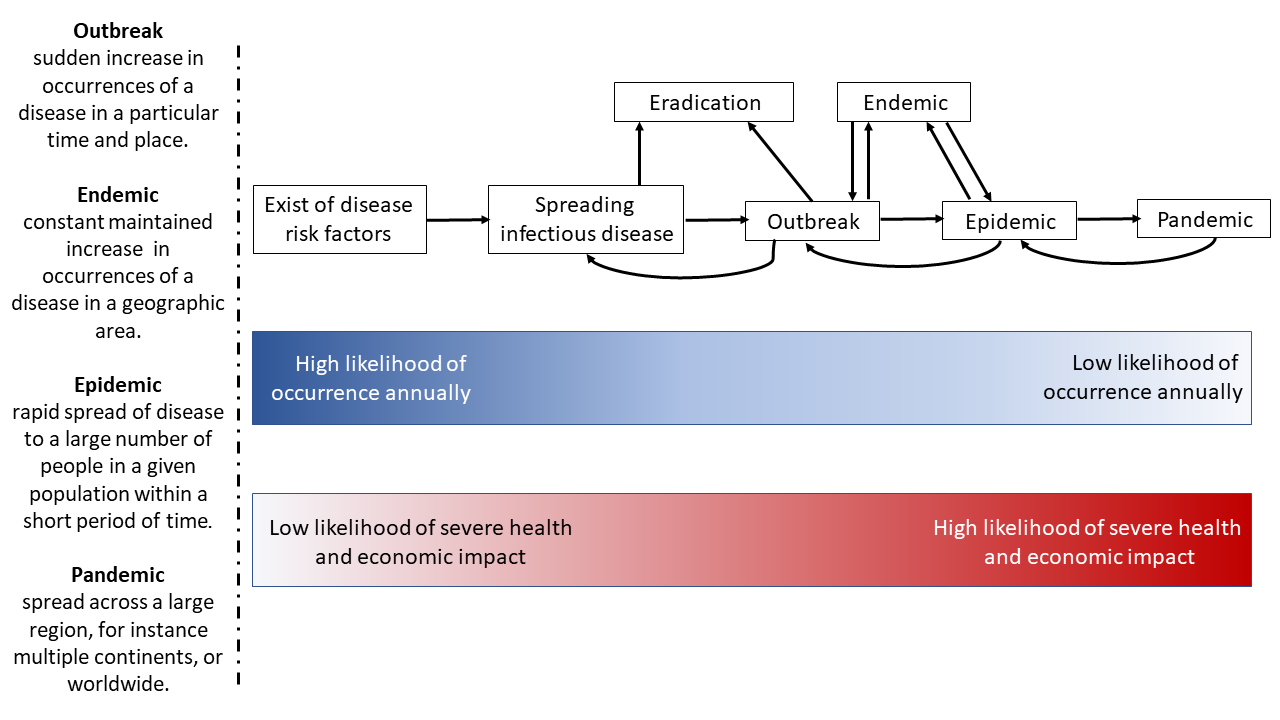
\includegraphics[width=\textwidth]{FIGS/Difference_between_outbreak,_endemic,_epidemic_and_pandemic-en.png}
\end{frame}
        

%%%%%%%%%%%%%%%%%%%%
%%%%%%%%%%%%%%%%%%%%
\subsection{Mathematical epidemiology -- The early years}
\newSubSectionSlide{FIGS-slides-admin/Gemini_Generated_Image_9agynl9agynl9agy.jpeg}

\begin{frame}{Daniel Bernoulli (1760)}
\begin{minipage}{0.47\textwidth}
\bbullet \href{https://gallica.bnf.fr/ark:/12148/bpt6k3558n/f220.item}{BNF scan} or \href{https://julien-arino.github.io/assets/pdf/Bernoulli-1760.pdf}{pdf}
\vskip1cm
\bbullet Probably the first epidemic model
\vskip1cm
\bbullet About petite vérole (smallpox) inoculation    
\end{minipage}
\begin{minipage}{0.5\textwidth}
    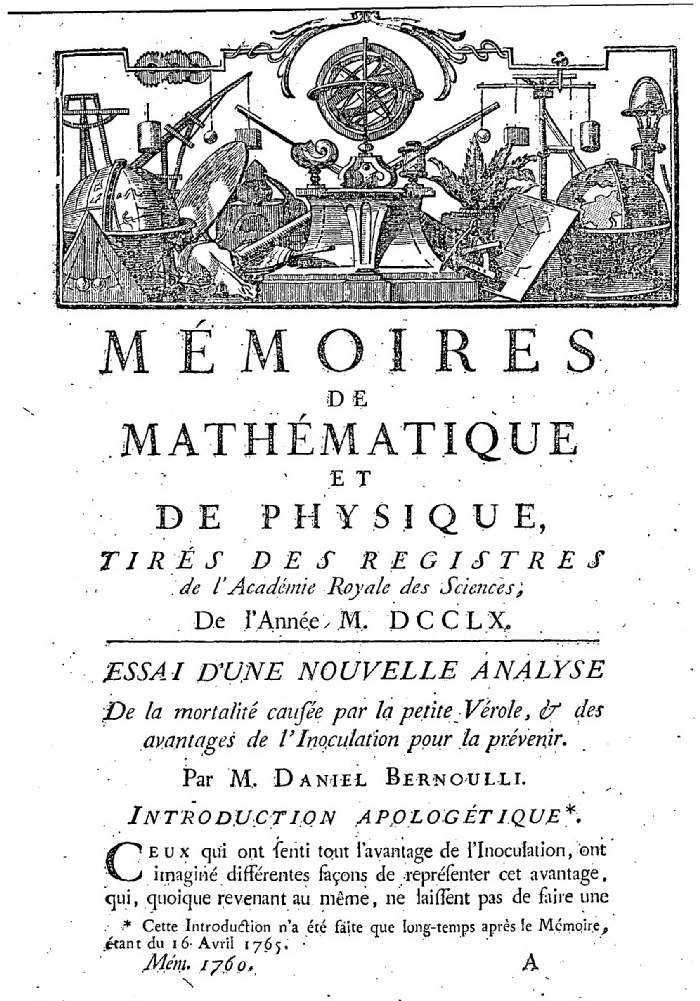
\includegraphics[width=0.8\textwidth]{FIGS/Bernoulli-1760-first_page.jpg}
\end{minipage}
\end{frame}


\begin{frame}{Ross (early 1900)}
\begin{minipage}{0.6\textwidth}
\bbullet On 20 August 1897, observed malaria parasites in the gut of a mosquito fed several days earlier on a malaria positive human
\vskip1cm
\bbullet Nobel Prize for Medicine 1902
\vskip1cm
\bbullet Started considering malaria eradication using mathematical models; for some history, read \href{https://www.ncbi.nlm.nih.gov/pmc/articles/PMC3320609/pdf/ppat.1002588.pdf}{this 2012 paper}
\end{minipage}\quad
\begin{minipage}{0.37\textwidth}
    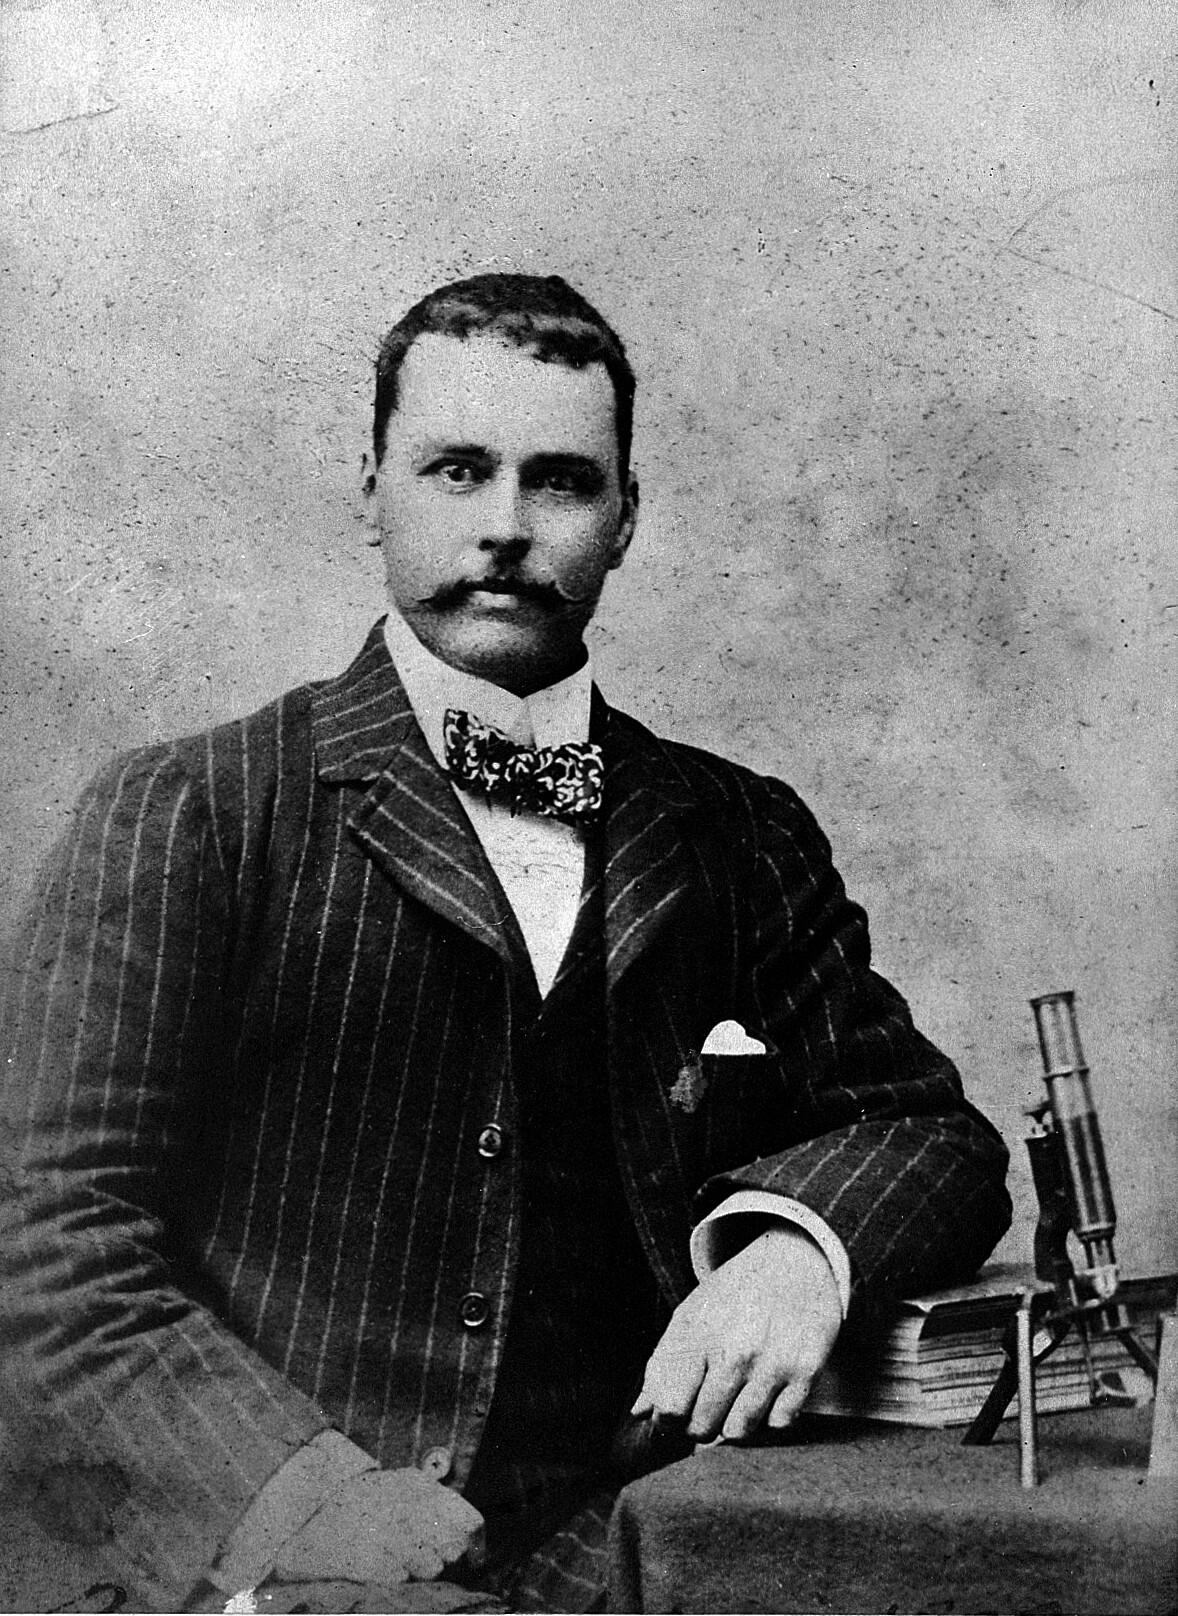
\includegraphics[width=0.8\textwidth]{FIGS/RonaldRoss_WellcomeCollection.jpg}
\end{minipage}
\end{frame}


\begin{frame}{Kermack and McKendrick (1927+)}
Model in these slides is a particular case in
\begin{itemize}
  \item Kermack \& McKendrick. \href{https://doi.org/10.1098/rspa.1927.0118}{A contribution to the mathematical theory of epidemics} (1927)
\end{itemize}
\vfill
That paper was followed by a series of ``Contributions to the mathematical theory of epidemics.''
\begin{itemize}
  \item \href{https://doi.org/10.1098/rspa.1932.0171}{II. The problem of endemicity} (1932)
  \item \href{https://doi.org/10.1098/rspa.1933.0106}{III. Further studies of the problem of endemicity} (1933)
  \item \href{https://doi.org/10.1017/S0022172400034902}{IV. Analysis of experimental epidemics of the virus disease mouse ectromelia} (1937)
  \item \href{https://doi.org/10.1017/S0022172400011918}{V. Analysis of experimental epidemics of mouse-typhoid; a bacterial disease conferring incomplete immunity} (1939)
\end{itemize}
\end{frame}


\begin{frame}{Macdonald, Dietz and malaria}
\bbullet Read for instance \href{https://doi.org/10.1371/journal.ppat.1002588}{this paper}, which presents a history of the development of the so-called Ross-Macdonald model
\vfill
\bbullet Klaus Dietz also worked a lot on malaria
\end{frame}
    
    
\begin{frame}{Some activity later, but not much until 1990s}
\bbullet In recent years, explosion
\vfill
\bbullet Since the beginning of COVID-19: just nuts..
\end{frame}

\begin{frame}{Some landmarks in mathematical epidemiology (IMBO)}
\bbullet Macdonald. The epidemiology and control of malaria. 1957
\vfill
\bbullet Baroyan, Rvachev et al. Deterministic epidemic models for a territory with a transport network. Kibernetika, 1967
\vfill
\bbullet Hethcote \& Yorke. Gonorrhea Transmission Dynamics and Control. LNBM 56, 1984
\vfill
\bbullet Anderson \& May. Infectious diseases of humans: dynamics and control. 1991
\vfill
\bbullet Capasso. Mathematical Structures of Epidemic Systems. LNBM 97, 1993
\vfill
\bbullet Hethcote. The mathematics of infectious diseases. SIAM Review, 2000
\vfill
\bbullet van den Driessche \& Watmough. Reproduction numbers and sub-threshold endemic equilibria for compartmental models of disease transmission. MBS, 2002      
\end{frame}


%%%%%%%%%%%%%%%%%%%%
%%%%%%%%%%%%%%%%%%%%
\subsection{Computational epidemiology}
\newSubSectionSlide{FIGS-slides-admin/Gemini_Generated_Image_9agynl9agynl9agy.jpeg}


\begin{frame}{A more recent trend}
\bbullet Some rare numerical work $\leq$ 1980s, mostly simulation of math models
\begin{itemize}
    \item Baroyan, Rvachev et al. \href{https://doi.org/10.2307/1426167}{Computer modelling of influenza epidemics for the whole country (USSR)}. \emph{Advances in Applied Probability} (1971) 
    \item Rvachev \& Longini. \href{https://doi.org/10.1016/0025-5564(85)90064-1}{A mathematical model for the global spread of influenza}. \emph{Mathematical Biosciences} (1986) 
    \item Flahault, Letrait et al. \href{https://doi.org/10.1002/sim.4780071107}{Modelling the 1985 influenza epidemic in France}. \emph{Statistics in Medicine} (1988)
\end{itemize}
\vfill
\bbullet More and more frequent now, to the point that some modelling studies are purely simulation-based
\end{frame}

\begin{frame}{Agent-based models (ABM)}
\bbullet Early in the life of these models, they were called IBM (individual-based models)
\vfill
\bbullet Over the years, a "philosophical" distinction has emerged:
\begin{itemize}
\item IBM are mathematical models that consider individuals as the units; e.g., DTMC, CTMC, branching processes, etc.
\item ABM are computational models whose study is, for the most part, only possible numerically
\end{itemize}
\end{frame}

\begin{frame}{Network models}
\bbullet Network models endow vertices with simple systems and couple them through graphs
\vfill
\bbullet Can be ABM, but some networks can also be studied analytically
\end{frame}

%%%%%%%%%%%%%%%%%%%%
%%%%%%%%%%%%%%%%%%%%
\subsection{Use of data in mathematical epidemiology}
\newSubSectionSlide{FIGS-slides-admin/Gemini_Generated_Image_9agynl9agynl9agy.jpeg}


\begin{frame}{Has happened all along, undergoing a transformation}
\bbullet Epidemiology has long relied on data
\vfill
\bbullet Many developments in statistics originate there
\vfill
\bbullet Data has traditionally been better for chronic diseases than for infectious ones
\vfill
\bbullet Near-real-time surveillance of infectious diseases ongoing since the 1980s (e.g., Réseau Sentinelles)
\vfill
\bbullet SARS-CoV-1 saw the beginning of a move towards real-time emerging infectious disease data
\vfill
\bbullet With SARS-CoV-2, the system has really progressed a lot, both in terms of ``citizen science'' and governmental initiatives
\end{frame}



%%%%%%%%%%%%%%%%%%%%
%%%%%%%%%%%%%%%%%%%%
\subsection{Compartmental models}
\newSubSectionSlide{FIGS-slides-admin/Gemini_Generated_Image_vqpscpvqpscpvqps.jpeg}


\begin{frame}{Compartmental models}
\bbullet Have become synonymous with epidemiological models
\vfill
\bbullet Many epidemiological models are compartmental models, but the development of compartmental models in the 1970-1980s was not at all specific to epidemiology
\vfill
\bbullet See in particular the works of \href{https://www.semanticscholar.org/author/J.-Jacquez/2321059}{John Jacquez}, \href{https://scholar.google.ca/citations?user=dv_z_mAAAAAJ}{Carl Simon}, \href{https://www.semanticscholar.org/author/G.-Walter/1799059}{GG Walter}
\vfill
\bbullet Unjustly fell into disuse: there are some very nice results in the area    
\end{frame}

\begin{frame}{Compartment (\href{https://doi-org.uml.idm.oclc.org/10.1016/B978-0-12-434180-7.50021-8}{Jacquez 1979})}

\begin{quote}
  A \defword{compartment} is an amount of some material which acts kinetically like a distinct, homogeneous, well-mixed amount of material. A \defword{compartmental system} consists of one or more compartments which interact by exchanging the material. There may be inputs into one or more compartments from outside the system and there may be excretions from the compartments of the system.   
\end{quote}
\end{frame}

\begin{frame}{}
  \begin{minipage}{0.4\textwidth}
    \tikzstyle{cloud} = [rectangle, 
    draw=yellow!90, 
    fill=yellow!30, 
    thick, 
    minimum width=0.6cm,
    minimum height = 1cm]
    \tikzstyle{line} = [draw, 
    -latex', 
    color=black]
    \begin{tikzpicture}[scale=1.5, transform shape]
      \node [cloud] (S) {$q_i$};
      \coordinate[above=of S] (h1);
      \coordinate[right=of S] (h2);
      \coordinate[left=of S] (h3);
      \coordinate[below=of S] (h4);
      %% Flows
      \path [line, very thick] (h1) to node [midway, right] (TextNode) {$i_i(t)$} (S);
      \path [line, very thick] (S) to node [midway, above] (TextNode) {$f_{ji}$} (h2);
      \path [line, very thick] (h3) to node [midway, above] (TextNode) {$f_{ij}$} (S);
      \path [line, very thick] (S) to node [midway, right] (TextNode) {$f_{0i}$} (h4);
    \end{tikzpicture}  
  \end{minipage}
  \begin{minipage}{0.55\textwidth}
    \begin{itemize}
      \item $q_i$ size of the compartment, i.e., quantity of kinetically homogeneous material present in $i$; $q_i\geq 0$ 
      \item $f_{ij}$ and $f_{ji}$ transfer coefficients/functions
      \item $f_{0i}$ excretion coefficient/function
      \item $i_i(t)$ entries from outside the system
    \end{itemize}
  \end{minipage}
  \vfill
  Above is a \defword{flow diagram}, which summarises the different flows acting on the compartment
\end{frame}


%%%%%%%%%%%%%%%%%%%%
%%%%%%%%%%%%%%%%%%%%
%%%%%%%%%%%%%%%%%%%%
%%%%%%%%%%%%%%%%%%%%
\section{Kermack-McKendrick-type epidemic models}
\newSectionSlide{FIGS-slides-admin/Gemini_Generated_Image_vqpscpvqpscpvqps.jpeg}

\maxFrameImage{FIGS/KMK-title-page}


\begin{frame}{What is the \emph{size} of an epidemic?}
\bbullet 
If we are interested in the possibility that an epidemic occurs
\begin{itemize}
  \item Does an epidemic peak always take place?
  \item If it does take place, what is its size?
\end{itemize}
\vfill
\bbullet If an epidemic traverses a population, is everyone affected/infected?
\end{frame}


%%%%%%%%%%%%%%%%%%%%
%%%%%%%%%%%%%%%%%%%%
\subsection{The Kermack-McKendrick (KMK) model}
\newSubSectionSlide{FIGS-slides-admin/Gemini_Generated_Image_vqpscpvqpscpvqps.jpeg}

\maxFrameImage{FIGS/KMK-model-in-paper}


\begin{frame}{The Kermack-McKendrick SIR model without demography}
\bbullet The period of time under consideration is sufficiently short that demography can be neglected (we also say the model has \emph{no vital dynamics})
\vfill
\bbullet Individuals are either \emph{susceptible} to the disease or \emph{infected} by (and \emph{infectious} with) the disease
\vfill
\bbullet After recovering or dying from the disease, individuals are \emph{removed} from the infectious compartment ($R$)
\vfill
\bbullet Incidence is of \defword{mass action} type and takes the form $\beta SI$
\end{frame}


\begin{frame}{The state variables}
We formulate the model as a system of \defword{differential equations}
\vfill
Differential equations: unknowns are \emph{functions} (instead of scalars, like in algebraic equations)
\vfill
At time $t\geq 0$ (we typically assume time starts at $t=0$, but could also consider $t\geq t_0>0$), the \defword{state variables}, in the current model, are the numbers of individuals who are
\begin{itemize}
\item susceptible to the disease: $S(t)$
\item infected and infectious with the disease: $I(t)$
\item removed from the infectious comparment: $R(t)$
\end{itemize}
\vfill
Often, we drop the dependence on $t$ if it is not explicitly required and write $S,I,R$
\end{frame}



\begin{frame}{Important -- Incidence functions}
Incidence is the rate at which new cases arise, the incidence function then describes how contacts lead to new infections
\vfill
If there are $S$ susceptible individuals and $I$ infectious individuals in the population, we use a function of the form
\[
f(S,I)
\]
The function can also explicitly depend on the total population $N$, i.e., $f(S,I,N)$
\vfill
We return to incidence functions in \href{no.se}{Lecture 06}
\vfill
For now, just know the most common incidence functions are
\begin{itemize}
\item \defword{mass action incidence} $f(S,I,N)=\beta SI$
\item \defword{standard} (or \defword{proportional}) \defword{incidence} $f(S,I,N)=\beta SI/N$
\end{itemize}
\end{frame}



\begin{frame}{The Kermack-McKendrick model}
This model is typically called the \defword{Kermack-McKendrick} (KMK) \defword{SIR model} 
  \begin{align*}
    \frac{d}{dt}S(t) &= -\beta S(t)I(t) \\
    \frac{d}{dt}I(t) &= \beta S(t)I(t)-\gamma I(t) \\
    \frac{d}{dt}R(t) &= \gamma I(t) 
    \end{align*}  
\vfill
\begin{center}
  \begin{tikzpicture}[scale=1.25, transform shape]
    \node [circle, fill=green!50, text=black] (S) {$S(t)$};
    \node [circle, right=1.5cm of S, fill=red!90, text=black] (I) {$I(t)$};
    \node [circle, right=1.5cm of I, fill=blue!90, text=black] (R) {$R(t)$};
    %% Flows
    \path [line, very thick] (S) to node [midway, above] (TextNode) {$\beta S(t)I(t)$} (I);
    \path [line, very thick] (I) to node [midway, above] (TextNode) {$\gamma I(t)$} (R);
  \end{tikzpicture}    
\end{center}
\end{frame}



\begin{frame}{The Kermack-McKendrick model}
As indicated, we often drop dependence on $t$ of the state variables; we also write $X':=dX(t)/dt$. So the KMK model is usually written
\vfill
\begin{subequations}\label{sys:KMK}
  \begin{align}
    S\pprime &= -\beta SI \label{sys:KMK_dS} \\
    I\pprime &= \beta SI-\gamma I \label{sys:KMK_dI} \\
    R\pprime &= \gamma I \label{sys:KMK_dR}
    \end{align}  
\end{subequations}
\vfill
\begin{center}
  \begin{tikzpicture}[scale=1.5, transform shape]
    \node [circle, fill=green!50, text=black] (S) {$S$};
    \node [circle, right=1cm of S, fill=red!90, text=black] (I) {$I$};
    \node [circle, right=1cm of I, fill=blue!90, text=black] (R) {$R$};
    %% Flows
    \path [line, very thick] (S) to node [midway, above] (TextNode) {$\beta SI$} (I);
    \path [line, very thick] (I) to node [midway, above] (TextNode) {$\gamma I$} (R);
  \end{tikzpicture}    
\end{center}
\end{frame}

%%%%%%%%%%%%%%%%%%%%
%%%%%%%%%%%%%%%%%%%%
\subsection{Mathematical analysis of KMK}
\newSubSectionSlide{FIGS-slides-admin/Gemini_Generated_Image_vqpscpvqpscpvqps.jpeg}


\begin{frame}{Reduction of the model}
  3 compartments, but when considered in detail, we notice that \emph{removed} do not have a direct influence on the dynamics of $S$ or $I$, in the sense that $R$ does not appear in \eqref{sys:KMK_dS} or \eqref{sys:KMK_dI}
  \vfill
  Furthermore, the total population (including deceased who are also in $R$) $N=S+I+R$ satisfies
  \[
  N\pprime=(S+I+R)'=0
  \]
  Thus, $N$ is constant and 
  \begin{equation}\label{eq:constant_population}
    S(t)+I(t)+R(t)=N_0,\quad t\geq 0.
  \end{equation}
  so the dynamics of $R$ can be deduced from $R=N-(S+I)$.
  So we can consider
  \begin{subequations}\label{sys:KMK_2d}
    \begin{align}
      S\pprime &= -\beta SI \label{sys:KMK_2d_dS}\\
      I\pprime &= \beta SI-\gamma I  \label{sys:KMK_2d_dI}
      \end{align}
    \end{subequations}
\end{frame}

\begin{frame}{Equilibria}
  Let us consider the equilibria of
  \begin{subequations}
    \begin{align}
      S\pprime &= -\beta SI 
      \tag{\ref{sys:KMK_2d_dS}} \\
      I\pprime &= (\beta S-\gamma)I  
      \tag{\ref{sys:KMK_2d_dI}}
    \end{align}
  \end{subequations}
\vfill
  From \eqref{sys:KMK_2d_dI}
  \begin{itemize}
    \item either $S^\star=\gamma/\beta$ 
    \item or $I^\star=0$
  \end{itemize}
  \vfill
  Substitute into \eqref{sys:KMK_2d_dS}
  \begin{itemize}
    \item in the first case, $(S^\star,I^\star)=(\gamma/\beta,0)$ 
    \item in the second case, any $S^\star\geq 0$ is an EP
  \end{itemize}
  \vfill
  The second case is an \emph{issue}: the usual linearisation does not work when there is a \emph{continuum} of equilibria as the EP are not \emph{isolated}
\end{frame}

\begin{frame}{What is the problem with non-isolated EP?}
\begin{proposition}\label{prop:EP_KMK}
The Kermack-McKendrick model SIR model \eqref{sys:KMK} has the continuum of equilibria
\begin{equation}
\label{eq:DFE_KMK}
    E_0^\text{KMK}:=\left\{
    (S^\star,I^\star,R^\star)=(S_\infty,0,N_0-S_\infty),\quad S_\infty\in[0,N_0]
    \right\}
\end{equation}
\end{proposition}
\end{frame}

\begin{frame}{Proof}
Let us consider \eqref{sys:KMK} and start with $I=I^\star=0$.
Substitute this value into \eqref{sys:KMK_dS} at equilibrium, giving $0 = -\gamma S^\star I^\star(=0)$, meaning that any value of $S^\star$ satisfies this relation. From the conservation of the total population \eqref{eq:constant_population}, the equilibrium $E_0^\text{KMK}$ takes the form given by \eqref{eq:DFE_KMK}
\vfill
Now consider $S=S^\star=\gamma/\beta$. Substituting this value into \eqref{sys:KMK_dS} at equilibrium gives $0 = -\gamma I^\star$, from which it follows that $I^\star=0$, and, using the conservation of total population \eqref{eq:constant_population},
\begin{equation}\label{eq:DFE_KMK_tmp}
    (S^\star,I^\star,R^\star)=\left(
    \frac{\gamma}{\beta},0,N_0-\frac{\gamma}{\beta}
    \right)
\end{equation}
is an equilibrium of \eqref{sys:KMK}. 
The equilibrium \eqref{eq:DFE_KMK_tmp} is biologically relevant only when $N_0-\gamma/\beta\geq 0$.
Note that \eqref{eq:DFE_KMK} includes \eqref{eq:DFE_KMK_tmp} when the latter is biologically relevant
\end{frame}

\begin{frame}
Adapting slightly the definitions in \cite{HirschSmale1974}, consider the ordinary differential equation
\begin{equation}\label{eq:ODE}
    x' = f(x)
\end{equation}
where $x(t)\in W$ and $f:W\to E$ is a function such that solutions to \eqref{eq:ODE} exist uniquely, e.g., a $C^1$ function, from an open set $W$ of the vector space $E$ into $E$
\vfill
Denote $x(t,x_0)$ the solution to \eqref{eq:ODE} through the initial value $x(t_0)=x_0$
\end{frame}

\begin{frame}
A point $x^\star\in W$ is an \defword{equilibrium} if $f(x^\star)=0$
\vfill
\begin{definition}[Locally stable equilibrium]\label{def:LS_EP}
An equilibrium point $x^\star$ of \eqref{eq:ODE} is \defword{locally stable} (LS) if for every neighbourhood $\mathcal{N}(x^\star)$ of $x^\star$ in $W$, there is a neighbourhood $\mathcal{N}_1\subseteq\mathcal{N}(x^\star)$ of $x^\star$ such that every solution $x(t,x_0)$ with $x_0\in\mathcal{N}_1$ is defined and in $\mathcal{N}(x^\star)$ for all $t>t_0$
\end{definition}
\vfill
\begin{definition}[Locally asymptotically stable equilibrium]
If $\mathcal{N}_1$ can be chosen so that in addition to the properties in Definition~\ref{def:LS_EP}, $\lim_{t\to\infty}x(t,x_0)=x^\star$ for all $x_0\in\mathcal{N}_1$, then $x^\star$ is \defword{locally asymptotically stable} (LAS)
\end{definition}
\end{frame}

\begin{frame}
DFE \eqref{eq:DFE_KMK} of \eqref{sys:KMK} are not \defword{isolated}: any (open) neighbourhood of an equilibrium contains infinitely many other equilibria
\vfill
    \begin{tikzpicture}
    \coordinate (SN) at (4,0);
    \coordinate (RN) at (0,4);
    \coordinate (xs) at (1.5,2.5);
    % The region
    \fill[gray!10] (0,4) -| (4,4) -| (4,0) -| (0,0) -- cycle;
    \draw[gray!40, thick]  (0,0) -- (4,0) -- (4,4) -- (0,4) -- cycle;
    % axis, on the top
    \draw[->] (0,0) -- (5.25,0) node[below left] {$S$};
    \draw[->] (0,0) -- (0,5) node[below left] {$R$};
    % The line of EP
    \draw[thin] (SN) -- (RN) node[pos=0.3,right] {$S+R=N_0$};
    \draw[line width=2] (1,3) -- (2,2);
    \shade[ball color = gray!40, opacity = 0.4] (xs) circle (0.72);
    % Intersections on S and R axes
    \draw (SN) circle (0.1cm) node[below] {$S=N_0$};
    \shade[ball color = blue, opacity = 1] (SN) circle (0.1cm);
    \draw (RN) circle (0.1cm) node[left] {$R=N_0$};
    \shade[ball color = blue, opacity = 1] (RN) circle (0.1cm);
    % The equilibrium
    \draw (xs) circle (0.1cm) node[above right] {$x^\star$};
    \shade[ball color = red, opacity = 1] (xs) circle (0.1cm);
    \end{tikzpicture} 
    \vfill
Neighbourhood $\N(x^\star)$ of $x^\star\in E_0^\text{KMK}$ lying on the $S-R$ plane (the neighbourhood extends above and below the $S-R$ plane in the $I$ direction, not shown here). 
The thin line is $E_0^\text{KMK}$, the thick line is $E_0^\text{KMK}\cap\N(x^\star)$
\end{frame}

\begin{frame}
\begin{proposition}
Consider a disease-free equilibrium $x^\star\in E_0^\text{KMK}$ of \eqref{sys:KMK}. Then $x^\star$ is LS but not LAS  
\end{proposition}
\vfill
This means in particular that considering the Jacobian of \eqref{sys:KMK} at the DFE \textbf{makes no sense}!
\end{frame}

\begin{frame}{Proof}
Let $x_1^\star\in E_0^\text{KMK}$ be an equilibrium of \eqref{sys:KMK}.
Consider $\S_\mathcal{N}(x_1^\star)\subset E_0^\text{KMK}$, open subset of $E_0^\text{KMK}$ containing $x_1^\star$.
Now take some $x_2^\star\in\S_\mathcal{N}(x_1^\star)$. Since $x_2^\star\in\S_\mathcal{N}(x_1^\star)\subset E_0^\text{KMK}$, $x_2^\star$ is an equilibrium of \eqref{sys:KMK} and thus $x(t,x_2^\star)=x_2^\star\in\S_\mathcal{N}(x_1^\star)$ for all $t\geq t_0$.
As a consequence, $x_1^\star$ is locally stable
\vfill
$\Rightarrow$ any open neighbourhood $\mathcal{N}(x_1^\star)$ contains $\S_\mathcal{N}=\mathcal{N}(x_1^\star)\cap E_0^\text{KMK}$
\vfill
Consider, then, some $x_2^\star\in\S_\mathcal{N}$.
Since $x_2^\star\in\S_\mathcal{N}$, $x_2^\star$ is an equilibrium and as a consequence, $\lim_{t\to\infty}x(t,x_2^\star)=x_2^\star$.
Therefore, any open neighbourhood of $x_1^\star$ contains points $x_0$ not such that $\lim_{t\to\infty}x(t,x_0)=x_1^\star$ $\implies$ $x_1^\star$ is LS but not LAS
\end{frame}

\begin{frame}{The next generation matrix method in this context}
Consider the method in \cite{VdDWatmough2002}
\vfill
To construct $\R_0$, they require \emph{local stability}
\vfill
Theorem 2 in \cite{VdDWatmough2002} pertaining to LAS, on the other hand, has one assumption (assumption A5) that the DFE be \emph{locally asymptotically stable}, with the assumption that all eigenvalues of the linearisation near a disease-free equilibrium have negative real parts
\vfill
Clearly, this cannot be true with \eqref{sys:KMK}
\end{frame}


\begin{frame}{Another approach -- Study $dI/dS$}
  \begin{align}
  S\pprime &= -\beta SI \tag{\ref{sys:KMK_2d_dS}}\\
  I\pprime &= \beta SI-\gamma I  \tag{\ref{sys:KMK_2d_dI}}
  \end{align}
  \vfill
  What is the dynamics of $dI/dS$? 
  \begin{equation}
    \label{eq:KMK_dI_over_dS}
    \frac{dI}{dS}
    =\frac{dI}{dt}\frac{dt}{dS}
    =\frac{I'}{S'}
    =\frac{\beta SI-\gamma I}{-\beta SI}
    =\frac{\gamma}{\beta S}-1
  \end{equation}
 provided $S\neq 0$
  \vfill
  \textbf{Note --} Recall that $S$ and $I$ are $S(t)$ and $I(t)$.. \eqref{eq:KMK_dI_over_dS} thus describes the relation between $S$ and $I$ over solutions to the original ODE \eqref{sys:KMK_2d}
\end{frame}


\begin{frame}{}
  Integrate $\eqref{eq:KMK_dI_over_dS}$ and obtain trajectories in state space
  $$
  I(S)=\frac\gamma\beta \ln S-S+C
  $$
  with $C\in\IR$
  \vfill
  IC $I(S_0)=I_0$ $\Rightarrow$ $C=S_0+I_0-\dfrac \gamma\beta \ln S_0$ and the solution to \eqref{sys:KMK} is, as a function of $S$
  \begin{align*}
  I(S)&=S_0+I_0-S+\frac\gamma\beta \ln \frac S{S_0} \\
  R(S)&=N-S-I(S)=R_0-\frac\gamma\beta \ln \frac S{S_0}
  \end{align*}
  (since $N_0=S_0+I_0+R_0$)
\end{frame}




\begin{frame}
Trajectories of \eqref{sys:KMK_2d} in $(S,I)$-space, normalised, with IC $(S_0,1-S_0)$ and $\beta/\gamma=2.5$
\vfill
\begin{center}
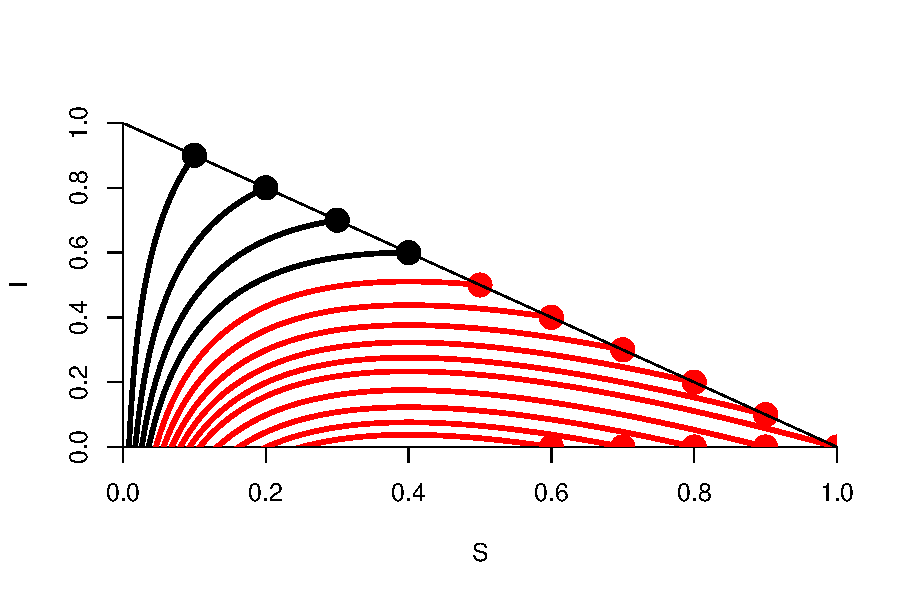
\includegraphics[width=0.9\textwidth]{FIGS/course-01-KMK_SI_plane-1.pdf}
\end{center}
\end{frame}



\begin{frame}{}
  Let us study
  $$
  I(S)=S_0+I_0-S+\frac\gamma\beta \ln \frac S{S_0} 
  $$
  We have
  $$
  \frac{d}{dS}I(S) = \frac{\gamma}{\beta S}-1
  $$
  So, in the previous curves, the max of $I(S)$ happens when $S=\gamma/\beta$ ($S=0.4$ in the example)
  \vfill
  At that point,
  $$
  I(S) = I_0+\left(
    1-\frac{1}{\R_0} - \frac{\ln(\R_0)}{\R_0}
  \right)S_0
  $$
\end{frame}


\begin{frame}{}
  \begin{theorem}[Epidemic or no epidemic?]
    Let $(S(t),I(t))$ be a solution to \eqref{sys:KMK_2d} and $\R_0$ defined by
    \begin{equation}\label{eq:R0_KMK}
    \R_0=\frac{\beta}{\gamma}S_0
    \end{equation}
    \vfill
    \begin{itemize}
      \item If $\R_0\leq 1$, then $I(t)\searrow 0$ when $t\to\infty$ 
      \item If $\R_0>1$, then $I(t)$ first reaches a maximum 
      \begin{equation}\label{eq:max_I}
        I_0+\left(
      1-\frac{1}{\R_0} - \frac{\ln(\R_0)}{\R_0}
      \right)S_0
      \end{equation}
      then goes to 0 as $t\to\infty$  
    \end{itemize}    
  \end{theorem}
\end{frame}

\begin{knitrout}
\definecolor{shadecolor}{rgb}{0.969, 0.969, 0.969}\color{fgcolor}\begin{kframe}
\begin{alltt}
\hldef{rhs_SIR_KMK} \hlkwb{<-} \hlkwa{function}\hldef{(}\hlkwc{t}\hldef{,} \hlkwc{x}\hldef{,} \hlkwc{p}\hldef{) \{}
  \hlkwd{with}\hldef{(}\hlkwd{as.list}\hldef{(}\hlkwd{c}\hldef{(x, p)), \{}
    \hldef{dS} \hlkwb{=} \hlopt{-} \hldef{beta} \hlopt{*} \hldef{S} \hlopt{*} \hldef{I}
    \hldef{dI} \hlkwb{=} \hldef{beta} \hlopt{*} \hldef{S} \hlopt{*} \hldef{I} \hlopt{-} \hldef{gamma} \hlopt{*} \hldef{I}
    \hldef{dR} \hlkwb{=} \hldef{gamma} \hlopt{*} \hldef{I}
    \hlkwd{return}\hldef{(}\hlkwd{list}\hldef{(}\hlkwd{c}\hldef{(dS, dI, dR)))}
  \hldef{\})}
\hldef{\}}
\hlcom{# Initial condition for S (to compute R_0)}
\hldef{S0} \hlkwb{=} \hlnum{1000}
\hldef{gamma} \hlkwb{=} \hlnum{1}\hlopt{/}\hlnum{14}
\hlcom{# Set beta so that R_0 = 1.5}
\hldef{beta} \hlkwb{=} \hlnum{1.5} \hlopt{*} \hldef{gamma} \hlopt{/} \hldef{S0}
\hldef{params} \hlkwb{=} \hlkwd{list}\hldef{(}\hlkwc{gamma} \hldef{= gamma,} \hlkwc{beta} \hldef{= beta)}
\hldef{IC} \hlkwb{=} \hlkwd{c}\hldef{(}\hlkwc{S} \hldef{= S0,} \hlkwc{I} \hldef{=} \hlnum{1}\hldef{,} \hlkwc{R} \hldef{=} \hlnum{0}\hldef{)}
\hldef{times} \hlkwb{=} \hlkwd{seq}\hldef{(}\hlnum{0}\hldef{,} \hlnum{365}\hldef{,} \hlnum{1}\hldef{)}
\hldef{sol_KMK} \hlkwb{<-} \hlkwd{ode}\hldef{(IC, times, rhs_SIR_KMK, params)}
\end{alltt}
\end{kframe}
\end{knitrout}



\begin{frame}[fragile]{}
\begin{knitrout}
\definecolor{shadecolor}{rgb}{0.969, 0.969, 0.969}\color{fgcolor}\begin{kframe}
\begin{alltt}
\hlkwd{plot}\hldef{(sol_KMK[,} \hlsng{"time"}\hldef{], sol_KMK[,} \hlsng{"I"}\hldef{],}
     \hlkwc{type} \hldef{=} \hlsng{"l"}\hldef{,} \hlkwc{lwd} \hldef{=} \hlnum{2}\hldef{,}
     \hlkwc{main} \hldef{=} \hlkwd{TeX}\hldef{(}\hlsng{"Kermack-McKendrick SIR, $R_0=1.5$"}\hldef{),}
     \hlkwc{xlab} \hldef{=} \hlsng{"Time (days)"}\hldef{,} \hlkwc{ylab} \hldef{=} \hlsng{"Prevalence"}\hldef{)}
\end{alltt}
\end{kframe}
\end{knitrout}
\begin{center}
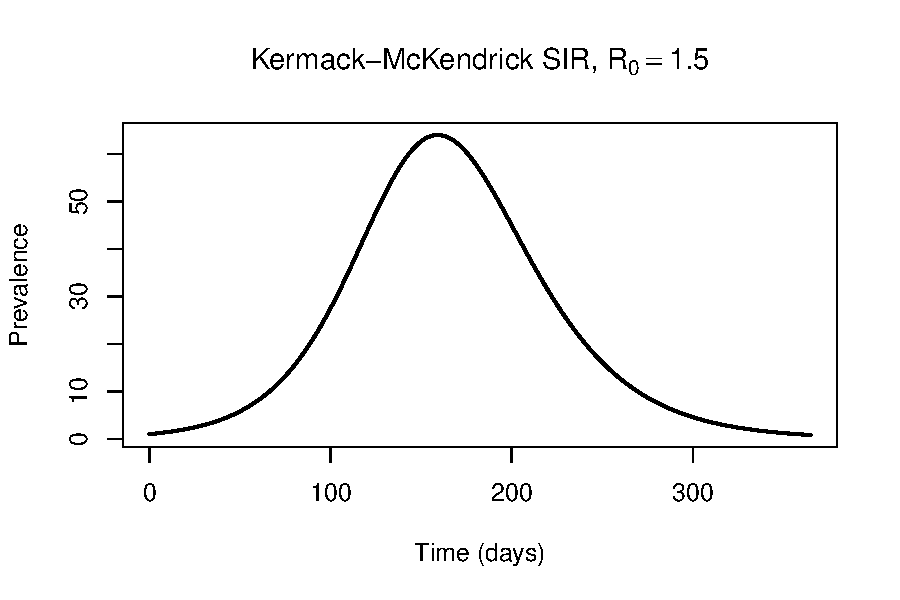
\includegraphics[width=0.8\textwidth]{FIGS/course-01-KMK_R0eq1dot5-1.pdf}
\end{center}
\end{frame}


\begin{frame}{The basic reproduction number $\R_0$}
\bbullet Indicator often used in epidemiology. Verbally
\begin{quote}
  average number of secondary cases of infection produced when a single infectious individual is introduced in a wholly susceptible population
\end{quote}
\vfill
\bbullet If $\R_0<1$, then each infectious individual infects on average less than 1 person and the epidemic is quite likely to go extinct 
\vfill
\bbullet If $R_0>1$, then each infectious individual infects on average more than 1 person and an epidemic is quite likely to occur
\end{frame}

\begin{frame}{A few sample values of $\R_0$}
  $\R_0$ can be estimated from data (from the Anderson \& May book)
  \vfill
  \begin{center}
  \begin{tabular}{llcc}
  \hline 
  Infection & Location & Period & $\R_0$ \\
  \hline
  Measles & Cirencester, England & 1947-50 & 13-14 \\
  & England and Wales & 1950-68 & 16-18 \\
  & Kansas, USA & 1918-21 & 5-6 \\
  & Ontario, Canada & 1912-3 & 11-12 \\
  & Willesden, England & 1912-3 & 11-12 \\
  & Ghana & 1960-8 & 14-15 \\
  & East Nigeria & 1960-8 & 16-17 \\
  \end{tabular}
  \end{center}
\end{frame}
    

%%%%%%%%%%%%%%%%%%%%%%%%
%%%%%%%%%%%%%%%%%%%%%%%%
\subsection{The final size of a KMK epidemic}
\newSubSectionSlide{FIGS-slides-admin/Gemini_Generated_Image_vqpscpvqpscpvqps.jpeg}

\begin{frame}{Final size of an epidemic}
  For a nonnegative valued integrable function $w(t)$, denote
  $$
  w_0=w(0),\qquad  w_\infty = \lim_{t\to\infty}w(t),\qquad\hat w = \int_0^\infty w(t)\ dt
  $$
  \vfill
  In the subsystem
  \begin{align}
  S' &= -\beta SI \tag{\ref{sys:KMK_2d_dS}} \\
  I' &= \beta SI-\gamma I \tag{\ref{sys:KMK_2d_dI}} 
  \end{align}
  compute the sum of \eqref{sys:KMK_2d_dS} and \eqref{sys:KMK_2d_dI}, making sure to show time dependence $$
  \frac{d}{dt}(S(t)+I(t))=-\gamma I(t)
  $$
\end{frame}


\begin{frame}{}
  Integrate from 0 to $\infty$:
  $$
  \int_0^\infty\frac{d}{dt}(S(t)+I(t))\ dt=-\int_0^\infty\gamma I(t)dt 
  $$
  The left hand side gives
  $$
  \int_0^\infty\frac{d}{dt}(S(t)+I(t))\ dt
  = S_\infty+I_\infty-S_0-I_0 = S_\infty-S_0-I_0
  $$
  since $I_\infty=0$
  \vfill
  The right hand side takes the form
  $$
  -\int_0^\infty\gamma I(t)dt = -\gamma\int_0^\infty I(t)dt = -\gamma \hat I
  $$
  We thus have
  \begin{equation}
  \label{eq:KMK_final_size_step1}
  S_\infty-S_0-I_0 = -\gamma\hat I
  \end{equation}
\end{frame}



\begin{frame}{}
  Now consider \eqref{sys:KMK_2d_dS}:
  $$
  S' = -\beta SI
  $$
  Divide both sides by $S$:
  $$
  \frac{S'(t)}{S(t)} = -\beta I(t)
  $$
  Integrate from 0 to $\infty$:
  \begin{equation}
  \label{eq:KMK_final_size_step2}
  \ln S_\infty-\ln S_0 = -\beta \hat I
  \end{equation}
  Express \eqref{eq:KMK_final_size_step1} and \eqref{eq:KMK_final_size_step2} in terms of $-\hat I$ and equate
  $$
  \frac{\ln S_\infty-\ln S_0}{\beta}
  =
  \frac{S_\infty-S_0-I_0}{\gamma}
  $$
  Thus we have
  \begin{equation}
  \label{eq:final_size}
  (\ln S_0-\ln S_\infty)S_0 = (S_0-S_\infty)\R_0+I_0\R_0
  \end{equation}
\end{frame}



\begin{frame}{}
\begin{theorem}[Final size relation]
  Let $(S(t),I(t))$ be a solution to \eqref{sys:KMK_2d} and $\R_0$ defined by \eqref{eq:R0_KMK}
  \vskip0.5cm
  The number $S(t)$ of susceptible individuals is a nonincreasing function and its limit $S_\infty$ is the only solution in $(0,S_0)$ of the transcendental equation
  \begin{equation}\tag{\ref{eq:final_size}}
  (\ln S_0-\ln S_\infty)S_0 = (S_0-S_\infty)\R_0+I_0\R_0
  \end{equation}
\end{theorem}
\end{frame}



\begin{frame}{The (transcendantal) final size equation}
  Rewrite the final size equation
  \begin{equation}
    \tag{\ref{eq:final_size}}
  (\ln S_0-\ln S_\infty)S_0 = (S_0-S_\infty)\R_0+I_0\R_0
  \end{equation}
  as
  \begin{equation}
  \label{eq:final_size_2}
  T(S_\infty) =(\ln S_0-\ln S_\infty)S_0
  - (S_0-S_\infty)\R_0 -I_0\R_0
\end{equation}
\vfill
Thus, we seek the zeros of the function $T(S_\infty)$
\end{frame}



\begin{frame}{}
  We seek $S_\infty$ in $(0,S_0]$ s.t. $T(S_\infty)=0$, with
  \begin{equation}\tag{\ref{eq:final_size_2}}
    T(S_\infty) =(\ln S_0-\ln S_\infty)S_0
    - (S_0-S_\infty)\R_0 -I_0\R_0      
  \end{equation}
  \vfill
  Note to begin that 
  $$
  \lim_{S_\infty\to 0}T(S_\infty)=\lim_{S_\infty\to 0}-S_0\ln(S_\infty)=\infty
  $$
  \vfill
  Differentiating $T$ with respect to $S_\infty$, we get 
  $$
  T'(S_\infty)=\R_0-S_0/S_\infty
  $$ 
  \vfill
  When $S_\infty\to 0$, $\R_0-S_0/S_\infty<0$, so $T$ decreases to $S_\infty=S_0/\R_0$
  \vfill
  So if $\R_0\leq 1$, the function $T$ is decreasing on $(0,S_0)$, while it has a minimum if $\R_0>1$
\end{frame}



\begin{frame}{Case $\R_0\leq 1$}
  \begin{equation}\tag{\ref{eq:final_size_2}}
    T(S_\infty) =(\ln S_0-\ln S_\infty)S_0
    - (S_0-S_\infty)\R_0 -I_0\R_0      
  \end{equation}
  \vfill
  \bbullet We have seen that $T$ decreases on $(0,S_0]$
  \vfill
  \bbullet Also, $T(S_0)=-I_0\R_0<0$ ($I_0=0$ is trivial and not considered)
  \vfill
  \bbullet $T$ is continuous
  \vfill
  $\implies$ there exists a unique $S_\infty\in (0,S_0]$ s.t. $T(S_\infty)=0$
\end{frame}


\begin{frame}{Case $\R_0> 1$}
  \begin{equation}\tag{\ref{eq:final_size_2}}
    T(S_\infty) =(\ln S_0-\ln S_\infty)S_0
    - (S_0-S_\infty)\R_0 -I_0\R_0      
  \end{equation}
  \vfill
  \bbullet We have seen that $T$ decreases on $(0,S_0/\R_0]$
  \vfill
  \bbullet For $S_\infty\in[S_0/\R_0]$, $T'>0$
  \vfill
  \bbullet As before, $T(S_\infty)=-I_0\R_0$
  \vfill
  \bbullet $T$ is continuous
  \vfill
  $\implies$ there exists a unique $S_\infty\in (0,S_0]$ s.t. $T(S_\infty)=0$. More precisely, in this case, $S_\infty\in(0,S_0/\R_0)$
\end{frame}



\begin{frame}[fragile]{}
We solve numerically. We need a function
\begin{knitrout}
\definecolor{shadecolor}{rgb}{0.969, 0.969, 0.969}\color{fgcolor}\begin{kframe}
\begin{alltt}
\hldef{final_size_eq} \hlkwb{=} \hlkwa{function}\hldef{(}\hlkwc{S_inf}\hldef{,} \hlkwc{S0} \hldef{=} \hlnum{999}\hldef{,} \hlkwc{I0} \hldef{=} \hlnum{1}\hldef{,} \hlkwc{R_0} \hldef{=} \hlnum{2.5}\hldef{) \{}
  \hldef{OUT} \hlkwb{=} \hldef{S0}\hlopt{*}\hldef{(}\hlkwd{log}\hldef{(S0)}\hlopt{-}\hlkwd{log}\hldef{(S_inf))} \hlopt{-} \hldef{(S0}\hlopt{+}\hldef{I0}\hlopt{-}\hldef{S_inf)}\hlopt{*}\hldef{R_0}
  \hlkwd{return}\hldef{(OUT)}
\hldef{\}}
\end{alltt}
\end{kframe}
\end{knitrout}
and solve easily using \code{uniroot}:
\begin{knitrout}
\definecolor{shadecolor}{rgb}{0.969, 0.969, 0.969}\color{fgcolor}\begin{kframe}
\begin{alltt}
\hlkwd{uniroot}\hldef{(}\hlkwc{f} \hldef{= final_size_eq,} \hlkwc{interval} \hldef{=} \hlkwd{c}\hldef{(}\hlnum{0.05}\hldef{,} \hlnum{999}\hldef{))}
\end{alltt}
\begin{verbatim}
## $root
## [1] 106.8819
## 
## $f.root
## [1] -2.649285e-07
## 
## $iter
## [1] 10
## 
## $init.it
## [1] NA
## 
## $estim.prec
## [1] 6.103516e-05
\end{verbatim}
\end{kframe}
\end{knitrout}
\end{frame}


\begin{frame}[fragile]{A function to use this..}
\begin{knitrout}
\definecolor{shadecolor}{rgb}{0.969, 0.969, 0.969}\color{fgcolor}\begin{kframe}
\begin{alltt}
\hldef{final_size} \hlkwb{=} \hlkwa{function}\hldef{(}\hlkwc{L}\hldef{) \{}
  \hlkwd{with}\hldef{(}\hlkwd{as.list}\hldef{(L), \{}
  \hldef{S_inf} \hlkwb{=} \hlkwd{uniroot}\hldef{(}\hlkwc{f} \hldef{=} \hlkwa{function}\hldef{(}\hlkwc{x}\hldef{)}
    \hlkwd{final_size_eq}\hldef{(}\hlkwc{S_inf} \hldef{= x,}
                  \hlkwc{S0} \hldef{= S0,} \hlkwc{I0} \hldef{= I0,}
                  \hlkwc{R_0} \hldef{= R_0),}
    \hlkwc{interval} \hldef{=} \hlkwd{c}\hldef{(}\hlnum{0.05}\hldef{, S0))}
  \hlkwd{return}\hldef{(S_inf}\hlopt{$}\hldef{root)}
  \hldef{\})}
\hldef{\}}
\end{alltt}
\end{kframe}
\end{knitrout}
\end{frame}

\begin{frame}[fragile]{A figure with all the information}
\begin{knitrout}
\definecolor{shadecolor}{rgb}{0.969, 0.969, 0.969}\color{fgcolor}\begin{kframe}
\begin{alltt}
\hldef{N0} \hlkwb{=} \hlnum{1000}
\hldef{I0} \hlkwb{=} \hlnum{1}
\hldef{S0} \hlkwb{=} \hldef{N0}\hlopt{-}\hldef{I0}
\hldef{R_0} \hlkwb{=} \hlnum{0.8}
\hldef{S} \hlkwb{=} \hlkwd{seq}\hldef{(}\hlnum{0.1}\hldef{, S0,} \hlkwc{by} \hldef{=} \hlnum{0.1}\hldef{)}
\hldef{fs} \hlkwb{=} \hlkwd{final_size_eq}\hldef{(S,} \hlkwc{S0} \hldef{= S0,} \hlkwc{I0} \hldef{= I0,} \hlkwc{R_0} \hldef{= R_0)}
\hldef{S_inf} \hlkwb{=} \hlkwd{uniroot}\hldef{(}\hlkwc{f} \hldef{=} \hlkwa{function}\hldef{(}\hlkwc{x}\hldef{)} \hlkwd{final_size_eq}\hldef{(}\hlkwc{S_inf} \hldef{= x,}
                                              \hlkwc{S0} \hldef{= S0,} \hlkwc{I0} \hldef{= I0,}
                                              \hlkwc{R_0} \hldef{= R_0),}
                \hlkwc{interval} \hldef{=} \hlkwd{c}\hldef{(}\hlnum{0.05}\hldef{, S0))}
\hlkwd{plot}\hldef{(S, fs,} \hlkwc{type} \hldef{=} \hlsng{"l"}\hldef{,} \hlkwc{ylab} \hldef{=} \hlsng{"Value of equation (10)"}\hldef{)}
\hlkwd{abline}\hldef{(}\hlkwc{h} \hldef{=} \hlnum{0}\hldef{)}
\hlkwd{points}\hldef{(}\hlkwc{x} \hldef{= S_inf}\hlopt{$}\hldef{root,} \hlkwc{y} \hldef{=} \hlnum{0}\hldef{,} \hlkwc{pch} \hldef{=} \hlnum{19}\hldef{)}
\hlkwd{text}\hldef{(}\hlkwc{x} \hldef{= S_inf}\hlopt{$}\hldef{root,} \hlkwc{y} \hldef{=} \hlnum{0}\hldef{,} \hlkwc{labels} \hldef{=} \hlsng{"S_inf"}\hldef{,} \hlkwc{adj} \hldef{=} \hlkwd{c}\hldef{(}\hlopt{-}\hlnum{0.25}\hldef{,}\hlopt{-}\hlnum{1}\hldef{))}
\end{alltt}
\end{kframe}
\end{knitrout}
\end{frame}



\begin{frame}{$\R_0=0.8$}
\begin{center}
  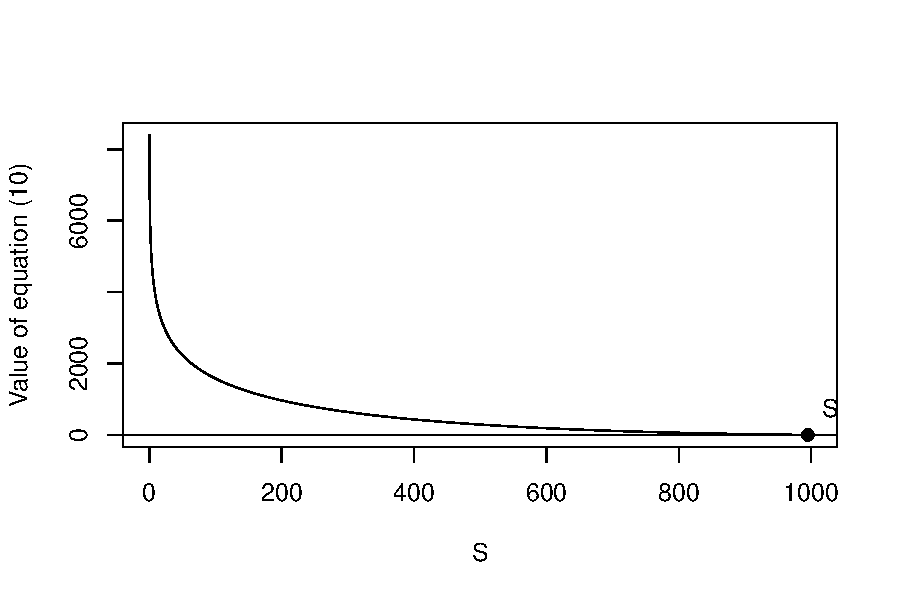
\includegraphics[width=\textwidth]{FIGS/course-01-KMK_final_size_0p8-1.pdf}
\end{center}
\end{frame}





\begin{frame}{$\R_0=2.4$}
  \begin{center}
    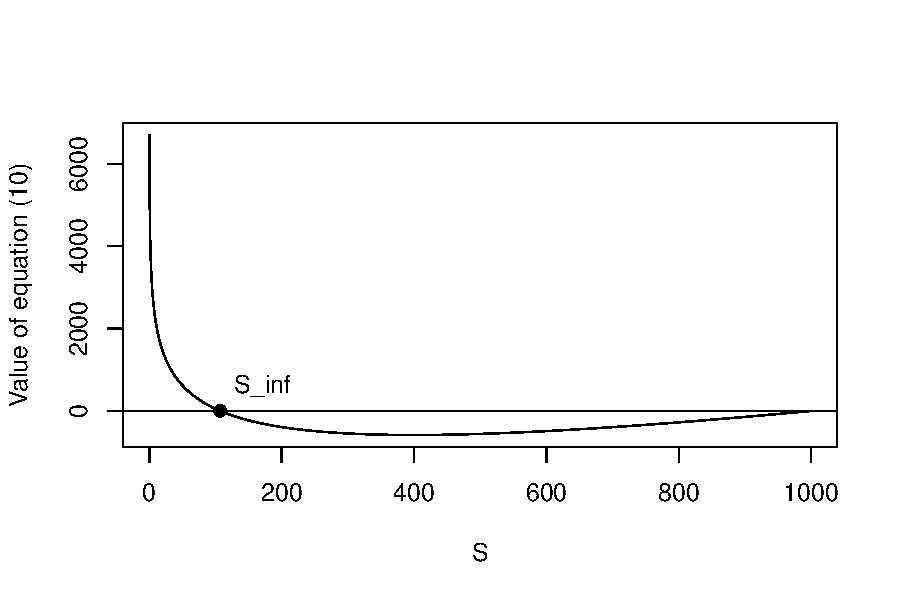
\includegraphics[width=\textwidth]{FIGS/course-01-KMK_final_size_2p5-1.pdf}
  \end{center}
\end{frame}

\begin{frame}[fragile]{A little nicer}
\begin{knitrout}
\definecolor{shadecolor}{rgb}{0.969, 0.969, 0.969}\color{fgcolor}\begin{kframe}
\begin{alltt}
\hldef{values} \hlkwb{=} \hlkwd{expand.grid}\hldef{(}
  \hlkwc{R_0} \hldef{=} \hlkwd{seq}\hldef{(}\hlnum{0.01}\hldef{,} \hlnum{3}\hldef{,} \hlkwc{by} \hldef{=} \hlnum{0.01}\hldef{),}
  \hlkwc{I0} \hldef{=} \hlkwd{seq}\hldef{(}\hlnum{1}\hldef{,} \hlnum{100}\hldef{,} \hlnum{1}\hldef{)}
\hldef{)}
\hldef{values}\hlopt{$}\hldef{S0} \hlkwb{=} \hldef{N0}\hlopt{-}\hldef{values}\hlopt{$}\hldef{I0}
\hldef{L} \hlkwb{=} \hlkwd{split}\hldef{(values,} \hlnum{1}\hlopt{:}\hlkwd{nrow}\hldef{(values))}
\hldef{values}\hlopt{$}\hldef{S_inf} \hlkwb{=} \hlkwd{sapply}\hldef{(}\hlkwc{X} \hldef{= L,} \hlkwc{FUN} \hldef{= final_size)}
\hldef{values}\hlopt{$}\hldef{final_size} \hlkwb{=} \hldef{values}\hlopt{$}\hldef{S0}\hlopt{-}\hldef{values}\hlopt{$}\hldef{S_inf}\hlopt{+}\hldef{values}\hlopt{$}\hldef{I0}
\hldef{values}\hlopt{$}\hldef{attack_rate} \hlkwb{=} \hldef{(values}\hlopt{$}\hldef{final_size} \hlopt{/} \hldef{N0)}\hlopt{*}\hlnum{100}

\hldef{p} \hlkwb{=} \hlkwd{levelplot}\hldef{(attack_rate} \hlopt{~} \hldef{R_0}\hlopt{*}\hldef{I0,} \hlkwc{data} \hldef{= values,}
              \hlkwc{xlab} \hldef{=} \hlkwd{TeX}\hldef{(}\hlsng{"$R_0$"}\hldef{),} \hlkwc{ylab} \hldef{=} \hlsng{"I(0)"}\hldef{,}
              \hlkwc{col.regions} \hldef{=} \hlkwd{viridis}\hldef{(}\hlnum{100}\hldef{))}
\hlkwd{print}\hldef{(p)}
\end{alltt}
\end{kframe}
\end{knitrout}
(requires \code{lattice}, \code{viridis} and \code{latex2exp} librairies)
\end{frame}

\begin{frame}{Attack rate (in \%)}
  \begin{center}
    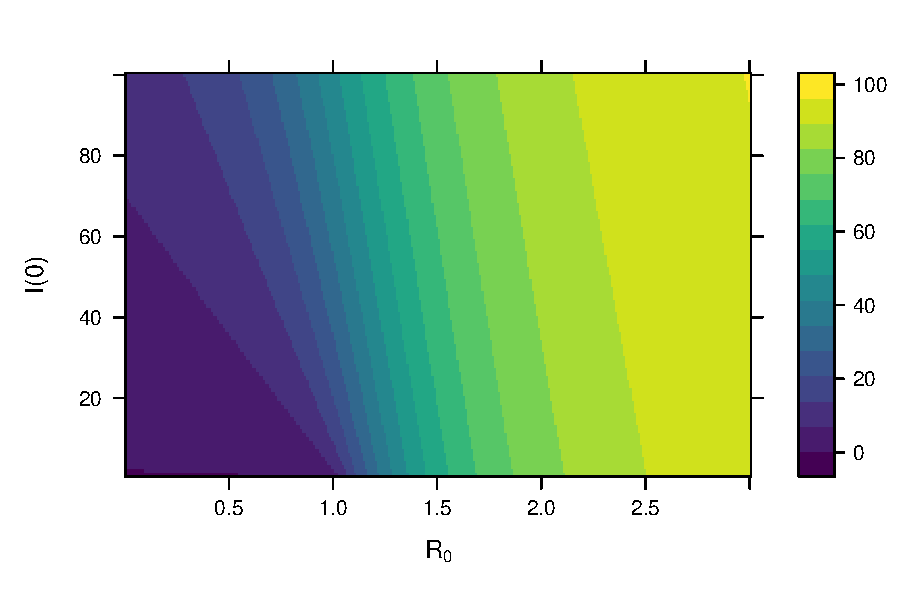
\includegraphics[width=0.9\textwidth]{FIGS/course-01-KMK_attack_rate-1.pdf}
  \end{center}
\end{frame}


%%%%%%%%%%%%%%%%%%%%%%%%%%%
%%%%%%%%%%%%%%%%%%%%%%%%%%%
\subsection{Herd immunity in KMK}
\newSubSectionSlide{FIGS-slides-admin/Gemini_Generated_Image_vqpscpvqpscpvqps.jpeg}


\begin{frame}{The simplest vaccination model}
To implement vaccination in KMK, assume that vaccination reduces the number of susceptibles
\vfill
Let total population be $N$ with $S_0$ initially susceptible
\vfill
Vaccinate a fraction $p\in[0,1]$ of susceptible individuals
\vfill
Original IC (for simplicity, $R(0)=0$)
\begin{equation}\label{eq:IC_KMK_novacc}
IC: (S(0),I(0),R(0)) = (S_0,I_0,0)
\end{equation}
Post-vaccination IC 
\begin{equation}\label{eq:IC_KMK_vacc}
IC: (S(0),I(0),R(0)) = ((1-p)S_0,I_0,pS_0)
\end{equation}
\end{frame}


\begin{frame}{Vaccination reproduction number}
  Without vaccination
  \begin{equation}\tag{\ref{eq:R0_KMK}}
    \R_0=\frac{\beta}{\gamma}S_0
  \end{equation}
  \vfill
  With vaccination, denoting $\R_{\text{v}}$ the reproduction number,
  \begin{equation}
    \R_{\text{v}} = \frac{\beta}{\gamma}(1-p)S_0
  \end{equation}
  \vfill
  Since $p\in[0,1]$, $\R_{\text{v}}\leq\R_0$
\end{frame}


\begin{frame}{Herd immunity}
  Therefore
  \begin{itemize}
    \item $\R_{\text{v}}<\R_0$ if $p>0$ 
    \item To control the disease, $\R_{\text{v}}$ must take a value less than 1
  \end{itemize}
  \vfill
To make $\R_{\text{v}}$ less than 1
  \begin{equation}\label{eq:herd_immunity}
    \R_{\text{v}}<1 \iff p> 1-\frac{1}{\R_0}
  \end{equation}
  \vfill
  By vaccinating a fraction $p>1-1/\R_0$ of the susceptible population, we thus are in a situation where an epidemic peak is precluded (or, at the very least, the final size is reduced)
  \vfill
  This is \defword{herd immunity}
\end{frame}


%%%%%%%%%%%%%%%%%%%%%%%
%%%%%%%%%%%%%%%%%%%%%%%
\subsection{The SLIAR model}
\newSubSectionSlide{FIGS-slides-admin/Gemini_Generated_Image_vqpscpvqpscpvqps.jpeg}

\maxFrameImage{FIGS/Arino-etal-SLIAR.png}

\begin{frame}
SIR is a little too simple for many diseases:
\vfill
\begin{itemize}
\item No incubation period
\vfill
\item A lot of infectious diseases (in particular respiratory) have mild and less mild forms depending on the patient
\end{itemize}
\vfill
$\implies$ model with SIR but also L(atent) and (A)symptomatic individuals, in which I are now symptomatic individuals
\end{frame}

\begin{frame}
\centering
\resizebox{\textwidth}{!}{
  \begin{tikzpicture}[%transform canvas={scale=1.3},
      auto,
      cloud/.style={minimum width={width("N-1")+2pt},
      draw, 
      ellipse,
      fill=gray!20}]
    \node [cloud, fill=green!90] (S) {$S$};
    \node [cloud, right=2cm of S, fill=red!30] (L) {$L$};
    \node [cloud, above right=of L, fill=red!90] (I) {$I$};
    \node [cloud, below right=of L, fill=red!60] (A) {$A$};
    \node [cloud, below right=of I, fill=blue!90] (R) {$R$};
    \node [cloud, right=1.5cm of I, draw=none, fill=none] (h1) {};
    %% Infections
    \path [line, very thick] (S) to node [midway, above] (TextNode) {$\beta S(I+\delta A)$} (L);
    \path [line, very thick] (L) to node [midway, above, sloped] (TextNode) {$p\kappa L$} (I);
    \path [line, very thick] (L) to node [midway, above, sloped] (TextNode) {$(1-p)\kappa L$} (A);
    \path [line, very thick] (I) to node [midway, above, sloped] (TextNode) {$f\alpha I$} (R);
    \path [line, very thick] (A) to node [midway, above, sloped] (TextNode) {$\eta A$} (R);
    \path [line, very thick] (I) to node [midway, above, sloped] (TextNode) {$(1-f)\alpha I$} (h1);
  \end{tikzpicture}
}
\end{frame}

\begin{frame}{Basic reproduction number \& Final size}
We find the basic reproduction number
\begin{equation}
\mathcal{R}_0=\beta
\left(
\frac{p}{\alpha}+\frac{\delta(1-p)}{\eta}
\right)S_0
=\frac{\beta\rho}{\alpha}S_0
\end{equation}
where 
\[
\rho = \alpha
\left(
\frac{p}{\alpha}+\frac{\delta(1-p)}{\eta}
\right)
\]
\vfill
The final size relation takes the form
\begin{equation}
S_0(\ln S_0-\ln S_\infty) =
\mathcal{R}_0(S_0-S_\infty)+\frac{\mathcal{R}_0I_0}{\rho}
\end{equation}
\end{frame}

\begin{frame}{Adding treatment}
\centering
\resizebox{0.8\textheight}{!}{
\def\horzskip{*2.75cm}
\def\vertskip{*1.5cm}
  \begin{tikzpicture}[%transform canvas={scale=1.3},
      auto,
      cloud/.style={minimum width={width("L\_T")+2pt},
      draw, 
      ellipse,
      fill=gray!20}]
    \node [cloud, fill=green!90] at (0,2\vertskip) (S) {$S$};
    \node [cloud, fill=red!30] at (1\horzskip,2\vertskip) (L) {$L$};
    \node [cloud, fill=red!90] at (2\horzskip,1\vertskip) (I) {$I$};
    \node [cloud, fill=red!60] at (2\horzskip,3\vertskip) (A) {$A$};
    \node [cloud, fill=blue!90] at (3\horzskip,0) (R) {$R$};
    \node [cloud, fill=green!90] at (0,-2\vertskip) (ST) {$S_T$};
    \node [cloud, fill=red!30] at (1\horzskip,-2\vertskip) (LT) {$L_T$};
    \node [cloud, fill=red!90] at (2\horzskip,-1\vertskip) (IT) {$I_T$};
    \node [cloud, fill=red!60] at (2\horzskip,-3\vertskip) (AT) {$A_T$};
    %% Flows untreated
    \path [line, very thick] (S) to node [midway, above] (TextNode) {$S\beta Q$} (L);
    \path [line, very thick] (L) to node [midway, above, sloped] (TextNode) {$p\kappa L$} (I);
    \path [line, very thick] (L) to node [midway, above, sloped] (TextNode) {$(1-p)\kappa L$} (A);
    \path [line, very thick] (I) to node [midway, above, sloped] (TextNode) {$f\alpha I$} (R);
    \path [line, very thick] (A) to node [midway, above, sloped] (TextNode) {$\eta A$} (R);
    %% Flows treated
    \path [line, very thick] (ST) to node [midway, above] (TextNode) {$\sigma_SS_T\beta Q$} (LT);
    \path [line, very thick] (LT) to node [midway, above, sloped] (TextNode) {$p\tau\kappa_T L_T$} (IT);
    \path [line, very thick] (LT) to node [midway, below, sloped] (TextNode) {$(1-p\tau)\kappa_T L_T$} (AT);
    \path [line, very thick] (IT) to node [midway, above, sloped] (TextNode) {$f_T\alpha_T I_T$} (R);
    \path [line, very thick] (AT) to node [midway, below, sloped] (TextNode) {$\eta_T A_T$} (R);
    %% Flow treatment
    \path [line, very thick, bend left=10] (LT) to node [midway, above, sloped] (TextNode) {$\theta_LL_T$} (L);
    \path [line, very thick, bend left=10] (L) to node [midway, above, sloped] (TextNode) {$\varphi_LL$} (LT);
    \path [line, very thick, bend left=10] (IT) to node [midway, above, sloped] (TextNode) {$\theta_II_T$} (I);
    \path [line, very thick, bend left=10] (I) to node [midway, above, sloped] (TextNode) {$\varphi_II$} (IT);
  \end{tikzpicture}
}
\end{frame}

\maxFrameImage{FIGS/Arino_etal-SLIAR-treatment-doses.png}
\maxFrameImage{FIGS/Arino_etal-SLIAR-treatment-cases.png}
\maxFrameImage{FIGS/Arino_etal-SLIAR-conclusions.png}
\maxFrameImage{FIGS/dedication-Fred-Brauer-169}

%%%%%%%%%%%%%%%%%%%%%%%
%%%%%%%%%%%%%%%%%%%%%%%
%%%%%%%%%%%%%%%%%%%%%%%
%%%%%%%%%%%%%%%%%%%%%%%
\subsection{Computing the final size more efficiently}
\newSubSectionSlide{FIGS-slides-admin/Gemini_Generated_Image_vqpscpvqpscpvqps.jpeg}

\maxFrameImage{FIGS/Arino-etal-final-size.png}

\begin{frame}{A method for computing $\mathcal{R}_0$ in epidemic models}
\bbullet This method is not universal! It works in a relatively large class of models, but not everywhere
\vfill
\bbullet If it doesn't work, the next generation matrix method does work, \textbf{but} should be considered only for obtaining the reproduction number, not to deduce LAS
\vfill
\bbullet Here, I change the notation in the paper, for convenience
\end{frame}

\begin{frame}{Standard form of the system}
Suppose system can be written in the form
\begin{subequations}\label{sys:SIR_general}
\begin{align}
\bS\pprime &= \mathbf{b}(\bS,\bI,\bR)-\bD\bS\beta(\bS,\bI,\bR)\bh\bI \label{sys:SIR_general_dS} \\
\bI\pprime &= \bPi\bD\bS\beta(\bS,\bI,\bR)\bh\bI-\mathbf{V}\bI \label{sys:SIR_general_dI} \\
\bR\pprime &= \mathbf{f}(\bS,\bI,\bR)+\mathbf{W}\bI \label{sys:SIR_general_dR}
\end{align}
\end{subequations}
\vfill
where $\bS\in\IR^m$, $\bI\in\IR^n$ and $\bR\in\IR^k$ are susceptible, infected and removed compartments, respectively
\vfill
IC are $\geq 0$ with at least one of the components of $\bI(0)$ positive
\end{frame}  


\begin{frame}
\begin{equation}\tag{\ref{sys:SIR_general_dS}}
\bS\pprime = \mathbf{b}(\bS,\bI,\bR)-\bD\bS\beta(\bS,\bI,\bR)\bh\bI
\end{equation}
\begin{itemize}
\item $\mathbf{b}:\IR_+^m\times\IR_+^n\times\IR_+^k\to\IR^m$ continuous function encoding recruitment and death of uninfected individuals
\item $\bD\in\IR^{m\times m}$ diagonal with diagonal entries $\sigma_i>0$ the relative susceptibilities of susceptible compartments, with convention that $\sigma_1=1$
\item Scalar valued function $\beta:\IR_+^m\times\IR_+^n\times\IR_+^k\to\IR_+$ represents infectivity, with, e.g., $\beta(\bS,\bI,\bR)=\beta$ for mass action
\item $\bh\in\IR^{n}$ row vector of relative horizontal transmissions
\end{itemize}
\end{frame}  


\begin{frame}
\begin{equation}\tag{\ref{sys:SIR_general_dI}}
\bI\pprime = \bPi\bD\bS\beta(\bS,\bI,\bR)\bh\bI-\mathbf{V}\bI
\end{equation}
\begin{itemize}
\item $\bPi\in\IR^{n\times m}$ has $(i,j)$ entry the fraction of individuals in $j^{\textrm{th}}$ susceptible compartment that enter $i^{\textrm{th}}$ infected compartment upon infection
\item $\bD\in\IR^{m\times m}$ diagonal with diagonal entries $\sigma_i>0$ the relative susceptibilities of susceptible compartments, with convention that $\sigma_1=1$
\item Scalar valued function $\beta:\IR_+^m\times\IR_+^n\times\IR_+^k\to\IR_+$ represents infectivity, with, e.g., $\beta(\bS,\bI,\bR)=\beta$ for mass action
\item $\bh\in\IR^{n}$ row vector of relative horizontal transmissions
\item $\mathbf{V}\in\IR^{n\times n}$ describes transitions between infected states and removals from these states due to recovery or death
\end{itemize}
\end{frame}  


\begin{frame}
\begin{equation}\tag{\ref{sys:SIR_general_dR}}
\bR\pprime = \mathbf{f}(\bS,\bI,\bR)+\mathbf{W}\bI
\end{equation}
\begin{itemize}
\item $\mathbf{f}:\IR_+^m\times\IR_+^n\times\IR_+^k\to \IR^k$ continuous function encoding flows into and out of removed compartments because of immunisation or similar processes
\item $\mathbf{W}\in\IR^{k\times n}$ has $(i,j)$ entry the rate at which individuals in the $j^{\textrm{th}}$ infected compartment move into the $i^{\textrm{th}}$ removed compartment
\end{itemize}
\end{frame}



\begin{frame}
Suppose $\bE_0$ is a locally stable disease-free equilibrium (DFE) of the system without disease, i.e., an EP of
\begin{align*}
\bS\pprime &= \mathbf{b}(\bS,\b0,\bR) \\
\bR\pprime &= \mathbf{f}(\bS,\b0,\bR) \\
\end{align*}

\begin{theorem}
Let
\begin{equation}\label{eq:R0_final_size_method}
\mathcal{R}_0 = 
\beta(\bS_0,\b0,\bR_0)
\bh\mathbf{V}^{-1}
\bPi\bD\bS_0
\end{equation}
\begin{itemize}
\item If $\mathcal{R}_0<1$, the DFE $\bE_0$ is a locally asymptotically stable EP of \eqref{sys:SIR_general}
\item If $\mathcal{R}_0>1$, the DFE $\bE_0$ of \eqref{sys:SIR_general} is unstable
\end{itemize}
\end{theorem}
\vfill
If no demography (epidemic model), then just $\R_0$, of course
\end{frame}  

\begin{frame}{Final size relations}
Assume no demography, then system should be writeable as
\begin{subequations}
\begin{align}
\bS\pprime &= -\bD\bS\beta(\bS,\bI,\bR)\bh\bI  \label{sys:SIR_epi_dS} \\
\bI\pprime &= \bPi\bD\bS\beta(\bS,\bI,\bR)\bh\bI-\mathbf{V}\bI 
\label{sys:SIR_epi_dI} \\
\bR\pprime &= \mathbf{W}\bI
\label{sys:SIR_epi_dR} 
\end{align}
\end{subequations}
\vfill
For $w(t)\in\IR_+^n$ continuous, define
$$
w_\infty = \lim_{t\to\infty}w(t)\quad\text{and}\quad
\hat{w}=\int_0^\infty w(t)\ dt
$$
\end{frame}  

\begin{frame}
Define the row vector 
\[
\IR^m\ni\bGamma
=(\Gamma_1,\ldots,\Gamma_m)=\beta(\bS_0,\b0,\bR_0)\bh\mathbf{V}^{-1}\bPi\bD
\]
then 
\[
\mathcal{R}_0=\bGamma\bS(0)
\]
\end{frame}  

\begin{frame}
Suppose incidence is mass action, i.e., $\beta(\bS,\bI,\bR)=\beta$ and $m>1$
\vfill
Then for $i=1,\ldots,m$, express $\bS_i(\infty)$ as a function of $\bS_1(\infty)$ using
$$
\bS_i(\infty)  = 
\bS_i(0) \left(
\frac{\bS_1(\infty)}{\bS_1(0)}
\right)^{\sigma_i/\sigma_1}
$$
then substitute into 
\begin{align*}
\frac{1}{\sigma_i}
\ln\left(\frac{\bS_i(0)}{\bS_i(\infty)}\right)
&=
\bGamma\bD^{-1}\left(\bS(0)-\bS(\infty)\right)
+\beta\bh\mathbf{V}^{-1}\bI(0) \\
&= 
\frac{1}{\sigma_1}
\ln\left(\frac{\bS_1(0)}{\bS_1(\infty)}\right)
\end{align*}
which is a final size relation for the general system when $\bS_i(0)>0$
\end{frame}  


\begin{frame}
If incidence is mass action and $m=1$ (only one susceptible compartment), reduces to the KMK form
\begin{equation}
\label{eq:final_size_m1}
\ln\left(
\frac{S_0}{S_\infty}
\right)
=\frac{\mathcal{R}_0}{S_0}
(S_0-S_\infty)+\beta\bh\mathbf{V}^{-1}\bI_0
\end{equation}
\end{frame}  


\begin{frame}
In the case of more general incidence functions, the final size relations are inequalities of the form, for $i=1,\ldots,m$,
$$
\ln\left(\frac{\bS_i(0)}{\bS_i(\infty)}\right)
\geq
\sigma_i\bGamma\bD^{-1}\left(\bS(0)-\bS(\infty)\right)
+\sigma_i\beta(K)\bh\mathbf{V}^{-1}\bI(0)
$$
where $K$ is the initial total population
\end{frame}  

%%%%%%%%%%%%%%%%%%%%
%%%%%%%%%%%%%%%%%%%%
\subsection{A variation on the SLIAR model}
\newSubSectionSlide{FIGS-slides-admin/Gemini_Generated_Image_vqpscpvqpscpvqps.jpeg}

\begin{frame}{The SLIAR model}
\bbullet Paper we have already seen: Arino, Brauer, PvdD, Watmough \& Wu. \href{http://dx.doi.org/10.1098/rsif.2006.0112}{Simple models for containment of a pandemic}, \emph{Journal of the Royal Society Interface} (2006)
\vfill
\bbullet However, suppose additionally that $L$ are also infectious
\end{frame}  

\begin{frame}
\centering
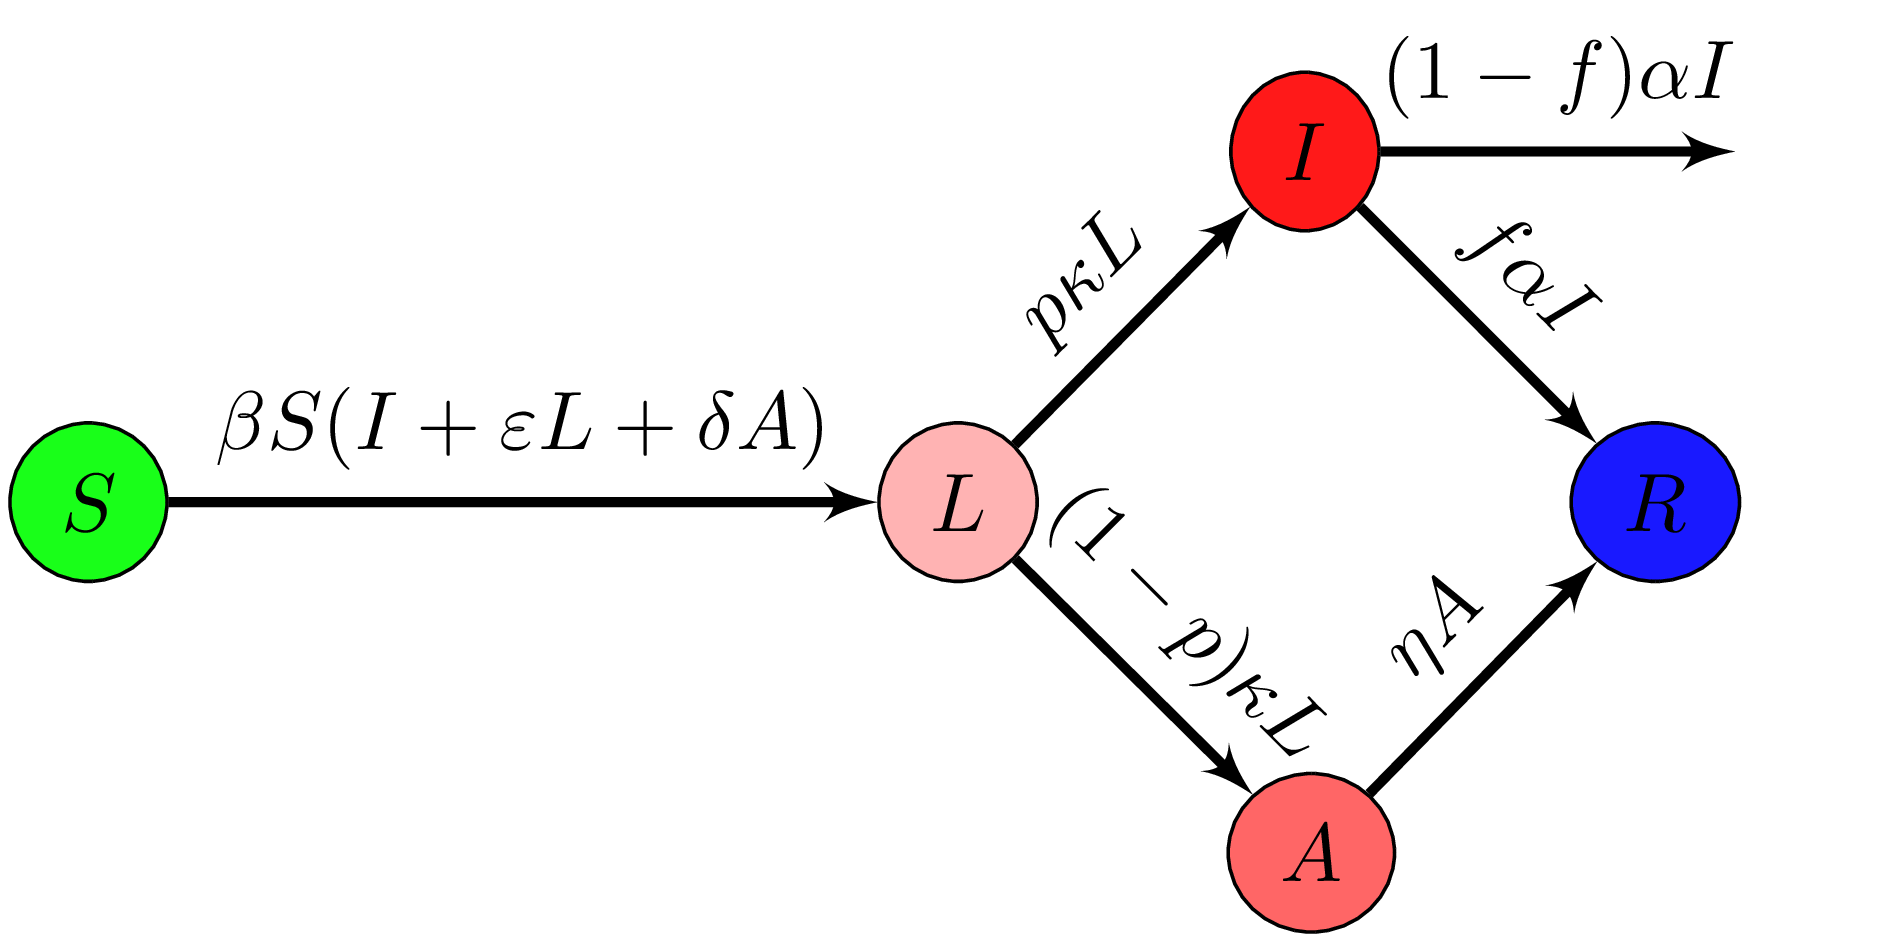
\includegraphics[width=\textwidth]{FIGS/SLIAR_infectiousL}
\end{frame}  


\begin{frame}
Here, $\bS=S$, $\bI=(L,I,A)^T$ and $\bR=R$, so $m=1$, $n=3$ and 
$$
\bh=[\varepsilon\; 1\; \delta],
\quad
\bD=1,
\quad 
\bPi
=\begin{pmatrix}
1 \\ 0 \\0
\end{pmatrix}
\quad\text{and}\quad
\mathbf{V}=
\begin{pmatrix}
\kappa & 0 & 0 \\
-p\kappa & \alpha & 0 \\
-(1-p)\kappa & 0 & \eta
\end{pmatrix}
$$
Incidence is mass action so $\beta(\bE_0)=\beta$ and thus
\begin{align*}
\mathcal{R}_0
&=
\beta\bh\mathbf{V}^{-1}\bPi\bD\bS_0 \\
&=
\beta\;
[\varepsilon\; 1\; \delta]
\begin{pmatrix}
1/\kappa & 0 & 0 \\
p/\alpha & 1/\alpha & 0 \\
(1-p)/\eta & 0 & 1/\eta
\end{pmatrix}
\begin{pmatrix}
1 \\ 0 \\0
\end{pmatrix}
S_0 \\
&=
\beta S_0\left(
\frac{\varepsilon}{\kappa}
+\frac{p}{\alpha}
+\frac{\delta(1-p)}{\eta}
\right)
\end{align*}
\end{frame}  

\begin{frame}
For final size, since $m=1$, we can use $\eqref{eq:final_size_m1}$:
\[
\ln\left(
\frac{S_0}{S_\infty}
\right)
=\frac{\mathcal{R}_0}{S_0}
(S_0-S_\infty)+\beta\bh\mathbf{V}^{-1}\bI_0
\]
\vfill
Suppose $\bI_0=(0,I_0,0)$, then
\[
\ln\left(
\frac{S_0}{S_\infty}
\right)
=\mathcal{R}_0\frac{S_0-S_\infty}{S_0}
+\frac{\beta}{\alpha}I_0
\]
\vfill
If $\bI_0=(L_0,I_0,A_0)$, then
\[
\ln\left(
\frac{S_0}{S_\infty}
\right)
=\mathcal{R}_0\frac{S_0-S_\infty}{S_0}
+\beta\left(
\frac{\varepsilon}{\kappa}
+\frac{p}{\alpha}
+\frac{\delta(1-p)}{\eta}
\right)L_0
+\frac{\beta\delta}{\eta}A_0
+\frac{\beta}{\alpha}I_0
\]
\end{frame}  



%%%%%%%%%%%%%%%%%%%%
%%%%%%%%%%%%%%%%%%%%
\subsection{A model with vaccination}
\newSubSectionSlide{FIGS-slides-admin/Gemini_Generated_Image_vqpscpvqpscpvqps.jpeg}

\begin{frame}{A model with vaccination}
\centering
\begin{tikzpicture}[auto, %node distance = 2cm, auto,
	cloud/.style={minimum width={width("N-1")+2pt},
		draw, ellipse,fill=gray!20}]
    \node [cloud, fill=green!90] (SU) {$S_U$};
    \node [cloud, below=2cmof SU, fill=green!90] (SV) {$S_V$};
    \node [cloud, right=3cm of SU, fill=red!30] (LU) {$L_U$};
    \node [cloud, right=3cm of SV, fill=red!30] (LV) {$L_V$};
	\node [cloud, right=of LU, fill=red!90] (IU) {$I_U$};
	\node [cloud, right=of LV, fill=red!90] (IV) {$I_V$};
	\node [cloud, below right=of IU, fill=blue!90] (R) {$R$};
    \node [cloud, above right=2cm of IU, draw=none, fill=none] (h1) {};
    \node [cloud, below right=2cm of IV, draw=none, fill=none] (h2) {};
	%% Infections
	\path [line, very thick] (SU) to node [midway, above] (TextNode) {$\beta S_U(I_U+\sigma_II_V)$} (LU);
	\path [line, very thick] (SV) to node [midway, above] (TextNode) {$\sigma_S\beta S_V(I_U+\sigma_II_V)$} (LV);
	\path [line, very thick] (LU) to node [midway, above, sloped] (TextNode) {$\kappa_U L_U$} (IU);
	\path [line, very thick] (LV) to node [midway, above, sloped] (TextNode) {$\kappa_V L_V$} (IV);
	\path [line, very thick] (IU) to node [midway, above, sloped] (TextNode) {$f_U\alpha_U I_U$} (R);
	\path [line, very thick] (IV) to node [midway, above, sloped] (TextNode) {$f_V\alpha_V I_V$} (R);
    \path [line, very thick] (IU) to node [midway, above, sloped] (TextNode) {$(1-f_U)\alpha_U I_U$} (h1);
    \path [line, very thick] (IV) to node [midway, below, sloped] (TextNode) {$(1-f_V)\alpha_V I_V$} (h2);
\end{tikzpicture}
\end{frame}  


\begin{frame}{A model with vaccination}
Fraction $\gamma$ of $S_0$ are vaccinated before the epidemic; vaccination reduces probability and duration of infection, infectiousness and reduces mortality
\begin{subequations}
\begin{align}
S_U\pprime &= -\beta S_U[I_U+\sigma_II_V] \\
S_V\pprime &= -\sigma_S\beta S_V[I_U+\sigma_II_V] \\
L_U\pprime &= \beta S_U[I_U+\sigma_II_V]-\kappa_UL_U\\
L_V\pprime &= \sigma_S\beta S_V[I_U+\sigma_II_V]-\kappa_VL_V \\
I_U\pprime &= \kappa_UL_U-\alpha_UI_U \\
I_V\pprime &= \kappa_VL_V-\alpha_VI_V \\
R\pprime &= f_U\alpha_UI_I+f_V\alpha_VI_V
\end{align}
\end{subequations}
with $S_U(0)=(1-\gamma)S_0$ and $S_V(0)=\gamma S_0$
\end{frame}  


\begin{frame}
Here, $m=2$, $n=4$,
\[
\bh = [0\;0\;1\;\sigma_I],\quad
\bD=\begin{pmatrix}
1 & 0 \\ 0 & \sigma_S
\end{pmatrix},\quad
\bPi=
\begin{pmatrix}
1 & 0 \\ 0 & 1 \\ 0 & 0 \\ 0 & 0
\end{pmatrix}
\]
and
\[
\mathbf{V}=
\begin{pmatrix}
\kappa_U & 0 & 0 & 0 \\
0 & \kappa_V & 0 & 0 \\
-\kappa_U & 0 & \alpha_U & 0 \\
0 & -\kappa_V & 0 & \alpha_V
\end{pmatrix}
\]
\end{frame}

\begin{frame}
So
\[
\bGamma=\left[
\frac{\beta}{\alpha_U}\; \frac{\sigma_I\sigma_S\beta}{\alpha_V}
\right],
\quad
\mathcal{R}_c = S_0\beta\left(
\frac{1-\gamma}{\alpha_U}+\frac{\sigma_I\sigma_S\gamma}{\alpha_V}
\right)
\]
and the final size relation is
\begin{multline*}
\ln\left(
\frac{(1-\gamma)S_U(0)}{S_U(\infty)}
\right)
= \\ 
\frac{\beta}{\alpha_U}[(1-\gamma)S_U(0)-S_U(\infty)] \\
+\frac{\sigma_I\beta}{\alpha_V}[\gamma S_V(0)-S_V(\infty)]+\frac{\beta}{\alpha_U}I_0 \\
\end{multline*}
\[
S_V(\infty) = \gamma S_U(0)\left(
\frac{S_U(\infty)}{(1-\gamma)S_0}
\right)^{\sigma_S}
\]
\end{frame}

%%%%%%%%%%%%%%%%%%%%
%%%%%%%%%%%%%%%%%%%%
\subsection{Antiviral resistance}
\newSubSectionSlide{FIGS-slides-admin/Gemini_Generated_Image_vqpscpvqpscpvqps.jpeg}

\maxFrameImage{FIGS/ArinoBowmanMoghadas.png}

\begin{frame}{Adapting treatment to counter emergence of resistance}
This work was undertaken at the request of the Public Health Agency of Canada during the pandemic preparadness phase prior to the 2009 p-H1N1 pandemic
\vfill
Problem: we have antivirals to use against influenza, either prophylactically or curatively. Using these antivirals may promote the emergence of antiviral-resistant strains. How do we minimise this risk?
\end{frame}


\begin{frame}
\centering
\resizebox{\textwidth}{!}{
  \begin{tikzpicture}[%transform canvas={scale=1.3},
      auto,
      cloud/.style={minimum width={width("N-1")+2pt},
      draw, 
      ellipse,
      fill=gray!20}]
    %% S
    \node [cloud, fill=green!90] at (0,0) (S) {$S$};
    %% Untreated, resistant
    \node [cloud, fill=red!90] at (3,1) (A_r) {$A_r$};
    \node [cloud, fill=red!60] at (3,-1) (I_rU) {$I_{rU}$};
    \node [cloud, fill=blue!60] at (6,0) (R_rU) {$R_{rU}$};
    %% Untreated, sensitive
    \node [cloud, fill=red!90] at (-3,1) (A) {$A$};
    \node [cloud, fill=red!60] at (-3,-1) (I_U) {$I_U$};
    \node [cloud, fill=blue!60] at (-6,0) (R_U) {$R_U$};
    %% Treated
    \node [cloud, fill=red!90] at (-1.5,-3) (I_T) {$I_T$};
    \node [cloud, fill=red!90] at (1.5,-3) (I_rT) {$I_{rT}$};
    \node [cloud, fill=red!90] at (0,-6) (I_Tr) {$I_{Tr}$};
    %% Resistance
    \node [cloud, fill=blue!60] at (-4.5,-3) (R_T) {$R_T$};
    \node [cloud, fill=blue!60] at (4.5,-3) (R_rT) {$R_{rT}$};
    \node [cloud, fill=blue!60] at (3,-6) (R_Tr) {$R_{Tr}$};
    %%
    %% Infections
    \path [line, very thick] (S) to node [midway,above,sloped] (TextNode) {$(1-p)fS$} (A);
    \path [line, very thick] (S) to node [midway,below,sloped] (TextNode) {$(1-q)pfS$} (I_U);
    \path [line, very thick] (S) to node [midway,above,sloped] (TextNode) {$(1-p)gS$} (A_r);
    \path [line, very thick] (S) to node [midway,below,sloped] (TextNode) {$(1-q)pgS$} (I_rU);
    \path [line, very thick] (S) to node [near end,above,sloped] (TextNode) {$qpfS$} (I_T);
    \path [line, very thick] (S) to node [midway,below,sloped] (TextNode) {$qpgS$} (I_rT);
    %% Removals
    \path [line, very thick] (A) to node [midway,below,sloped] (TextNode) {$\mu_AA$} (R_U);
    \path [line, very thick] (I_U) to node [midway,below,sloped] (TextNode) {$(d_U+\mu_U)I_U$} (R_U);
    \path [line, very thick] (A_r) to node [midway,below,sloped] (TextNode) {$\mu_AA_r$} (R_rU);
    \path [line, very thick] (I_rU) to node [midway,below,sloped] (TextNode) {$(d_{rU}+\mu_U)I_{rU}$} (R_rU);
    \path [line, very thick] (I_T) to node [midway,below,sloped] (TextNode) {$(d_T+\mu_T)I_T$} (R_T);
    \path [line, very thick] (I_rT) to node [midway,below,sloped] (TextNode) {$(d_{rU}+\mu_U)I_{rT}$} (R_rT);
    \path [line, very thick] (I_Tr) to node [midway,below,sloped] (TextNode) {$(d_{Ur}+\mu_U)I_{Tr}$} (R_Tr);
    %% I_T transitions
        \path [line, very thick] (I_T) to node [midway,below,sloped] (TextNode) {$\alpha I_T$} (I_Tr);
    \path [line, very thick] (I_Tr) to node [midway,below,sloped] (TextNode) {$\gamma I_{Tr}$} (I_rT);
  \end{tikzpicture}
}
\end{frame}

\begin{frame}
\centering
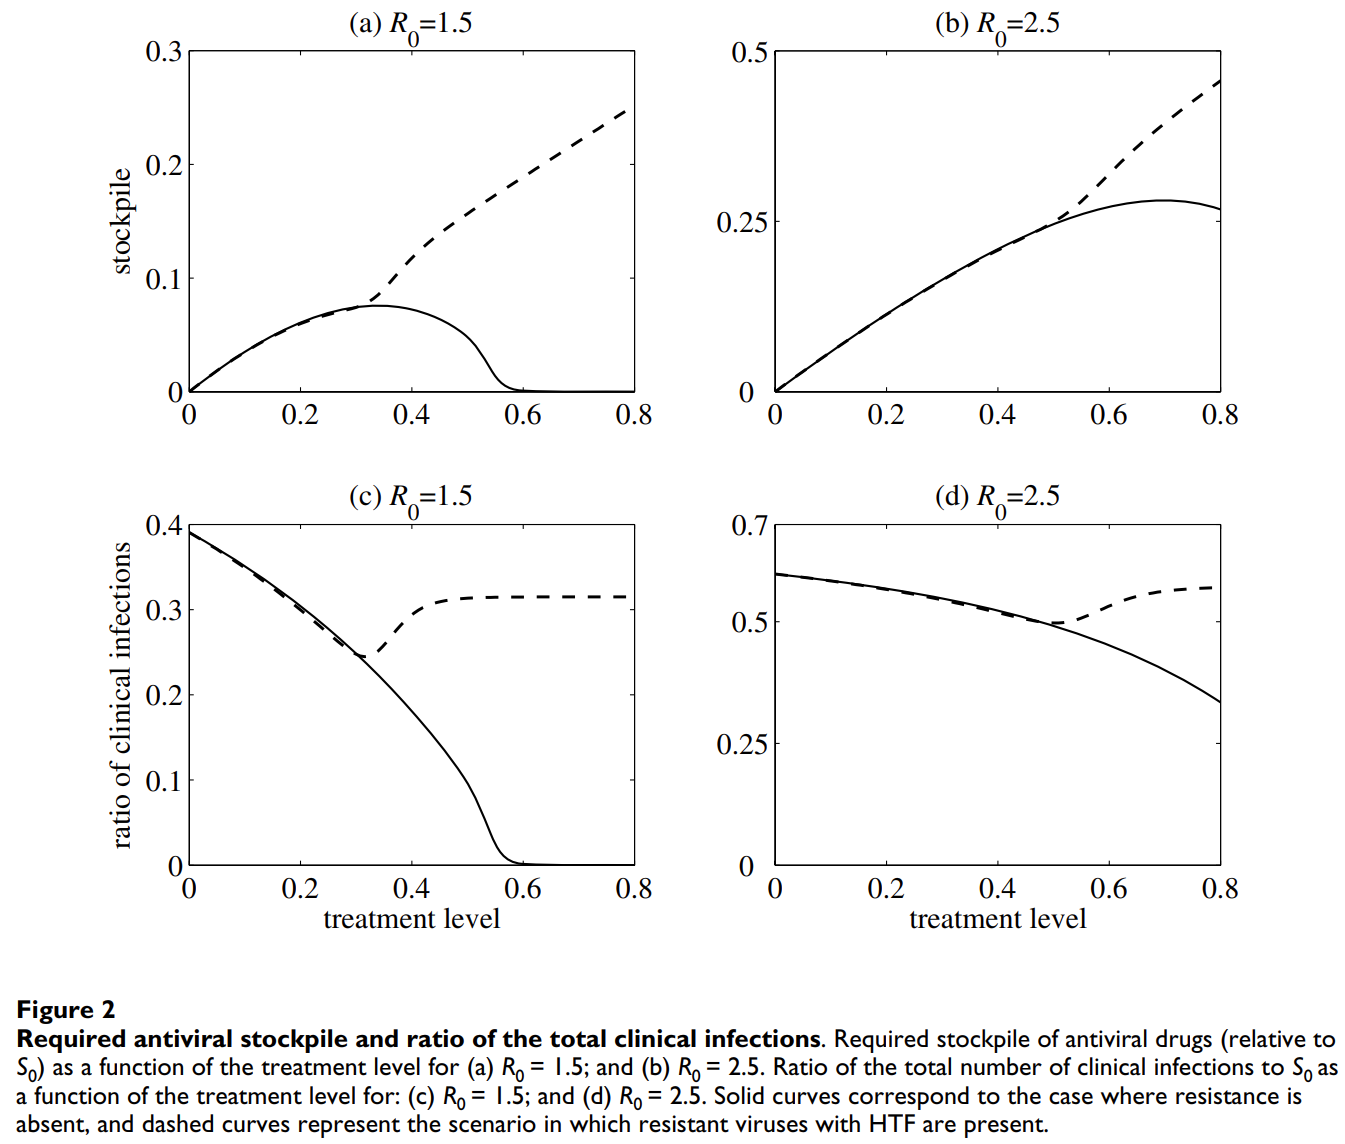
\includegraphics[height=\textheight]{FIGS/ABM-role-of-resistance}
\end{frame}

\begin{frame}
\centering
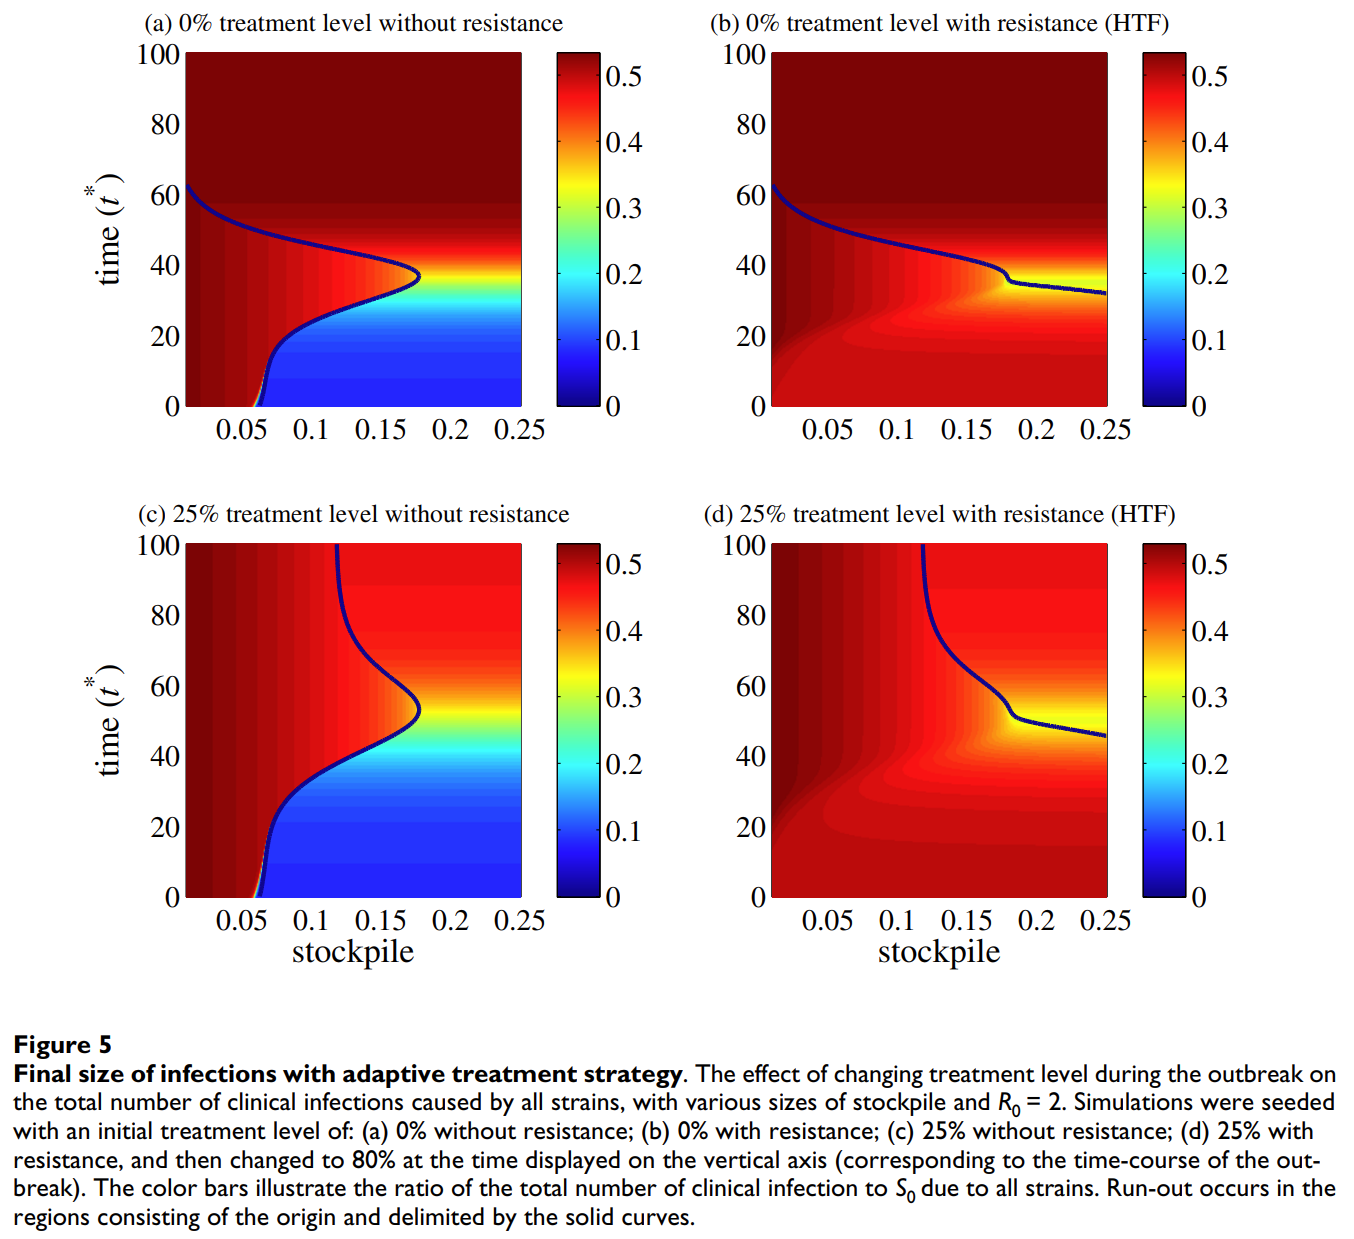
\includegraphics[height=\textheight]{FIGS/ABM-heatmaps}
\end{frame}

%%%%%%%%%%%%%%%%%%%
%%%%%%%%%%%%%%%%%%%
\subsection{A COVID-19 model}
\newSubSectionSlide{FIGS-slides-admin/Gemini_Generated_Image_vqpscpvqpscpvqps.jpeg}

\maxFrameImage{FIGS/ArinoPortet-2020.png}

\begin{frame}
Extends the SLIAR model to take into account non-exponentially distributed stage durations (see course 02)
\end{frame}

\begin{frame}{The original model (well, almost the first one)}
\centering
\def\horzskip{*2}
\def\vertskip{*2}
\begin{tikzpicture}[auto, %node distance = 2cm, auto,
	cloud/.style={minimum width={width("N-1")+2pt},
		draw, ellipse,fill=red!20}]
	\node [cloud] (S) at (0,0) {$S$};
	\node [cloud] (L1) at (1\horzskip,0) {$L_1$};
	\node [cloud] (L2) at (2\horzskip,0) {$L_2$};
	\node [cloud,fill=blue!20] (I1) at (3\horzskip,-1\vertskip) {$I_1$};
	\node [cloud] (A1) at (3\horzskip,1\vertskip) {$A_1$};
	\node [cloud,fill=blue!20] (I2) at (4\horzskip,-1\vertskip) {$I_2$};
	\node [cloud] (A2) at (4\horzskip,1\vertskip) {$A_2$};
	\node [cloud,fill=blue!20] (RI) at (5\horzskip,0) {$R_I$};
	\node [cloud] (RA) at (5\horzskip,1\vertskip) {$R_A$};
	\node [cloud,, fill=blue!20] (D) at (5\horzskip,-2\vertskip) {$D$};
	%% Infections
	\path [line, very thick] (S) to node [midway,above] (TextNode) {$\Phi S$} (L1);
	\path [line, very thick] (L1) to node [midway,above] (TextNode) {$\varepsilon L_1$} (L2);
	\path [line, very thick] (L2) to node [midway,below,sloped] (TextNode) {$(1-\pi)\varepsilon L_2$} (I1);
	\path [line, very thick] (L2) to node [midway,below,sloped] (TextNode) {$\pi\varepsilon L_2$} (A1);
	\path [line, very thick] (I1) to node [midway, above] (TextNode) {$\gamma I_1$} (I2);
	\path [line, very thick] (A1) to node [midway, above] (TextNode) {$\gamma A_1$} (A2);
	\path [line, very thick] (I2) to node [midway,above,sloped] (TextNode) {$(1-\delta)\gamma I_2$} (RI);
	\path [line, very thick] (A2) to node [midway, above] (TextNode) {$\gamma A_2$} (RA);
	\path [line, very thick] (I2) to node [midway,below,sloped] (TextNode) {$\delta\gamma I_2$} (D);
\end{tikzpicture}
\end{frame}


\begin{frame}{Reinterpreting terms}
Here $D$ stands for \emph{detected}, $U$ is \emph{undetected}
\vfill
\centering
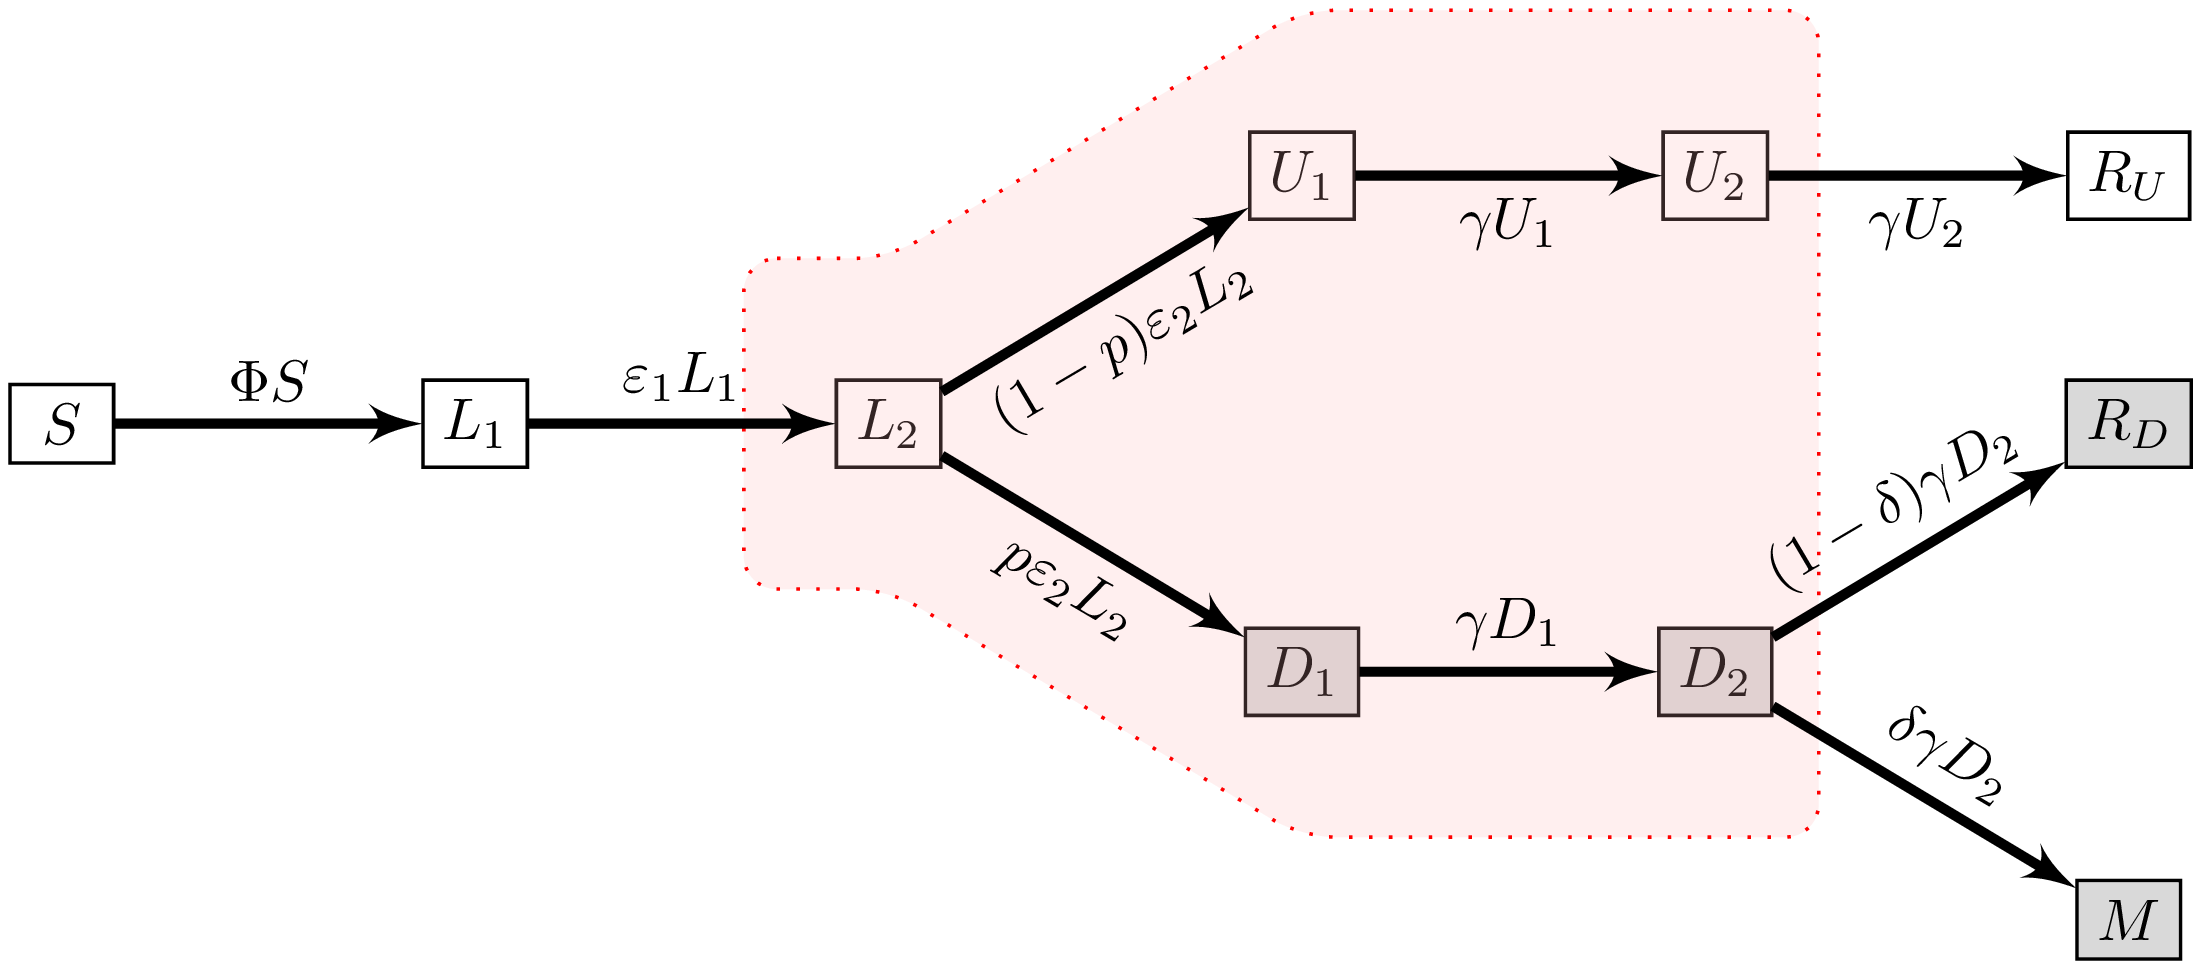
\includegraphics[width=\textwidth]{FIGS/figure_SLDURM_base_model_with_different_epsilon_and_infectious_compartments}
\end{frame}

\begin{frame}{Working out when the first COVID-19 case occurred}
\bbullet Details of emergence and precise timeline before amplification started unknown
\vfill
\bbullet Amplification in Wuhan
\begin{itemize}
\item Cluster of pneumonia cases mostly related to the Huanan Seafood Market
\item 27 December 2019: first report to local government
\item 31 December 2019: publication
\item 8 January 2020: identification of SARS-CoV-2 as causative agent
\item $\sim$ 23 January 2020: lockdown Wuhan and Hubei province + face mask mandates
\end{itemize}
\vfill
\bbullet By 2020-01-29, virus in all provinces of mainland CHN
\end{frame}


\begin{frame}{Evidence of earlier spread}
\bbullet Report to Wuhan authorities on 27 December 2019
\vfill
\bbullet First export detections in Thailand and Japan on 13 and 16 January 2020 (with actual importations on 8 and 6 January)
\vfill
$\implies$ amplification must have been occuring for a while longer
\vfill
\bbullet France: sample taken from 42-year-old male (last foreign travel to Algeria in August 2019) who presented to ICU on 27 December 2019
\vfill
\bbullet Retrospective studies in United Kingdom and Italy also showed undetected COVID-19 cases in prepandemic period
\end{frame}

\begin{frame}{Untangling the first case issue}
\bbullet Robert, Rossman \& Jaric. Dating first cases of COVID-19. \emph{PLoS Pathogens} (2021)

Find likely timing of first case of COVID-19 in China as November 17 (95\% CI October 4)
\vfill
\bbullet Pekar, Worobey, Moshiri, Scheffler \& Wertheim. Timing the SARS-CoV-2 index case in Hubei province. \emph{Science} (2021)

Period between mid-October and mid-November 2019 is plausible interval when the first case of SARS-CoV-2 emerged in Hubei province
\vfill
Important when trying to understand global spread, so let me illustrate with the model I used, taking into account model evolution since
\end{frame}

\begin{frame}{Back-calculating the start of spread (example of China)}
Cumulative confirmed case counts in China as reported to WHO was $c=547$ cases on $t_c=\textrm{2020-01-22}$
\vfill
Let $u$ be a point in parameter space. Solve ODE numerically over $[0,t]$, with $S(0)$ the population of China, $L_1(0)=1$ and other state variables 0. This gives a solution $x(t,t_0=0,u)$
\vfill
Extracting $L_2(t,t_0=0,u)$ from this solution, obtain cumulative number of new detections as
\[
C(t) = \int_{t_0=0}^{t} p\varepsilon_2 L_2(s,t_0,u)\ ds
\]
\vfill
Let $t^\star$ be s.t. $C(t^\star)=547$; then $t_i=\textrm{2020-01-22}-t^\star$
\end{frame}

\begin{frame}
\centering
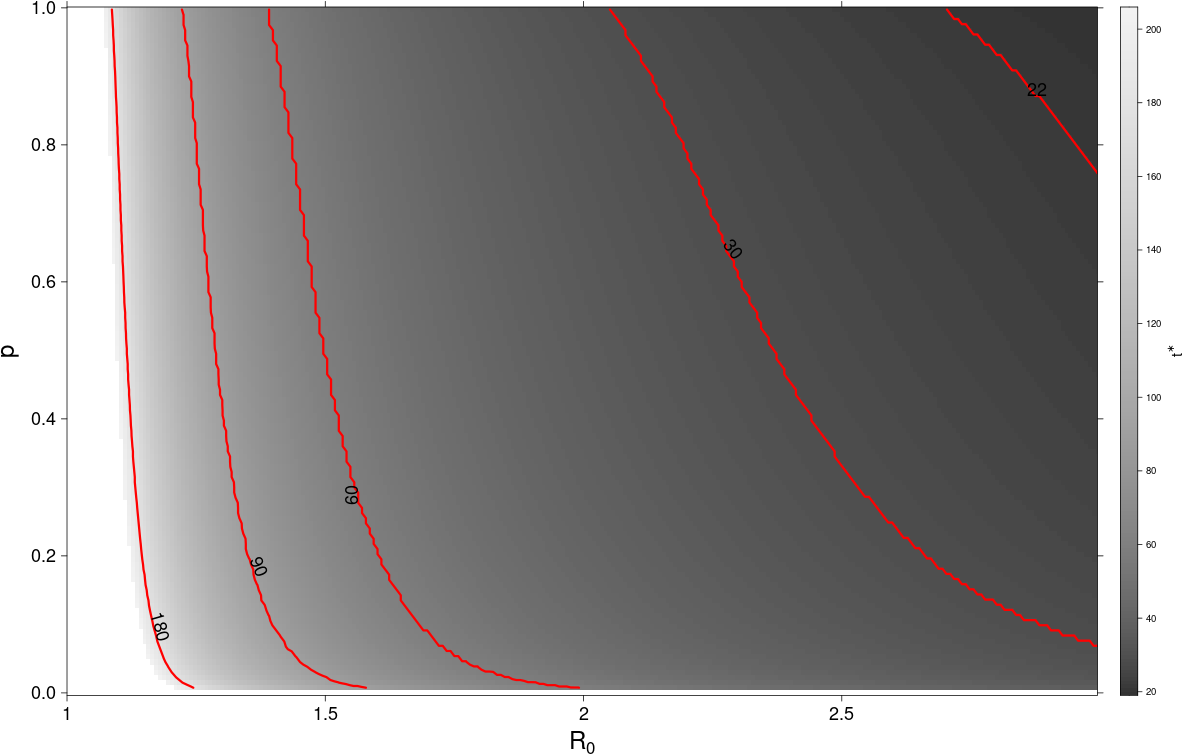
\includegraphics[width=\textwidth]{FIGS/start_time_vs_R0_and_p.png}
\end{frame}




%%%%%%%%%%%%%%%%%%%%
%%%%%%%%%%%%%%%%%%%%
%%%%%%%%%%%%%%%%%%%%
%%%%%%%%%%%%%%%%%%%%
\section{Endemic SIRS-type models with demography}
\newSectionSlide{FIGS-slides-admin/Gemini_Generated_Image_vqpscpvqpscpvqps.jpeg}

%%%%%%%%%%%%%%%%%%%%
%%%%%%%%%%%%%%%%%%%%
\subsection{The SIRS model(s)}
\begin{frame}{Two potential variations on the Kermack-McKendrick model}
\bbullet Add \emph{vital dynamics}, i.e., consider demographic processes
\vfill
\bbullet Individuals do not die from the disease; after recovering, individuals are \emph{immune} from infection for some time
\vfill
\bbullet We can of course combine both!
\end{frame}

\begin{frame}{Potential variations}
\def\skip{*1.5}
\def\yskip{*-2.5}
\begin{center}
  \begin{tikzpicture}[scale=1.15, transform shape]
    %% Regular nodes
    \node [circle, fill=green!50, text=black] at (0\skip,0) (S1) {$S$};
    \node [circle, fill=red!90, text=black] at (1\skip,0) (I1) {$I$};
    \node [circle, fill=blue!90, text=black] at (2\skip,0) (R1) {$R$};
    %% Fake nodes for arrows
    \node [left=1cm of S1] (birth1) {};
    \node [below=0.5cm of S1] (dS1) {};
    \node [below=0.5cm of I1] (dI1) {};
    \node [below=0.5cm of R1] (dR1) {};
    %% Flows
    \path [line, very thick] (birth1) to node [midway, above] (TextNode) {$b(N)$} (S1);
    \path [line, very thick] (S1) to node [midway, right] (TextNode) {$dS$} (dS1);
    \path [line, very thick] (I1) to node [midway, right] (TextNode) {$dI$} (dI1);
    \path [line, very thick] (R1) to node [midway, right] (TextNode) {$dR$} (dR1);
    \path [line, very thick] (S1) to node [midway, above] (TextNode) {$\beta SI$} (I1);
    \path [line, very thick] (I1) to node [midway, above] (TextNode) {$\gamma I$} (R1);
    \node [circle, fill=green!50, text=black] at (0,1\yskip) (S2) {$S$};
    \node [circle, fill=red!90, text=black] at (1\skip,1\yskip) (I2) {$I$};
    \node [circle, fill=blue!90, text=black] at (2\skip,1\yskip) (R2) {$R$};
    %% Flows
    \path [line, very thick] (S2) to node [midway, above] (TextNode) {$\beta SI$} (I2);
    \path [line, very thick] (I2) to node [midway, above] (TextNode) {$\gamma I$} (R2);
    \draw [>=latex,->, thick, rounded corners] (R2) -- (2\skip,0.75\yskip) -- (0,0.75\yskip) node[sloped, midway, above] {$\nu R$} -- (S2);
    %% Regular nodes
    \node [circle, fill=green!50, text=black] at (0\skip,2\yskip) (S3) {$S$};
    \node [circle, fill=red!90, text=black] at (1\skip,2\yskip) (I3) {$I$};
    \node [circle, fill=blue!90, text=black] at (2\skip,2\yskip) (R3) {$R$};
    %% Fake nodes for arrows
    \node [left=1cm of S3] (birth3) {};
    \node [below=0.5cm of S3] (dS3) {};
    \node [below=0.5cm of I3] (dI3) {};
    \node [below=0.5cm of R3] (dR3) {};
    %% Flows
    \path [line, very thick] (birth3) to node [midway, above] (TextNode) {$b(N)$} (S3);
    \path [line, very thick] (S3) to node [midway, right] (TextNode) {$dS$} (dS3);
    \path [line, very thick] (I3) to node [midway, right] (TextNode) {$dI$} (dI3);
    \path [line, very thick] (R3) to node [midway, right] (TextNode) {$dR$} (dR3);
    \path [line, very thick] (S3) to node [midway, above] (TextNode) {$\beta SI$} (I3);
    \path [line, very thick] (I3) to node [midway, above] (TextNode) {$\gamma I$} (R3);
    \draw [>=latex,->, thick, rounded corners] (R3) -- (2\skip,1.75\yskip) -- (0,1.75\yskip) node[sloped, midway, above] {$\nu R$} -- (S3);
  \end{tikzpicture}    
\end{center}
\end{frame}


\begin{frame}{The model}
\begin{minipage}{0.25\textwidth}
  \def\skip{*-1.5}
  \begin{tikzpicture}[scale=1, transform shape]
    %% Regular nodes
    \node [circle, fill=green!50, text=black] at (0,0) (S) {$S$};
    \node [circle, fill=red!90, text=black] at (0,1\skip) (I) {$I$};
    \node [circle, fill=blue!90, text=black] at (0,2\skip) (R) {$R$};
    %% Fake nodes for arrows
    \node [above=1cm of S] (birth) {};
    \node [left=0.5cm of S] (dS) {};
    \node [left=0.5cm of I] (dI) {};
    \node [left=0.5cm of R] (dR) {};
    %% Flows
    \path [line, very thick] (birth) to node [midway, left] (TextNode) {$b(N)$} (S);
    \path [line, very thick] (S) to node [midway, above] (TextNode) {$dS$} (dS);
    \path [line, very thick] (I) to node [midway, above] (TextNode) {$dI$} (dI);
    \path [line, very thick] (R) to node [midway, above] (TextNode) {$dR$} (dR);
    \path [line, very thick] (S) to node [midway, right] (TextNode) {$\beta SI$} (I);
    \path [line, very thick] (I) to node [midway, right] (TextNode) {$\gamma I$} (R);
    \draw [>=latex,->, thick, rounded corners] (R) -- (0.75,2\skip) -- (0.75,0) node[midway, right] {$\nu R$} -- (S);
  \end{tikzpicture}    
\end{minipage}
\begin{minipage}{0.7\textwidth}
  \begin{subequations} \label{sys:SIRS_base}
  \begin{align}
    S\pprime &= b(N)+\nu R-dS-\beta SI \label{sys:SIRS_base_dS} \\
    I\pprime &= \beta SI-(d+\gamma) I \label{sys:SIRS_base_dI} \\
    R\pprime &= \gamma I-(d+\nu)R \label{sys:SIRS_base_dR}
  \end{align}    
  \end{subequations}
  \vskip1cm
  Consider the initial value problem consisting in \eqref{sys:SIRS_base} to which we adjoin initial conditions $S(0)=S_0\geq 0$, $I(0)=I_0\geq 0$ and $R(0)=R_0\geq 0$
  \vskip1cm
  Typically, we assume $N_0=S_0+I_0+R_0>0$ to avoid a trivial case
  \end{minipage}
\end{frame}

\begin{frame}{Birth and death are \emph{relative}}
  Remark that the notions of \emph{birth} and \emph{death} are relative to the population under consideration
  \vfill
  E.g., consider a model for human immunodeficiency virus (HIV) in an at-risk population of intravenous drug users. Then
  \begin{itemize}
    \item birth is the moment the at-risk behaviour starts 
    \item death is the moment the at-risk behaviour stops,  whether from ``real death'' or because the individual stops using drugs
  \end{itemize}
\end{frame}

\begin{frame}{Choosing a form for demography}
Before we proceed with the analysis proper, we must discuss the nature of the assumptions on demography
\vfill
To do this, we consider the behaviour of the total population 
\[
N(t)=S(t)+I(t)+R(t)
\]
\end{frame}

\begin{frame}{Behaviour of the total population}
Summing the equations in \eqref{sys:SIRS_base}
\begin{equation}\label{eq:total_pop_general}
N\pprime=b(N)-dN
\end{equation}
\vfill
There are three common ways to define $b(N)$ in \eqref{eq:total_pop_general}
\begin{enumerate}
\item $b(N)=b$
\item $b(N)=bN$
\item $b(N)=bN-cN^2$
\end{enumerate}
\vfill
Case 3 leads to logistic dynamics of the total population and is not discussed here
\end{frame}


\begin{frame}{Case of a birth rate constant \emph{per capita}}
If $b(N)=bN$, then birth in \eqref{eq:total_pop_general} satisfies $N'/N=b$; we say that birth is \defword{constant \emph{per capita}}
\vfill
In this case, \eqref{eq:total_pop_general} takes the form
\[
N\pprime=bN-dN=(b-d)N
\]
with initial condition $N(0)=N_0$
\vfill
The solution to this scalar autonomous ODE is easy
\[
N(t)=N_0e^{(b-d)t},\quad t\geq 0
\]
Thus there are 3 possibilities:
\begin{itemize}
  \item if $b>d$, $N(t)\to\infty$, the total population explodes 
  \item if $b=d$, $N(t)\equiv N_0$, the total population remains constant 
  \item if $b<d$, $N(t)\to 0$, the total population collapses
\end{itemize}
\end{frame}

\begin{frame}{From now on, assume $b(N)=b$}
\bbullet We want a reasonable case, we could therefore suppose that $b(N)=d$, which would lead to a constant total population
\vfill
\bbullet However, this is a little reductive, so we choose instead $b(N)=b$, which, we will see, works as well even though it can initially be thought of as not being very realistic
\end{frame}


\begin{frame}{The model (for good this time)}
\begin{minipage}{0.25\textwidth}
  \def\skip{*-1.5}
  \begin{tikzpicture}[scale=1, transform shape]
    %% Regular nodes
    \node [circle, fill=green!50, text=black] at (0,0) (S) {$S$};
    \node [circle, fill=red!90, text=black] at (0,1\skip) (I) {$I$};
    \node [circle, fill=blue!90, text=black] at (0,2\skip) (R) {$R$};
    %% Fake nodes for arrows
    \node [above=1cm of S] (birth) {};
    \node [left=0.5cm of S] (dS) {};
    \node [left=0.5cm of I] (dI) {};
    \node [left=0.5cm of R] (dR) {};
    %% Flows
    \path [line, very thick] (birth) to node [midway, left] (TextNode) {$b$} (S);
    \path [line, very thick] (S) to node [midway, above] (TextNode) {$dS$} (dS);
    \path [line, very thick] (I) to node [midway, above] (TextNode) {$dI$} (dI);
    \path [line, very thick] (R) to node [midway, above] (TextNode) {$dR$} (dR);
    \path [line, very thick] (S) to node [midway, right] (TextNode) {$\beta SI$} (I);
    \path [line, very thick] (I) to node [midway, right] (TextNode) {$\gamma I$} (R);
    \draw [>=latex,->, thick, rounded corners] (R) -- (0.75,2\skip) -- (0.75,0) node[midway, right] {$\nu R$} -- (S);
  \end{tikzpicture}    
\end{minipage}
\begin{minipage}{0.7\textwidth}
  \begin{subequations} \label{sys:SIRS}
  \begin{align}
    S\pprime &= b+\nu R-dS-\beta SI \label{sys:SIRS_dS} \\
    I\pprime &= \beta SI-(d+\gamma) I \label{sys:SIRS_dI} \\
    R\pprime &= \gamma I-(d+\nu)R \label{sys:SIRS_dR}
  \end{align}    
  \end{subequations}
  \vskip1cm
  Consider the initial value problem consisting in \eqref{sys:SIRS} to which we adjoin initial conditions $S(0)=S_0\geq 0$, $I(0)=I_0\geq 0$ and $R(0)=R_0\geq 0$
  \vskip1cm
  Typically, we assume $N_0=S_0+I_0+R_0>0$ to avoid a trivial case
  \end{minipage}
\end{frame}


%%%%%%%%%%%%%%%%%%%%%%
%%%%%%%%%%%%%%%%%%%%%%
%%%%%%%%%%%%%%%%%%%%%%
%%%%%%%%%%%%%%%%%%%%%%
\subsection{Mathematical analysis of the SIRS model}
\newSubSectionSlide{FIGS-slides-admin/Gemini_Generated_Image_vqpscpvqpscpvqps.jpeg}


\begin{frame}{Is the system well-posed?} 
For an ODE epidemiological model
\vfill
\bbullet Do solutions to \eqref{sys:SIRS} exist and are they unique?
\vfill
\bbullet Is the positive cone invariant under the flow of \eqref{sys:SIRS}?
\vfill
\bbullet Are solutions to \eqref{sys:SIRS} bounded?
Some models have unbounded solutions but they are rare and will need to be considered specifically
\end{frame}

\begin{frame}{Solutions exist and are unique}
\bbullet The vector field is always $C^1$, implying that solutions exist and are unique
\vfill
If we had instead considered an incidence of the form $f(S,I,N)=\beta SI/N$ and, say, demography with $b(N)=bN$, then some discussion might have been needed if $b<d$
\end{frame}


\begin{frame}{Invariance of $\IR_+^3$ under the flow (1)}
Let us start by assuming that $I(0)=I_0=0$. Then \eqref{sys:SIRS_dI} remains $I\pprime=0$, meaning that the $SR$-plane (i.e., the set $\{I=0\}$) is positively invariant under the flow of \eqref{sys:SIRS}
\vfill
On that plane, \eqref{sys:SIRS} reduce to
\begin{subequations}\label{sys:SIRS_on_Ieq0}
\begin{align}
S\pprime &= b+\nu R-dS \\
R\pprime &= -(d+\nu)R
\end{align}    
\end{subequations}
\vfill
$\implies$ a solution with $I_0>0$ cannot enter the plane $\{I=0\}$. Indeed, suppose that $I_0>0$ but $\exists t_\star>0$ such that $I(t_\star)=0$. Then at $(S(t_\star),I(t_\star)=0,R(t_\star))$, there are two solutions to \eqref{sys:SIRS}: the one we just generated as well as the one governed by \eqref{sys:SIRS_on_Ieq0}
\vfill
This contradicts uniqueness of solutions to \eqref{sys:SIRS}
\end{frame}

\begin{frame}{Invariance of $\IR_+^3$ under the flow (2)} 
We saw that $I(t)>0$ if $I(0)>0$
\vfill
Suppose now that $S=0$. Equation \eqref{sys:SIRS_dS} is then
$$
S\pprime = b+\nu R>0
$$
\vfill
So if $S(0)=S_0>0$, then $S(t)>0$ for all $t$. If, on the other hand, $S_0=0$, then $S(t)>0$ for $t>0$ small; from what we just saw, this is then also true for all $t>0$
\vfill
We say the vector field points \emph{inward}
\vfill
$\implies$ $S$ cannot become zero
\vfill
Do the same for $R$
\end{frame}

\begin{frame}{To summarise, for invariance}
For simplicity, denote $\IR^\star=\IR\setminus\{0\}$
\vfill
\bbullet If $(S(0),I(0),R(0))\in\IR_+\times \IR_+^\star\times\IR_+$, then $\forall t>0$,
\[
(S(t),I(t),R(t))\in(\IR_+^\star)^3
\]
\vfill
\bbullet If $(S(0),I(0),R(0))\in\IR_+\times\{0\}\times\IR_+$, then $\forall t\geq 0$, 
\[
(S(t),I(t),R(t))\in\IR_+^\star\times\{0\}\times\IR_+
\]
\vfill
The model is therefore satisfactory in that it does not allow solutions to become negative
\end{frame}

\begin{frame}{Remark -- Know your audience} 
This reasoning has its place in an MSc of PhD manuscript: you need to demonstrate that you know what to do and how to do it
\vfill
In a research paper, this is not really necessary and actually often superfluous; the statement \emph{it is easy to show that solutions exist uniquely and that the positive orthant is invariant under the flow of the system} is typically sufficient
\vfill
(However, be sure to cover your bases: don't show the proof in the paper but have it in your notes.. \emph{it is easy to show} can be a dangerous statement if it is not easy...)
\end{frame}


\begin{frame}{The total population is asymptotically constant}
Since $b(N)=b$, the total population equation \eqref{eq:total_pop_general} takes the form
\[
N\pprime = b-dN
\]
This equation has a unique equilbrium $N^\star=b/d$ and it is very easy to check that this equilibrium is GAS: this is a scalar autonomous equation, so solutions are monotone; they increase to $N^\star$ if $N_0<N^\star$ and decrease to $N^\star$ if $N_0>N^\star$
\vfill
So we can work at the limit $N^\star$ where $R=N^\star-(S+I)$ and thus drop the equation for $R$
\end{frame}


\begin{frame}{Boundedness}
It follows from what we just saw that the positive cone $\IR_+^3$ is (positively) invariant under the flow of \eqref{sys:SIRS}
\vfill
Since $N(t)\to N^\star$, we deduce that solutions of \eqref{sys:SIRS} are bounded
\end{frame}


\begin{frame}{Seeking equilibria}
We seek $S=S^\star, I=I^\star, R=R^\star$ such that
\begin{subequations} \label{sys:SIRS_EP}
\begin{align}
0 &= b+\nu R-dS-\beta SI \label{sys:SIRS_EP_dS} \\
0 &= \beta SI-(d+\gamma) I \label{sys:SIRS_EP_dI} \\
0 &= \gamma I-(d+\nu)R \label{sys:SIRS_EP_dR}
\end{align}    
\end{subequations}
\vfill
From \eqref{sys:SIRS_EP_dI}, either $I^\star=0$ or $\beta S-(d+\gamma)=0$, i.e., $S^\star=(d+\gamma)/\beta$
\vfill
When $I^\star=0$, substituting $I^\star=0$ into \eqref{sys:SIRS_EP_dR} implies that $R^\star=0$ and, in turn, substituting $I^\star=R^\star=0$ into \eqref{sys:SIRS_EP_dR} gives $S^\star=b/d$. This gives the disease-free equilibrium (DFE)
\begin{equation}\label{eq:SIRS_DFE}
\bE_0:=(S^\star,I^\star,R^\star)=
\left(\frac bd, 0, 0\right)
\end{equation}
\vfill
We return to $S^\star=(d+\gamma)/\beta$ in a while
\end{frame}



\begin{frame}{Classic method for computing $\R_0$}
$\R_0$ is the surface in parameter space where the DFE loses its LAS
\vfill
To find $\R_0$, we therefore study the LAS of the DFE
\vfill
In an arbitrary $(S,I,R)$, the Jacobian matrix of \eqref{sys:SIRS} takes the form
\begin{equation}
\label{eq:SIRS_Jacobian}
J_{(S,I,R)} =
\begin{pmatrix}
-d-\beta I & -\beta S & \nu \\
\beta I & \beta S-(d+\gamma) & 0 \\
0 & \gamma & -(d+\nu)
\end{pmatrix}
\end{equation}
\end{frame}

\begin{frame}
The LAS of the DFE depends on the sign of the real parts of the eigenvalues of \eqref{eq:SIRS_Jacobian} at that equilibrium point, so we evaluate
\begin{equation}
\label{eq:SIRS_Jacobian_DFE}
J_{\bE_0} =
\begin{pmatrix}
-d & -\beta S^\star & \nu \\
0 & \beta S^\star-(d+\gamma) & 0 \\
0 & \gamma & -(d+\nu)
\end{pmatrix}
\end{equation}
\vfill
Block upper triangular matrix $\implies$ eigenvalues are $-d<0$, $-(d+\nu)<0$ and $\beta S^\star-(d+\gamma)$ 
\vfill
$\implies$ LAS of the DFE determined by sign of $\beta S^\star-(d+\gamma)$
\end{frame}


\begin{frame}{Sign of $\beta S^\star-(d+\gamma)$}
Recall that at the DFE \eqref{eq:SIRS_DFE}, $S^\star=b/d$, so
\[
\text{sign}(\beta S^\star-(d+\gamma))
=\text{sign}\left(
\beta\frac{b}{d} -(d+\gamma)
\right)
\]
So the DFE is LAS if
\[
\beta\frac bd < d+\gamma
\iff \frac\beta{d+\gamma}\ \frac bd <1
\]
Denote
\begin{equation}\label{eq:SIRS_R0}
\R_0 = \frac\beta{d+\gamma}\ \frac bd
\end{equation}
\vfill
(We sometimes emphasise that $b/d=N^\star$, the total population, and thus write $\R_0=\beta N^\star/(d+\gamma)$)
\end{frame}


\begin{frame}{Seeking equilibria (2)}
Now consider the second EP where $S^\star=(d+\gamma)/\beta=N^\star/\R_0$
\vfill
Write \eqref{sys:SIRS_EP_dR} as $R^\star=\gamma I^\star/(d+\nu)$
\vfill
Since $S^\star+I^\star+R^\star=N^\star$, this means that
\[
N^\star-S^\star-I^\star = \gamma I^\star/(d+\nu)
\]
so substituting $S^\star = N^\star/\R_0$,
\[
\left(1+\frac{\gamma}{d+\nu}\right)I^\star = \left(1-\frac{1}{\R_0}\right)N^\star
\]
So finally
\[
I^\star = \left(1-\frac{1}{\R_0}\right)\
\frac{d+\nu}{d+\nu+\gamma}\ N^\star
\]
\end{frame}


\begin{frame}{The EEP}
The \defword{endemic equilibrium} (EEP) of \eqref{sys:SIRS} is
\begin{multline}\label{eq:SIRS_EEP}
\bE_\star:=(S^\star,I^\star,R^\star) = \\
\left(
\frac{1}{\R_0}\ N^\star,
\left(1-\frac{1}{\R_0}\right)\
\frac{d+\nu}{d+\nu+\gamma}\ N^\star,
N^\star-(S^\star+I^\star)
\right)
\end{multline}
\vfill
Remark that $\bE_\star$ is \defword{not biologically relevant} when $\R_0\leq 1$
\end{frame}


\begin{frame}
\begin{theorem}\label{th:SIRS_LAS_DFE}
Let the basic reproduction number be
\begin{equation}\tag{\ref{eq:SIRS_R0}}
\R_0 = \frac\beta{d+\gamma}\ N^\star
\end{equation}
and consider the EP of \eqref{sys:SIRS}: the DFE
\begin{equation}\tag{\ref{eq:SIRS_DFE}}
\bE_0=
\left(\frac bd, 0, 0\right)
\end{equation}
and the EEP
\begin{equation}\tag{\ref{eq:SIRS_EEP}}
\bE_\star=
\left(
\frac{1}{\R_0}\ N^\star,
\left(1-\frac{1}{\R_0}\right)\
\frac{d+\nu}{d+\nu+\gamma}\ N^\star,
N^\star-(S^\star+I^\star)
\right)
\end{equation}
\vskip0.5cm
\begin{itemize}
\item If $\R_0<1$, then $\bE_0$ is LAS and $\bE_\star$ is not biologically relevant
\item If $\R_0>1$, then $\bE_0$ is unstable and $\bE_\star$ is biologically relevant
\end{itemize}
\end{theorem}
\end{frame}

\begin{frame}
As you can probably guess, if $\R_0>1$, then $\bE_\star$ is not only biologically relevant but actually also LAS
\vfill
Recall the Jacobian
\begin{align}
\tag{\ref{eq:SIRS_Jacobian}}
J_{(S,I,R)} &=
\begin{pmatrix}
-d-\beta I & -\beta S & \nu \\
\beta I & \beta S-(d+\gamma) & 0 \\
0 & \gamma & -(d+\nu)
\end{pmatrix} \\
&= \begin{pmatrix}
-\beta I & -\beta S & \nu \\
\beta I & \beta S-\gamma & 0 \\
0 & \gamma & -\nu
\end{pmatrix}
-d\II  \nonumber
\end{align}
\vfill
From this, we get that $-d$ is an eigenvalue of $J$
\begin{itemize}
\item there is a theorem that tells us that if $\lambda\in\sigma(M)$, then $\lambda+k\in\sigma(M+k\II)$ \qquad($\sigma(M)$ is the spectrum of $M$, the set of eigenvalues of $M$)
\item the first matrix on the second line has all column sums zero so has a zero eigenvalue
\end{itemize}
\end{frame}

\begin{frame}
We could continue and after some blood, sweat and tears, get that $J_{\bE_\star}$ has its eigenvalues with negative real parts when $\bE_\star$ is biologically relevant, i.e., when $\R_0>1$
\vfill
With even more blood, sweat and tears, we can actually show that the result is \emph{global}
\vfill We express that on the next slide
\end{frame}

\begin{frame}
\begin{theorem}\label{th:SIRS_GAS_behaviour}
Let the basic reproduction number be defined by \eqref{eq:SIRS_R0} and consider the DFE \eqref{eq:SIRS_DFE} and the EEP \eqref{eq:SIRS_EEP}
\vskip1cm
\begin{itemize}
\item If $\R_0<1$, then $\bE_0$ is globally asymptotically stable (GAS) and $\bE_\star$ is not biologically relevant
\item If $\R_0>1$, then $\bE_0$ is unstable and $\bE_\star$ is GAS
\end{itemize}
\end{theorem}
\vfill
In other words
\begin{itemize}
\item when $\R_0<1$, then all solutions go to the DFE, the disease goes \defword{extinct}
\item when $\R_0>1$, then all solutions go to the EEP, the disease becomes \defword{endemic}
\end{itemize}
\end{frame}

%%%%%%%%%%%%%%%%%%%%%%%%%%
%%%%%%%%%%%%%%%%%%%%%%%%%%
%%%%%%%%%%%%%%%%%%%%%%%%%%
%%%%%%%%%%%%%%%%%%%%%%%%%%
\subsection{Some numerics with the SIRS model}
\newSubSectionSlide{FIGS-slides-admin/Gemini_Generated_Image_vqpscpvqpscpvqps.jpeg}


\begin{knitrout}
\definecolor{shadecolor}{rgb}{0.969, 0.969, 0.969}\color{fgcolor}\begin{kframe}
\begin{alltt}
\hlkwd{library}\hldef{(deSolve)}
\hldef{rhs_SIRS} \hlkwb{<-} \hlkwa{function}\hldef{(}\hlkwc{t}\hldef{,} \hlkwc{x}\hldef{,} \hlkwc{p}\hldef{) \{}
  \hlkwd{with}\hldef{(}\hlkwd{as.list}\hldef{(}\hlkwd{c}\hldef{(x, p)), \{}
    \hldef{dS} \hlkwb{=} \hldef{b} \hlopt{+} \hldef{nu} \hlopt{*} \hldef{R} \hlopt{-} \hldef{d} \hlopt{*} \hldef{S} \hlopt{-} \hldef{beta} \hlopt{*} \hldef{S} \hlopt{*} \hldef{I}
    \hldef{dI} \hlkwb{=} \hldef{beta} \hlopt{*} \hldef{S} \hlopt{*} \hldef{I} \hlopt{-} \hldef{(d} \hlopt{+} \hldef{gamma)} \hlopt{*} \hldef{I}
    \hldef{dR} \hlkwb{=} \hldef{gamma} \hlopt{*} \hldef{I} \hlopt{-} \hldef{(d} \hlopt{+} \hldef{nu)} \hlopt{*} \hldef{R}
    \hlkwd{return}\hldef{(}\hlkwd{list}\hldef{(}\hlkwd{c}\hldef{(dS, dI, dR)))}
  \hldef{\})}
\hldef{\}}
\hlcom{# Initial conditions}
\hldef{N0} \hlkwb{=} \hlnum{1000}
\hldef{I0} \hlkwb{=} \hlnum{1}
\hldef{R0} \hlkwb{=} \hlnum{0}
\hldef{IC} \hlkwb{=} \hlkwd{c}\hldef{(}\hlkwc{S} \hldef{= N0}\hlopt{-}\hldef{(I0}\hlopt{+}\hldef{R0),} \hlkwc{I} \hldef{= I0,} \hlkwc{R} \hldef{= R0)}
\hlcom{# "Known" parametres}
\hldef{d} \hlkwb{=} \hlnum{1}\hlopt{/}\hldef{(}\hlnum{80}\hlopt{*}\hlnum{365.25}\hldef{)}
\hldef{b} \hlkwb{=} \hldef{N0} \hlopt{*} \hldef{d}
\hldef{gamma} \hlkwb{=} \hlnum{1}\hlopt{/}\hlnum{14}
\hldef{nu} \hlkwb{=} \hlnum{1}\hlopt{/}\hlnum{365.25}
\hlcom{# Set beta s.t. R_0 = 1.5}
\hldef{R_0} \hlkwb{=} \hlnum{1.5}
\hldef{beta} \hlkwb{=} \hldef{R_0} \hlopt{*} \hldef{(d} \hlopt{+} \hldef{gamma)} \hlopt{/} \hldef{(N0}\hlopt{-}\hldef{I0}\hlopt{-}\hldef{R0)}
\hldef{params} \hlkwb{=} \hlkwd{list}\hldef{(}\hlkwc{b} \hldef{= b,} \hlkwc{d} \hldef{= d,} \hlkwc{gamma} \hldef{= gamma,} \hlkwc{beta} \hldef{= beta,} \hlkwc{nu} \hldef{= nu)}
\hldef{times} \hlkwb{=} \hlkwd{seq}\hldef{(}\hlnum{0}\hldef{,} \hlnum{500}\hldef{,} \hlnum{1}\hldef{)}
\hlcom{# Call the numerical integrator}
\hldef{sol_SIRS} \hlkwb{<-} \hlkwd{ode}\hldef{(}\hlkwc{y} \hldef{= IC,} \hlkwc{times} \hldef{= times,} \hlkwc{func} \hldef{= rhs_SIRS,}
                \hlkwc{parms} \hldef{= params,} \hlkwc{method} \hldef{=} \hlsng{"ode45"}\hldef{)}
\hlcom{# Plot the result}
\hlkwd{plot}\hldef{(sol_SIRS[,}\hlsng{"time"}\hldef{], sol_SIRS[,}\hlsng{"I"}\hldef{],}
     \hlkwc{type} \hldef{=} \hlsng{"l"}\hldef{,} \hlkwc{lwd} \hldef{=} \hlnum{2}\hldef{,}
     \hlkwc{xlab} \hldef{=} \hlsng{"Time (days)"}\hldef{,} \hlkwc{ylab} \hldef{=} \hlsng{"Prevalence"}\hldef{)}
\end{alltt}
\end{kframe}
\end{knitrout}

\begin{frame}{}
  \begin{center}
    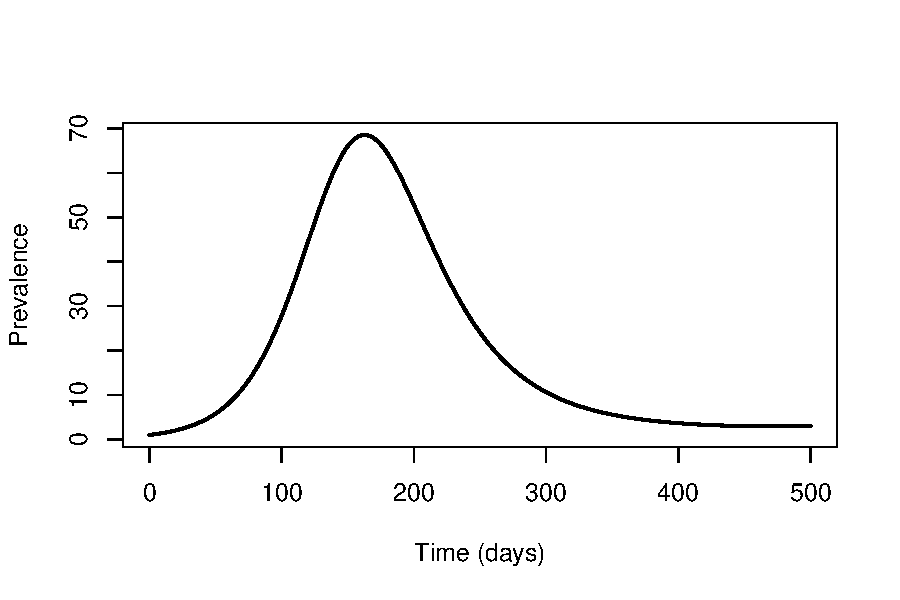
\includegraphics[width=\textwidth]{FIGS/course-01-SIRS_one_sim_prevalence-1.pdf}
  \end{center}
\end{frame}

\begin{frame}{I just did ...}

What I advise not to do: illustrate a mathematical result without adding anything to the result itself
\vfill
Let us make things a bit better. See the \href{https://raw.githubusercontent.com/julien-arino/3MC-2023-12-Arba-Minch/main/CODE/ODE_SIS_multiple_solutions.R}{code}
\end{frame}



\begin{frame}{}
  \begin{center}
    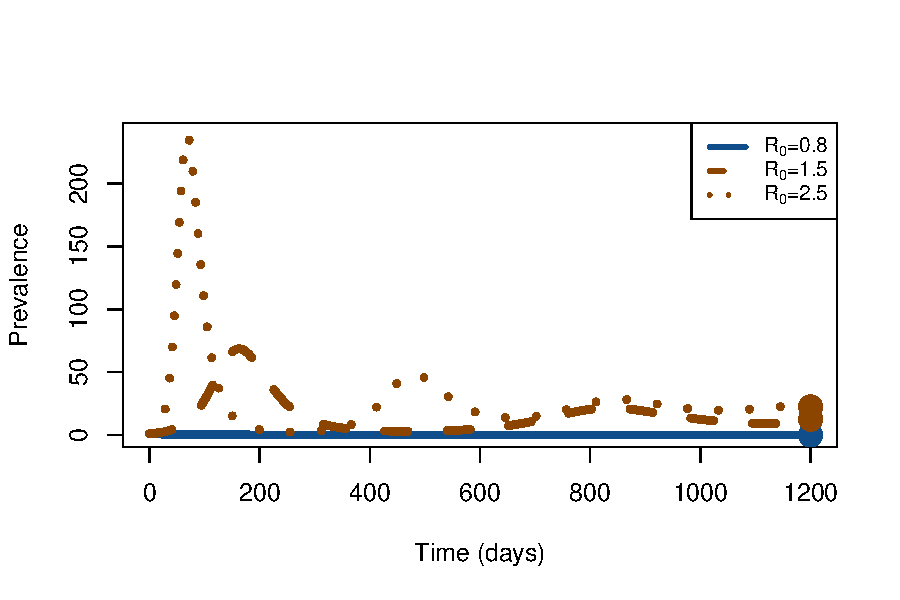
\includegraphics[width=\textwidth]{FIGS/course-01-SIRS_3_sims_prevalence-1.pdf}
  \end{center}
\end{frame}

\begin{frame}
We could continue, but with a model this simple, there is little  more to do: the 3 parameters of the system are combined within $\R_0$ and the latter summarises the dynamics well
\vfill
We are going to show something important: the bifurcation diagram
\vfill
We saw that when $\R_0<1$, $I\to 0$, whereas when $\R_0>1$, $I\to (1-1/\R_0)N$. Let us represent this (\href{https://raw.githubusercontent.com/julien-arino/3MC-2023-12-Arba-Minch/main/CODE/SIS_PEI_vs_R0.R}{code})
\end{frame}



\begin{frame}
  \begin{center}
    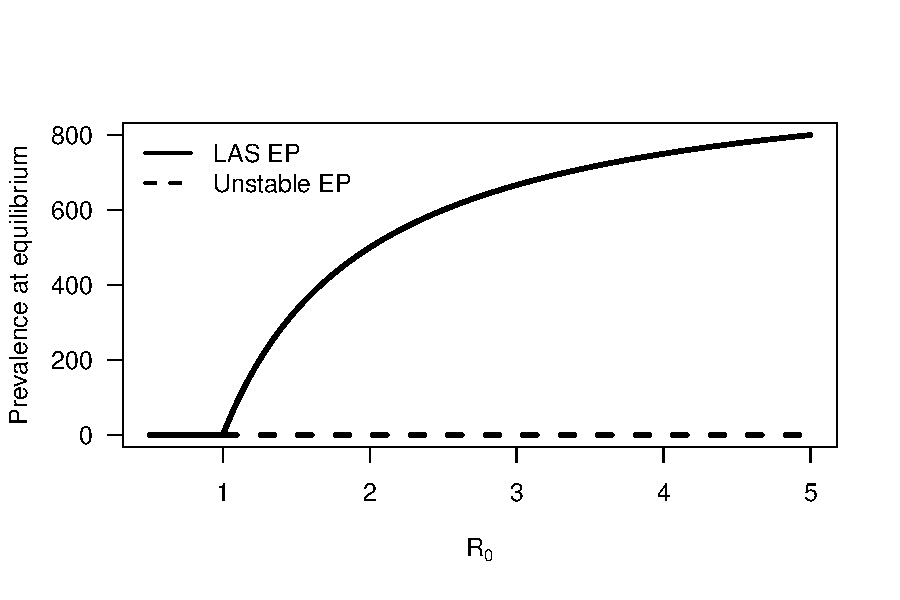
\includegraphics[width=\textwidth]{FIGS/course-01-SIRS_bifurcation_R0-1.pdf}
  \end{center}
\end{frame}



%%%%%%%%%%%%%%%%%%%%%%%%%%%
%%%%%%%%%%%%%%%%%%%%%%%%%%%
\subsection{Herd immunity in the SIRS model}
\newSubSectionSlide{FIGS-slides-admin/Gemini_Generated_Image_vqpscpvqpscpvqps.jpeg}

\begin{frame}{An SIRS model with vaccination}
Take SIRS model \eqref{sys:SIRS} and assume the following
\vfill
\begin{itemize}
\item Vaccination takes newborn individuals and moves them directly into the removed compartment, without them becoming infected/infectious
\vfill
\item A fraction $p$ is vaccinated at birth
\end{itemize}
\end{frame}

\begin{frame}{The model}
\begin{minipage}{0.25\textwidth}
  \def\skip{*-1.5}
  \begin{tikzpicture}[scale=1, transform shape]
    %% Regular nodes
    \node [circle, fill=green!50, text=black] at (0,0) (S) {$S$};
    \node [circle, fill=red!90, text=black] at (0,1\skip) (I) {$I$};
    \node [circle, fill=blue!90, text=black] at (0,2\skip) (R) {$R$};
    %% Fake nodes for arrows
    \node [above=1cm of S] (birthS) {};
    \node [below=1cm of R] (birthR) {};
    \node [left=0.5cm of S] (dS) {};
    \node [left=0.5cm of I] (dI) {};
    \node [left=0.5cm of R] (dR) {};
    %% Flows
    \path [line, very thick, red] (birthS) to node [midway, right] (TextNode) {$(1-p)b$} (S);
    \path [line, very thick, red] (birthR) to node [midway, right] (TextNode) {$pb$} (R);
    \path [line, very thick] (S) to node [midway, above] (TextNode) {$dS$} (dS);
    \path [line, very thick] (I) to node [midway, above] (TextNode) {$dI$} (dI);
    \path [line, very thick] (R) to node [midway, above] (TextNode) {$dR$} (dR);
    \path [line, very thick] (S) to node [midway, right] (TextNode) {$\beta SI$} (I);
    \path [line, very thick] (I) to node [midway, right] (TextNode) {$\gamma I$} (R);
    \draw [>=latex,->, thick, rounded corners] (R) -- (0.8,2\skip) -- (0.8,0) node[midway, right] {$\nu R$} -- (S);
    \end{tikzpicture}    
\end{minipage}
\begin{minipage}{0.7\textwidth}
  \begin{subequations} \label{sys:SIR_vacc}
  \begin{align}
    S\pprime &= (1-p)b+\nu R-dS-\beta SI \label{sys:SIR_vacc_dS} \\
    I\pprime &= \beta SI-(d+\gamma) I \label{sys:SIR_vacc_dI} \\
    R\pprime &= bp+\gamma I-(d+\nu)R \label{sys:SIR_vacc_dR}
  \end{align}    
  \end{subequations}
  \vskip1cm
  Consider the initial value problem consisting in \eqref{sys:SIR_vacc} to which we adjoin initial conditions $S(0)=S_0\geq 0$, $I(0)=I_0\geq 0$ and $R(0)=R_0\geq 0$
  \vskip1cm
  Typically, we assume $N_0=S_0+I_0+R_0>0$ to avoid a trivial case
  \end{minipage}
\end{frame}

\begin{frame}{This modification doesn't change much}
Equation \eqref{eq:total_pop_general} for the total population is unchanged
\vfill
The Jacobian \eqref{eq:SIRS_Jacobian} at arbitrary point is also unchanged
\vfill 
The DFE is affected, though; as a consequence, so is the reproduction number
\end{frame}

\begin{frame}{The DFE for the SIRS vaccination model}
Considering \eqref{sys:SIR_vacc} at equilibrium and substituting $I^\star=0$ into this system gives
\begin{align*}
0 &= (1-p)b+\nu R^\star-dS^\star \\
0 &= bp-(d+\nu)R^\star
\end{align*}
which we rewrite as the linear system
\[
\begin{pmatrix}
d & -\nu \\ 0 & d+\nu
\end{pmatrix}
\begin{pmatrix}
S^\star \\ R^\star
\end{pmatrix}
=
\begin{pmatrix}
(1-p)b \\ bp
\end{pmatrix}
\]
Thus
\begin{align*}
\begin{pmatrix}
S^\star \\ R^\star
\end{pmatrix}
&= \frac{1}{d(d+\nu)}
\begin{pmatrix}
d+\nu & \nu \\ 0 & d
\end{pmatrix}
\begin{pmatrix}
(1-p)b \\ pb
\end{pmatrix} \\
&= \frac{1}{d(d+\nu)}
\begin{pmatrix}
(d+\nu)(1-p)b+pb\nu \\ pbd
\end{pmatrix}
\end{align*}
\end{frame}

\begin{frame}
As a consequence, the DFE takes the form
\begin{equation}\label{eq:SIRS_vacc_DFE}
\bE_0^v := (S^\star,I^\star,R^\star) =
\left(
\left(1-p+\frac{p\nu}{d+\nu}\right)N^\star,0,
\frac{pd}{d+\nu}N^\star
\right)
\end{equation}
\vfill
Substituting \eqref{eq:SIRS_vacc_DFE} into the eigenvalue that determines stability of the DFE, $\beta S^\star-(d+\gamma)$, we get
\begin{align*}
\beta S^\star-(d+\gamma)<0 &\iff
\frac\beta{d+\gamma} S^\star <1 \\
&\iff 
\frac\beta{d+\gamma}
\left(1-p+\frac{p\nu}{d+\nu}\right)N^\star<1
\end{align*}
So we define
\begin{equation}\label{eq:SIRS_vacc_R0}
\R_0^v =
\frac\beta{d+\gamma}
\left(1-p+\frac{p\nu}{d+\nu}\right)N^\star
\end{equation}
\end{frame}


\begin{frame}{Herd immunity}
  Therefore 
  \begin{itemize}
  \item $\R_0^{\textrm{v}}<\R_0$ if $p>0$
  \item To control the disease, $\R_{\text{v}}$ must take a value less than 1, i.e.,
  \begin{equation}
    \R_{\text{v}}<1 \iff p> 1-\frac{1}{\R_0}
  \end{equation}
  \end{itemize}
  \vfill
  By vaccinating a fraction $p>1-1/\R_0$ of newborns, we thus are in a situation where the disease is eventually eradicated
  \vfill
  This is \defword{herd immunity} (\emph{bis repetita})
\end{frame}

%%%%%%%%%%%%%%
%%%%%%%%%%%%%%
\subsection{SLIRS model with constant population}
\newSubSectionSlide{FIGS-slides-admin/Gemini_Generated_Image_vqpscpvqpscpvqps.jpeg}

\frame{\frametitle{Incubation periods}
\begin{itemize}
\item SIS and SIR: progression from S to I is instantaneous
\vfill
\item Several incubation periods:
\end{itemize}
\begin{center}
\begin{tabular}{l|l}
Disease & Incubation period \\
\hline
Yersinia Pestis & 2-6 days \\
Ebola haemorrhagic fever (HF) & 2-21 days \\
Marburg HF & 5-10 days \\
Lassa fever & 1-3 weeks \\
Tse-tse & weeks--months \\
HIV/AIDS & months--years
\end{tabular}
\end{center}
}

\frame{\frametitle{Hypotheses}
\begin{itemize}
\item There is demography
\item New individuals are born at a constant rate $b$
\item
There is no vertical transmssion: all ``newborns'' are susceptible
\item The disease is non lethal, it causes no additional mortality
\item New infections occur at the rate $f(S,I,N)$
\item There is a period of incubation for the disease
\item There is a period of time after recovery during which the disease confers immunity to reinfection (immune period)
\end{itemize} 
}

\frame{\frametitle{SLIRS}
\begin{minipage}{0.2\textwidth}
  \def\skip{*-1.5}
  \begin{tikzpicture}[scale=1, transform shape]
    %% Regular nodes
    \node [circle, fill=green!50, text=black] at (0,0) (S) {$S$};
    \node [circle, fill=red!50, text=black] at (0,1\skip) (L) {$L$};
    \node [circle, fill=red!90, text=black] at (0,2\skip) (I) {$I$};
    \node [circle, fill=blue!50, text=black] at (0,3\skip) (R) {$R$};
    %% Fake nodes for arrows
    \node [above=0.75cm of S] (birth) {};
    \node [left=0.5cm of S] (dS) {};
    \node [left=0.5cm of L] (dL) {};
    \node [left=0.5cm of I] (dI) {};
    \node [left=0.5cm of R] (dR) {};
    %% Flows (demography)
    \path [line, very thick] (birth) to node [midway, left] (TextNode) {$b$} (S);
    \path [line, very thick] (S) to node [midway, above] (TextNode) {$dS$} (dS);
    \path [line, very thick] (L) to node [midway, below] (TextNode) {$dL$} (dL);
    \path [line, very thick] (I) to node [midway, below] (TextNode) {$dI$} (dI);
    \path [line, very thick] (R) to node [midway, below] (TextNode) {$dR$} (dR);
    %% Flows (demography)
    \path [line, very thick] (S) to node [midway, left] (TextNode) {$f(S,I,N)$} (L);
    \path [line, very thick] (L) to node [midway, left] (TextNode) {$\varepsilon L$} (I);
    \path [line, very thick] (I) to node [midway, left] (TextNode) {$\gamma I$} (R);
    \draw [>=latex,->, thick, rounded corners] (R) -- (0.75,3\skip) -- (0.75,0) node[midway,above,sloped] {$\nu R$} -- (S);
  \end{tikzpicture}    
\end{minipage}
\quad
\begin{minipage}{0.7\textwidth}
The model is as follows:
\begin{subequations}\label{sys:SLIRS}
\begin{align}
S\pprime &= b+\nu R-dS-f(S,I,N) \label{sys:SLIRS_dS} \\
L\pprime &= f(S,I,N) -(d+\varepsilon)L \label{sys:SLIRS_dL} \\
I\pprime &= \varepsilon L -(d+\gamma)I \label{sys:SLIRS_dI} \\
R\pprime &= \gamma I-(d+\nu)R \label{sys:SLIRS_dR} 
\end{align}
\end{subequations}
\vfill
Meaning of the parameters:
\begin{itemize}
\item $1/\varepsilon$ average duration of the incubation period
\item $1/\gamma$ average duration of infectious period
\item $1/\nu$ average duration of immune period
\end{itemize}
\end{minipage}
}



%%%%%%%%%%%%%%%%%%%%%%%
%%%%%%%%%%%%%%%%%%%%%%%
\subsection{Computing $\R_0$ more efficiently}
\newSubSectionSlide{FIGS-slides-admin/Gemini_Generated_Image_vqpscpvqpscpvqps.jpeg}

\maxFrameImage{FIGS/PvdDWatmough2002.png}


\frame{\frametitle{The basic reproduction number $\R_0$}
Used frequently in epidemiology (not only math epi)
\begin{definition}[$R_0$]
The basic reproduction number $\R_0$ is the average number of secondary cases generated by the introduction of an infectious individual in a wholly susceptible population
\end{definition}
\begin{itemize}
\item If $\R_0<1$, then on average, each infectious individual infects less than one other person, so the epidemic has chances of dying out
\item If $\R_0>1$, then on average, each infectious individual infects more than one other person and the disease can become established in the population (or there will be a major epidemic)
\end{itemize}
}

\frame{\frametitle{Computation of $\R_0$}
Mathematically, $\R_0$ is a bifurcation parameter aggregating some of the model parameters and such that the disease free equilibrium (DFE) loses its local asymptotic stability when $\R_0=1$ is crossed from left to right
\vfill
\begin{itemize}
\item
As a consequence, $\R_0$ is found by considering the spectrum of the Jacobian matrix of the system evaluated at the DFE
\vfill
\item
The matrix quickly becomes hard to deal with (size and absence of ``pattern'') and the form obtained is not unique, which is annoying when trying to interpret $\R_0$
\end{itemize}
}

\begin{frame}{Preliminary setup of PvdD \& Watmough 2002}
$x=(x_1,\ldots,x_n)^T$, $x_i\geq 0$, with the first $m<n$ compartments the infected ones
\vfill
$X_s$ the set of all disease free states: 
\[
X_s=\{x\geq 0| x_i=0, i=1,\ldots,m\}
\]
\vfill
Distinguish new infections from all other changes in population
\begin{itemize}
\item $F_i(x)$ rate of appearance of new infections in compartment $i$
\item $V_i^+(x)$ rate of transfer of individuals into compartment $i$ by all other means
\item $V_i^-(x)$ rate of transfer of individuals out of compartment $i$
\end{itemize}
\vfill
Assume each function continuously differentiable at least twice in each variable
\vfill
\[
x_i' = f_i(x)=F_i(x)-V_i(x),\quad i=1,\ldots,n
\]
where $V_i=V_i^--V_i^+$
\end{frame}

\begin{frame}{Some assumptions}
\bbullet\textbf{(A1)}
If $x\geq 0$, then $F_i,V_i^+,V_i^-\geq 0$ for $i=1,\ldots,n$
\vfill
Since each function represents a directed transfer of individuals, all are non-negative
\vfill
\bbullet\textbf{(A2)} 
If $x_i=0$ then $V_i^-=0$. In particular, if $x\in X_s$, then $V_i^-=0$ for $i=1,\ldots,m$
\vfill
If a compartment is empty, there can be no transfer of individuals out of the compartment by death, infection, nor any other means
\end{frame}

\begin{frame}
\bbullet \textbf{(A3)} $F_i=0$ if $i>m$
\vfill
The incidence of infection for uninfected compartments is zero
\vfill
\bbullet \textbf{A4} If $x\in X_s$ then $F_i(x)=0$ and $V_i^+(x)=0$ for $i=1,\ldots,m$
\vfill
Assume that if the population is free of disease then the population will remain free of disease; i.e., there is no (density independent) immigration of infectives
\end{frame}

\begin{frame}{One last assumption for the road}
Let $x_0$ be a DFE of the system, i.e., a (locally asymptotically) stable equilibrium solution of the disease free model, i.e., the system restricted to $X_s$. We need not assume that the model has a unique DFE
\vfill
Let $Df(x_0)$ be the Jacobian matrix $[\partial f_i/\partial x_j]$. Some derivatives are one sided, since $x_0$ is on the domain boundary
\vfill
\textbf{(A5)} If $F(x)$ is set to zero, then all eigenvalues of $Df(x_0)$ have negative real parts
\vfill
Note: if the method ever fails to work, it is usually with (A5) that lies the problem
\end{frame}

\begin{frame}{Stability of the DFE as function of $\mathcal{R}_0$}
\begin{theorem}\label{th:R0_VdDW}
Suppose the DFE exists. Let then
\[
\mathcal{R}_0=\rho(FV^{-1})
\]
with matrices $F$ and $V$ obtained as indicated. Assume conditions (A1) through (A5) hold. Then
\begin{itemize}
\item if $\mathcal{R}_0<1$, then the DFE is LAS
\item if $\mathcal{R}_0>1$, the DFE is unstable
\end{itemize}
\end{theorem}
\vfill
Important to stress \emph{local} nature of stability that is deduced from this result. We will see later that even when $\mathcal{R}_0<1$, there can be several positive equilibria
\end{frame}

\begin{frame}{Direction of the bifurcation at $\mathcal{R}_0=1$}
$\mu$ bifurcation parameter s.t. $\mathcal{R}_0<1$ for $\mu<0$ and $\mathcal{R}_0>1$ for $\mu>0$ and $x_0$ DFE for all values of $\mu$ and consider the system
\begin{equation}
\label{eq:sys_PvdDW}
x'=f(x,\mu)
\end{equation}
\vfill
Write 
\[
D_xf(x_0,0)=
\left. 
  D(\mathcal{F}(x_0)-\mathcal{V}(x_0))
\right|_{\mathcal{R}_0=1}
\]
as block matrix
\[
D\mathcal{F}(x_0)
=\begin{pmatrix}
F & 0 \\ 0 & 0
\end{pmatrix},
\quad
D\mathcal{V}(x_0)
=\begin{pmatrix}
V & 0 \\ J_3 & J_4
\end{pmatrix}
\]
\end{frame}

\begin{frame}
Write $[\alpha_{\ell k}]$, $\ell=m+1,\ldots,n$, $k=1,\ldots,m$ the $(\ell-m,k)$ entry of $-J_4^{-1}J_3$ and let $v$ and $w$ be left and right eigenvectors of $D_xf(x_0,0)$ s.t. $vw=1$
\vfill
Let
\begin{equation}
\label{eq:PvdDW_a}
a =\sum_{i,j,k=1}^m
v_iw_jw_k
\left(
\frac 12 
\frac{\partial^2f_i}{\partial x_j\partial x_k}(x_0,0)
+\sum_{\ell=m+1}^n
\alpha_{\ell k}
\frac{\partial^2f_i}{\partial x_j\partial x_\ell}(x_0,0)
\right)
\end{equation}
\vfill
\begin{equation}
\label{eq:PvdDW_b}
b
=vD_{x\mu}f(x_0,0)w
=\sum_{i,j=1}^n v_iw_j
\frac{\partial^2f_i}{\partial x_j\partial\mu}
(x_0,0)
\end{equation}
\end{frame}

\begin{frame}
\begin{theorem}
Consider model $\eqref{eq:sys_PvdDW}$ with $f(x,\mu)$ satisfying conditions (A1)–(A5) and $\mu$ as described above
\vskip1cm
Assume that the zero eigenvalue of $D_xf(x_0,0)$ is simple
\vskip1cm
Define $a$ and $b$ by $\eqref{eq:PvdDW_a}$ and $\eqref{eq:PvdDW_b}$; assume that $b\neq 0$. Then $\exists\delta > 0$ s.t.
\begin{itemize}
\item if $a < 0$, then there are LAS endemic equilibria near $x_0$ for $0 < \mu < \delta$
\item if $a > 0$, then there are unstable endemic equilibria near $x_0$ for $-\delta < \mu < 0$
\end{itemize}
\end{theorem}
\end{frame}


\frame{\frametitle{Example of the SLIRS model \eqref{sys:SLIRS}}
Variation of the infected variables in \eqref{sys:SLIRS} are described by
\begin{align*}
L\pprime &= f(S,I,N)-(\varepsilon+d) L \\
I\pprime &= \varepsilon L -(d+\gamma) I
\end{align*}
Write
\begin{equation}
\I\pprime = 
\left(
\begin{matrix}
L \\
I
\end{matrix}
\right)'
=\left(
\begin{matrix}
f(S,I,N) \\
0
\end{matrix}
\right)
-
\left(
\begin{matrix}
(\varepsilon+d) L \\
(d+\gamma) I-\varepsilon L
\end{matrix}
\right)=:\mathcal{F}-\mathcal{V}
\end{equation}
}


\frame{
Denote
\[
f_L^{\,\star}:=
\left.\frac{\partial}{\partial L}f
\right|_{(S,I,R)=\bE_0}
\quad\quad 
f_I^{\,\star}:=
\left.\frac{\partial}{\partial I}f
\right|_{(S,I,R)=\bE_0}
\]
the values of the partials of the incidence function at the DFE $\bE_0$
\vfill
Compute the Jacobian matrices of vectors $\F$ and $\V$ at the DFE $\bE_0$
\begin{equation}
F=\left(
\begin{matrix}
f_L^{\,\star} & f_I^{\,\star} \\
0 & 0
\end{matrix}
\right)
\quad\text{and}\quad
V=\left(
\begin{matrix}
\varepsilon+d & 0 \\
-\varepsilon & d+\gamma
\end{matrix}
\right)
\end{equation}
}

\frame{
Thus
\[
V^{-1}=\frac{1}{(d+\varepsilon)(d+\gamma)}
\left(
\begin{matrix}
d+\gamma & 0 \\
\varepsilon & d+\varepsilon
\end{matrix}
\right)
\]
\vfill
Also, in the case $N$ is constant, $\partial f/\partial L=0$ and thus
\[
FV^{-1}=\frac{f_I^{\,\star}}
{(d+\varepsilon)(d+\gamma)}
\left(
\begin{matrix}
\varepsilon 
& d+\varepsilon  \\
0 & 0
\end{matrix}
\right)
\]
\vfill
As a consequence,
\[
\R_0=\varepsilon
\frac{f_I^{\,\star}}
{(d+\varepsilon)(d+\gamma)}
\]
}


\frame{
\begin{theorem}\label{th:R0_SEIRS}
Let
\begin{equation}\label{eq:R0_SEIRS}
\R_0=
\frac{\varepsilon f_I^{\,\star}}
{(d+\varepsilon)(d+\gamma)}
\end{equation}
Then
\begin{itemize}
\item if $\R_0<1$, the DFE is LAS
\item if $\R_0>1$, the DFE is unstable
\end{itemize}
\end{theorem}
\vfill
It is important here to stress that the result we obtain concerns the \textbf{local} asymptotic stability. We see later that even when $\R_0<1$, there can be several locally asymptotically stable equilibria
}


\frame{\frametitle{Application}
The DFE is
\[
(\bar S,\bar L,\bar I,\bar R)=(N,0,0,0)
\]
\begin{itemize}
\item Mass action incidence (frequency-dependent contacts):
 \[
f_I^{\,\star}=\beta\bar S \Rightarrow\R_0 =
\frac{\epsilon\beta N}{(\epsilon+d)(\gamma+d)} 
\]
\item Standard incidence (proportion-dependent contacts):
\[
f_I^{\,\star}=\frac{\beta\bar S}{N}
\Rightarrow\R_0 = \frac{\epsilon\beta}{(\epsilon+d)(\gamma+d)}
\]
\end{itemize}
}


\frame{\frametitle{Links between SLIRS-type models}
{ %\footnotesize
\begin{align*}
S\pprime&=b+\nu R-dS-f(S,I,N) \\
L\pprime&=f(S,I,N)-(d+\varepsilon) L \\
I\pprime&=\varepsilon L-(d+\gamma)I \\
R\pprime&=\gamma I-(d+\nu)R
\end{align*}}
\begin{center}
\begin{tabular}{c|l}
\hline
SLIR & SLIRS where $\nu=0$ \\
SLIS & Limit of SLIRS when $\nu\to\infty$ \\
SLI & SLIR where $\gamma=0$ \\
SIRS & Limit of SLIRS when $\varepsilon\to\infty$ \\
SIR & SIRS where $\nu=0$ \\
SIS & Limit of SIRS when $\nu\to\infty$ \\
& Limit SLIS when $\varepsilon\to\infty$ \\
SI & SIS where $\nu=0$ 
\end{tabular}
\end{center}
}

\frame{\frametitle{Values of $\R_0$}
$(\bar S,\bar I,\bar N)$ values of $S,I$ and $N$ at DFE. Denote $\bar f_I=\partial f/\partial I(\bar S,\bar I,\bar N)$.
\begin{center}
\begin{tabular}{c|c}
\hline
SLIRS & 
$\frac{\varepsilon\bar f_I}{(d+\varepsilon)(d+\gamma)}$ \\
SLIR & 
$\frac{\varepsilon\bar f_I}{(d+\varepsilon)(d+\gamma)}$ \\
SLIS & 
$\frac{\varepsilon\bar f_I}{(d+\varepsilon)(d+\gamma)}$ \\
SLI & 
$\frac{\varepsilon\bar f_I}{(d+\varepsilon)(d+\gamma)}$ \\
& \\
SIRS & 
$\frac{\varepsilon\bar f_I}{d+\gamma}$ \\
SIR & $\frac{\bar f_I}{d+\gamma}$ \\
SIS & $\frac{\bar f_I}{d+\gamma}$ \\
SI & $ \frac{\bar f_I}{d+\gamma}$ 
\end{tabular}
\end{center}
}


%%%%%%%%%%%%%%%%%%%%%%%
%%%%%%%%%%%%%%%%%%%%%%%
\subsection{A better vaccination model?}
\newSubSectionSlide{FIGS-slides-admin/Gemini_Generated_Image_vqpscpvqpscpvqps.jpeg}

\maxFrameImage{FIGS/ArinoMccluskeyPvdD.png}

\begin{frame}{SLIRS with vaccination}
\centering
  \def\skip{*2.5}
  \begin{tikzpicture}[scale=1.5, transform shape]
    %% Regular nodes
    \node [circle, fill=green!50, text=black] at (0,0) (S) {$S$};
    \node [circle, fill=red!90, text=black] at (1\skip,0) (I) {$I$};
    \node [circle, fill=blue!50, text=black] at (2\skip,0) (R) {$R$};
    \node [circle, fill=red!50, text=black] at (0.5\skip,-1\skip) (V) {$V$};
    %% Fake nodes for arrows
    \node [left=0.75cm of S] (birth) {};
    \node [below=0.5cm of S] (dS) {};
    \node [below=0.5cm of I] (dI) {};
    \node [below=0.5cm of R] (dR) {};
    \node [below=0.5cm of V] (dV) {};
    %% Flows (demography)
    \path [line, very thick] (birth) to node [midway, above] (TextNode) {$b$} (S);
    \path [line, very thick] (S) to node [midway, left] (TextNode) {$dS$} (dS);
    \path [line, very thick] (I) to node [midway, right] (TextNode) {$dI$} (dI);
    \path [line, very thick] (R) to node [midway, left] (TextNode) {$dR$} (dR);
    \path [line, very thick] (V) to node [midway, left] (TextNode) {$dV$} (dV);
    %% Flows
    \path [line, very thick] (S) to node [midway, above] (TextNode) {$\beta SI/N$} (I);
    \path [line, very thick, bend left=10] (S) to node [near start, right] (TextNode) {$\phi S$} (V);
    \path [line, very thick, bend left=10] (V) to node [near start, left] (TextNode) {$\varphi V$} (S);
    \path [line, very thick] (V) to node [midway, above, sloped] (TextNode) {$\sigma\beta SI/N$} (I);
    \path [line, very thick] (I) to node [midway, above] (TextNode) {$\gamma I$} (R);
    \draw [>=latex,->, thick, rounded corners] (R) -- (2\skip,0.75) -- (0,0.75) node[midway,above,sloped] {$\nu R$} -- (S);
  \end{tikzpicture}    
\end{frame}

\begin{frame}{The usual situation}
\centering
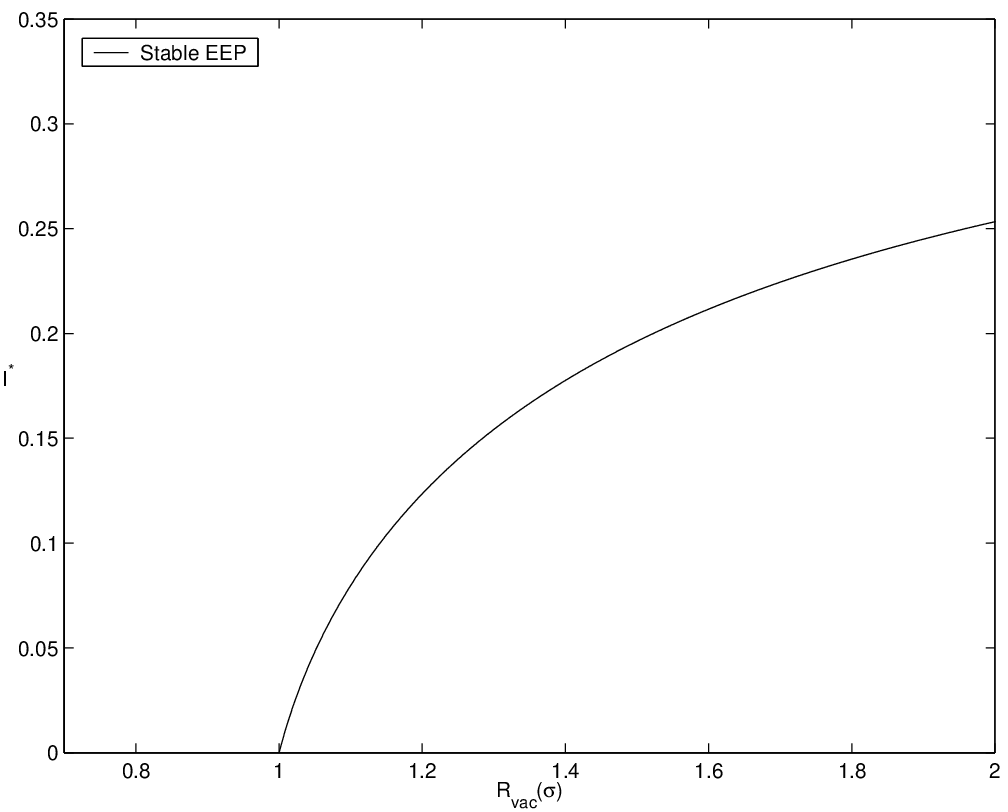
\includegraphics[width=0.7\textwidth]{FIGS/SIRV_bif_forward}
\end{frame}

\begin{frame}{What can happen with vaccination -- Backward bifurcation}
\centering
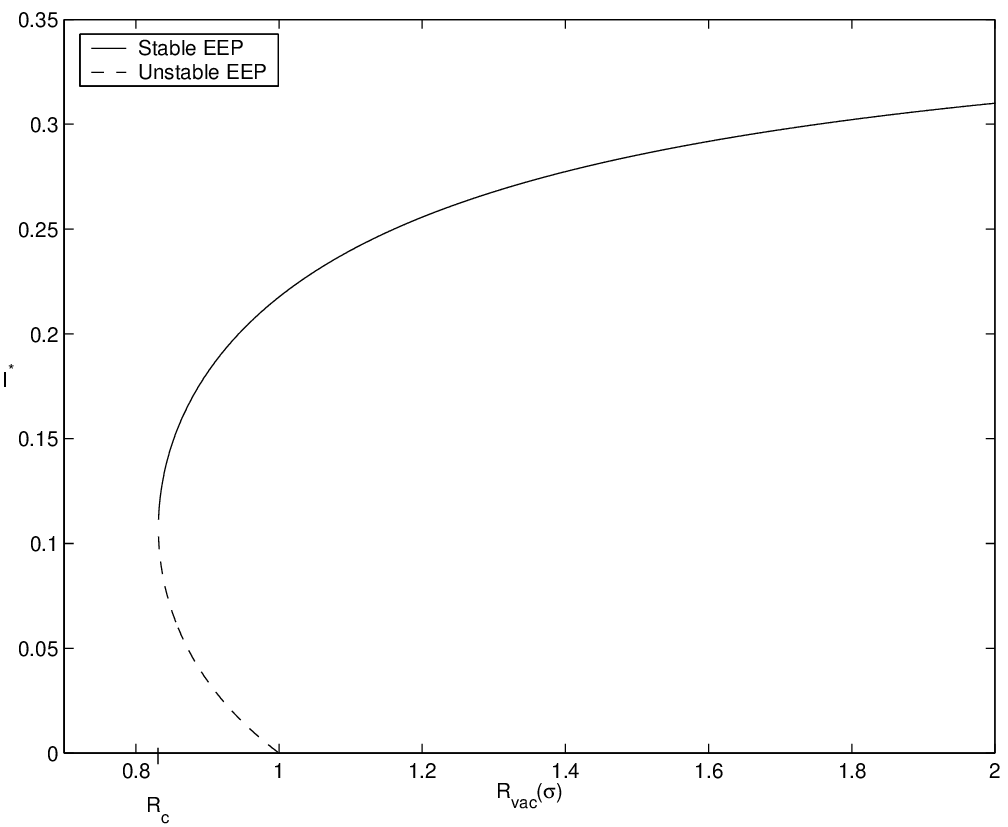
\includegraphics[width=0.7\textwidth]{FIGS/SIRV_bif_backward}
\end{frame}


%%%%%%%%%%%%%%%%%%%%
%%%%%%%%%%%%%%%%%%%%
%%%%%%%%%%%%%%%%%%%%
%%%%%%%%%%%%%%%%%%%%
\section{What if there's another guest at the party?}
\newSectionSlide{FIGS-slides-admin/Gemini_Generated_Image_4ls25f4ls25f4ls2.jpeg}

%%%%%%%%%%%%%%%%%%%%
%%%%%%%%%%%%%%%%%%%%
\subsection{Two Ross-Macdonald-type models}
\newSubSectionSlide{FIGS-slides-admin/Gemini_Generated_Image_4ls25f4ls25f4ls2.jpeg}
\begin{frame}
See, e.g., Simoy \& Aparicio, \href{https://doi.org/10.1016/j.actatropica.2020.105452}{Ross-Macdonald models: Which one should we use?}, \emph{Acta Tropica} (2020)
\vfill
Ross introduced the model in 1911. Later ``tweaked'' by Macdonald to include mosquito latency period
\vfill
Here, I show a version in the paper cited, with some notation changed
\end{frame}

\begin{frame}
\centering
\resizebox{\textwidth}{!}{
  \def\horskip{*2}
  \def\verskip{*2}
  \begin{tikzpicture}[%transform canvas={scale=1.3},
      auto,
      cloud/.style={minimum width={width("N-1")+2pt},
      draw, 
      ellipse,
      fill=gray!20}]
    %% Hosts
    \node [cloud, fill=green!50] at (0,0) (SH) {$S_H$};
    \node [cloud, fill=red!50] at (1\horskip,0) (IH) {$I_H$};
    \node [cloud, fill=blue!50] at (2\horskip,0) (RH) {$R_H$};
    %% Vectors
    \node [cloud, fill=green!50] at (0,-1\verskip) (SV) {$S_V$};
    \node [cloud, fill=red!50] at (1\horskip,-1\verskip) (IV) {$I_V$};
    %% Births
    \node [left=0.75cm of SH] (birthH) {};
    \node [left=0.75cm of SV] (birthV) {};
    %% Deaths
    \node [below=0.25\verskip of SH] (dSH) {};
    \node [below=0.25\verskip of IH] (dIH) {};
    \node [below=0.25\verskip of RH] (dRH) {};
    \node [below=0.25\verskip of SV] (dSV) {};
    \node [below=0.25\verskip of IV] (dIV) {};
    %%
    \path [line, very thick] (SH) to node [midway,above,sloped] (TextNode) {$\beta_HI_V\frac{S_H}{H}$} (IH);
    \path [line, very thick] (IH) to node [midway,above,sloped] (TextNode) {$\gamma_H I_H$} (RH);
    \path [line, very thick] (SV) to node [midway,below,sloped] (TextNode) {$\beta_VS_V\frac{I_H}{H}$} (IV);
    \path [line, dotted, very thick] (IV) to node [midway,below,sloped] (TextNode) {} (SH);
    \path [line, dotted, very thick] (IH) to node [midway,above,sloped] (TextNode) {} (SV);
    %% Demography
    \path [line, very thick] (birthH) to node [midway,above] (TextNode) {$b_H$} (SH);
    \path [line, very thick] (birthV) to node [midway,above] (TextNode) {$b_V$} (SV);
    \path [line, very thick] (SH) to node [near end,left] (TextNode) {$d_HS_H$} (dSH);
    \path [line, very thick] (IH) to node [near end,right] (TextNode) {$d_HI_H$} (dIH);
    \path [line, very thick] (RH) to node [near end,right] (TextNode) {$d_HR_H$} (dRH);
    \path [line, very thick] (SV) to node [near end,left] (TextNode) {$d_VS_V$} (dSV);
    \path [line, very thick] (IV) to node [near end,right] (TextNode) {$d_VI_V$} (dIV);
  \end{tikzpicture}
}
\end{frame}

\begin{frame}{Reproduction number}
\begin{equation}\label{eq:vector_host_1}
\R_0 =
\frac{\beta_H\beta_V}{(\gamma_H+\gamma_V)d_V}\
\frac{V^\star}{H^\star}
\end{equation}
where $H^\star$ and $V^\star$ are the total host and vector populations, respectively
\end{frame}


\begin{frame}
\centering
\resizebox{\textwidth}{!}{
  \def\horskip{*2}
  \def\verskip{*2}
  \begin{tikzpicture}[%transform canvas={scale=1.3},
      auto,
      cloud/.style={minimum width={width("N-1")+2pt},
      draw, 
      ellipse,
      fill=gray!20}]
    %% Hosts
    \node [cloud, fill=green!50] at (0,0) (SH) {$S_H$};
    \node [cloud, fill=red!10] at (1\horskip,0) (LH) {$L_H$};
    \node [cloud, fill=red!50] at (2\horskip,0) (IH) {$I_H$};
    \node [cloud, fill=blue!50] at (3\horskip,0) (RH) {$R_H$};
    %% Vectors
    \node [cloud, fill=green!50] at (0,-1\verskip) (SV) {$S_V$};
    \node [cloud, fill=red!10] at (1\horskip,-1\verskip) (LV) {$L_V$};
    \node [cloud, fill=red!50] at (2\horskip,-1\verskip) (IV) {$I_V$};
    %% Births
    \node [left=0.75cm of SH] (birthH) {};
    \node [left=0.75cm of SV] (birthV) {};
    %% Deaths
    \node [above=0.5\verskip of SH] (dSH) {};
    \node [above=0.5\verskip of LH] (dLH) {};
    \node [above=0.5\verskip of IH] (dIH) {};
    \node [above=0.5\verskip of RH] (dRH) {};
    \node [below=0.5\verskip of SV] (dSV) {};
    \node [below=0.5\verskip of LV] (dLV) {};
    \node [below=0.5\verskip of IV] (dIV) {};
    %%
    \path [line, very thick] (SH) to node [midway,above,sloped] (TextNode) {$\beta_HI_V\frac{S_H}{H}$} (LH);
    \path [line, very thick] (LH) to node [midway,above,sloped] (TextNode) {$\varepsilon_H L_H$} (IH);
    \path [line, very thick] (IH) to node [midway,above,sloped] (TextNode) {$\gamma_H I_H$} (RH);
    \path [line, very thick] (SV) to node [midway,below,sloped] (TextNode) {$\beta_VS_V\frac{I_H}{H}$} (LV);
    \path [line, very thick] (LV) to node [midway,below,sloped] (TextNode) {$\varepsilon_V L_V$} (IV);
    \path [line, dotted, very thick] (IV) to node [midway,below,sloped] (TextNode) {} (SH);
    \path [line, dotted, very thick] (IH) to node [midway,above,sloped] (TextNode) {} (SV);
    %% Demography
    \path [line, very thick] (birthH) to node [midway,above] (TextNode) {$b_H$} (SH);
    \path [line, very thick] (birthV) to node [midway,above] (TextNode) {$b_V$} (SV);
    \path [line, very thick] (SH) to node [near end,right] (TextNode) {$d_HS_H$} (dSH);
    \path [line, very thick] (LH) to node [near end,right] (TextNode) {$d_HL_H$} (dLH);
    \path [line, very thick] (IH) to node [near end,right] (TextNode) {$d_HI_H$} (dIH);
    \path [line, very thick] (RH) to node [near end,right] (TextNode) {$d_HR_H$} (dRH);
    \path [line, very thick] (SV) to node [near end,right] (TextNode) {$d_VS_V$} (dSV);
    \path [line, very thick] (LV) to node [near end,right] (TextNode) {$d_VL_V$} (dLV);
    \path [line, very thick] (IV) to node [near end,right] (TextNode) {$d_VI_V$} (dIV);
  \end{tikzpicture}
}
\end{frame}

\begin{frame}{Reproduction number}
\begin{equation}\label{eq:vector_host_2}
\R_0 =
\frac{\beta_H\beta_V}{(\gamma_H+\gamma_V)d_V}\
\frac{\varepsilon_V}{d_V+\varepsilon_V}\
\frac{\varepsilon_H}{d_H+\varepsilon_H}\
\frac{V^\star}{H^\star}
\end{equation}
where $H^\star$ and $V^\star$ are the total host and vector populations, respectively
\vfill
Here
\[
f_X = \frac{\varepsilon_X}{d_X+\varepsilon_X}
\]
are the fractions of latent individuals (of type $X=\{V,H\}$) who survive the latency period
\end{frame}


%%%%%%%%%%%%%%%%%%%%
%%%%%%%%%%%%%%%%%%%%
\subsection{A little complexification of Ross-Macdonald}
\newSubSectionSlide{FIGS-slides-admin/Gemini_Generated_Image_mco1ecmco1ecmco1.jpeg}

\begin{frame}{Recall this guy?}
\centering
\resizebox{\textwidth}{!}{
  \def\horskip{*2}
  \def\verskip{*2}
  \begin{tikzpicture}[%transform canvas={scale=1.3},
      auto,
      cloud/.style={minimum width={width("N-1")+2pt},
      draw, 
      ellipse,
      fill=gray!20}]
    %% Hosts
    \node [cloud, fill=green!50] at (0,0) (SH) {$S_H$};
    \node [cloud, fill=red!50] at (1\horskip,0) (IH) {$I_H$};
    \node [cloud, fill=blue!50] at (2\horskip,0) (RH) {$R_H$};
    %% Vectors
    \node [cloud, fill=green!50] at (0,-1\verskip) (SV) {$S_V$};
    \node [cloud, fill=red!50] at (1\horskip,-1\verskip) (IV) {$I_V$};
    %% Births
    \node [left=0.75cm of SH] (birthH) {};
    \node [left=0.75cm of SV] (birthV) {};
    %% Deaths
    \node [below=0.25\verskip of SH] (dSH) {};
    \node [below=0.25\verskip of IH] (dIH) {};
    \node [below=0.25\verskip of RH] (dRH) {};
    \node [below=0.25\verskip of SV] (dSV) {};
    \node [below=0.25\verskip of IV] (dIV) {};
    %%
    \path [line, very thick] (SH) to node [midway,above,sloped] (TextNode) {$\beta_HI_V\frac{S_H}{H}$} (IH);
    \path [line, very thick] (IH) to node [midway,above,sloped] (TextNode) {$\gamma_H I_H$} (RH);
    \path [line, very thick] (SV) to node [midway,below,sloped] (TextNode) {$\beta_VS_V\frac{I_H}{H}$} (IV);
    \path [line, dotted, very thick] (IV) to node [midway,below,sloped] (TextNode) {} (SH);
    \path [line, dotted, very thick] (IH) to node [midway,above,sloped] (TextNode) {} (SV);
    %% Demography
    \path [line, very thick] (birthH) to node [midway,above] (TextNode) {$b_H$} (SH);
    \path [line, very thick] (birthV) to node [midway,above] (TextNode) {$b_V$} (SV);
    \path [line, very thick] (SH) to node [near end,left] (TextNode) {$d_HS_H$} (dSH);
    \path [line, very thick] (IH) to node [near end,right] (TextNode) {$d_HI_H$} (dIH);
    \path [line, very thick] (RH) to node [near end,right] (TextNode) {$d_HR_H$} (dRH);
    \path [line, very thick] (SV) to node [near end,left] (TextNode) {$d_VS_V$} (dSV);
    \path [line, very thick] (IV) to node [near end,right] (TextNode) {$d_VI_V$} (dIV);
  \end{tikzpicture}
}
\end{frame}


\begin{frame}{Let us add a few arrows}
\centering
\resizebox{0.8\textwidth}{!}{
  \def\horskip{*2}
  \def\verskip{*2}
  \begin{tikzpicture}[%transform canvas={scale=1.3},
      auto,
      cloud/.style={minimum width={width("N-1")+2pt},
      draw, 
      ellipse,
      fill=gray!20}]
    %% Hosts
    \node [cloud, fill=green!50] at (0,0) (SH) {$S_H$};
    \node [cloud, fill=red!50] at (1\horskip,0) (IH) {$I_H$};
    \node [cloud, fill=blue!50] at (2\horskip,0) (RH) {$R_H$};
    %% Vectors
    \node [cloud, fill=green!50] at (0,-1\verskip) (SV) {$S_V$};
    \node [cloud, fill=red!50] at (1\horskip,-1\verskip) (IV) {$I_V$};
    %% Births
    \node [left=0.75cm of SH] (birthH) {};
    \node [left=0.75cm of SV] (birthV) {};
    %% Deaths
    \node [below=0.25\verskip of SH] (dSH) {};
    \node [below=0.25\verskip of IH] (dIH) {};
    \node [below=0.25\verskip of RH] (dRH) {};
    \node [below=0.25\verskip of SV] (dSV) {};
    \node [below=0.25\verskip of IV] (dIV) {};
    %%
    \path [line, very thick] (SH) to node [midway,above,sloped] (TextNode) {$\Phi_H$} (IH);
    \path [line, very thick] (IH) to node [midway,above,sloped] (TextNode) {$\gamma_H I_H$} (RH);
    \path [line, very thick] (SV) to node [midway,below,sloped] (TextNode) {$\Phi_V$} (IV);
    \path [line, dotted, very thick] (IV) to node [midway,below,sloped] (TextNode) {} (SH);
    \path [line, dotted, very thick] (IH) to node [midway,above,sloped] (TextNode) {} (SV);
    \draw [>=latex,->, thick, rounded corners] (IH) -- (1\horskip,0.75) -- (0,0.75) node[midway,above,sloped] {$\rho_H I_H$} -- (SH);
    \draw [>=latex,->, thick, rounded corners] (RH) -- (2\horskip,1.5) -- (-0.35,1.5) node[midway,above,sloped] {$\nu_H R_H$} -- (SH.north west);
    %% Demography
    \path [line, very thick] (birthH) to node [midway,above] (TextNode) {$b_H$} (SH);
    \path [line, very thick] (birthV) to node [midway,above] (TextNode) {$b_V$} (SV);
    \path [line, very thick] (SH) to node [near end,left] (TextNode) {$d_HS_H$} (dSH);
    \path [line, very thick] (IH) to node [near end,right] (TextNode) {$d_HI_H$} (dIH);
    \path [line, very thick] (RH) to node [near end,right] (TextNode) {$d_HR_H$} (dRH);
    \path [line, very thick] (SV) to node [near end,left] (TextNode) {$d_VS_V$} (dSV);
    \path [line, very thick] (IV) to node [near end,right] (TextNode) {$d_VI_V$} (dIV);
  \end{tikzpicture}
}
\end{frame}

\begin{frame}
Arino, Ducrot \& Zongo, \href{https://julien-arino.github.io/assets/pdf/papers/2012_ArinoDucrotZongo-JMB64.pdf}{A metapopulation model for malaria with transmission-blocking partial immunity in hosts}, Journal of Mathematical Biology (2012)
\vfill
Incidence functions take the form
\[
\Phi_H = b_H(H,V)\sigma_{VH}\frac{I_V}{V}
\]
and 
\[
\Phi_V = b_V(H,V)\left(\sigma_{HV}\frac{I_H}{H}+\hat\sigma_{HV}\frac{R_H}{H}\right)
\]
where $b_{H}$ and $b_V$ are numbers per unit time of mosquito bites a human has and the number of humans a mosquito bites, respectively
\end{frame}

\begin{frame}{Parameters of the incidence function}
\begin{itemize}
\item $\sigma_{HV}$ probability of transmission of the parasite (in gametocyte form) from
an infectious human to a susceptible mosquito
\item $\hat\sigma_{HV}$ probability of transmission of the parasite (in gametocyte form) from
a semi-immune human to a susceptible mosquito
\item $\sigma_{VH}$ probability of transmission of the parasite (in sporozoite form) from
an infectious mosquito to a susceptible human
\end{itemize}
\vfill
Additional parameter that can be factored in (all per unit time)
\begin{itemize}
\item $a_H$ maximum number of mosquito bites a human can receive
\item $a_V$ number of times one mosquito would ``want to'' bite humans
\item $a$ average number of bites given to humans by each mosquito
\end{itemize}
\end{frame}

\begin{frame}{People to read for malaria models (IMOBO)}
See also the work of 
\vfill
\begin{itemize}
\item \href{https://scholar.google.com/citations?user=AwKMfZ8AAAAJ&hl=en}{Gideon Ngwa} at the University of Buea
\vfill
\item \href{https://scholar.google.ch/citations?user=BMiKO0UAAAAJ&hl=en}{Nakul Chitnis} at the Swiss Tropical and Public Health Institute
\end{itemize}
\vfill
Many others...
\end{frame}


\begin{frame}{More complex models may be needed for malaria}
Timing of processes is critical in malaria
\vfill
Plasmodium life cycle in the mosquito is commensurate with mosquito lifetime
\vfill
Need models that are able to account for that, because ODEs are not really good at this (see beginning of Stochastic systems lecture)
\vfill
Mathematics becomes more complicated
\end{frame}

%%%%%%%%%%%%%%%%%%%%
%%%%%%%%%%%%%%%%%%%%
\subsection{A model for zoonotic transmission of waterborne disease}
\newSubSectionSlide{FIGS-slides-admin/Gemini_Generated_Image_vqpscpvqpscpvqps.jpeg}

\maxFrameImage{FIGS/Waters_etal-waterborne.png}

\begin{frame}{Zoonotic transmission of waterborne disease}
Used for instance to model Giardia transmission from possums to humans
\end{frame}

\begin{frame}
  \begin{center}
    \def\vertskip{*2}
    \def\horzskip{*3}
    \begin{tikzpicture}[scale=1, transform shape]
      \node [rectangle, fill=gray!10, text=black] at (-1\horzskip,0\vertskip) (S_H) {Susceptible humans};
      \node [rectangle, fill=gray!10, text=black] at (1\horzskip,0\vertskip) (I_H) {Infectious humans};
      \node [rectangle, fill=gray!10, text=black] at (-1\horzskip,2\vertskip) (S_A) {Susceptible animals};
      \node [rectangle, fill=gray!10, text=black] at (1\horzskip,2\vertskip) (I_A) {Infectious animals};
      \node [rectangle, fill=gray!10, text=black] at (0\horzskip,1\vertskip) (W) {Live oo/cysts in water};
      %% Flows 
      \path [line, very thick] (S_H.south east) to node [midway, below] (TextNode) {P2P transmission} (I_H.south west);
      \path [line, dashed, very thick] (S_H.north east) to node [near end, above] (TextNode) {conversion of oo/cysts to infection} (I_H.north west);
      \path [line, very thick, bend left] (I_H) to node [midway, below] (TextNode) {recovery} (S_H);
      \path [line, very thick] (S_A.north east) to node [midway, above] (TextNode) {A2A transmission} (I_A.north west);
      \path [line, very thick] (I_A.south west) to node [midway, below] (TextNode) {recovery} (S_A.south east);
      %% Flows of W
      \path [line, dashed, very thick] (W) to node [midway, above] (TextNode) {Death of oo/cysts in water} (-2\horzskip,1\vertskip);
      \path [line, dashed, very thick] (W) to node [near start, left] (TextNode) {pick up rate} (0\horzskip,0.35\vertskip);
      \path [line, dashed, very thick] (I_A) to node [midway, below] (TextNode) {deposit rate} (W);
    \end{tikzpicture}    
  \end{center}  
\end{frame}

\begin{frame}
  \begin{center}
    \def\vertskip{*2}
    \def\horzskip{*2}
    \begin{tikzpicture}[scale=1.25, transform shape]
      \node [circle, fill=gray!10, text=black] at (-1\horzskip,0\vertskip) (S_H) {$S_H$};
      \node [circle, fill=gray!10, text=black] at (1\horzskip,0\vertskip) (I_H) {$I_H$};
      \node [circle, fill=gray!10, text=black] at (-1\horzskip,2\vertskip) (S_A) {$S_A$};
      \node [circle, fill=gray!10, text=black] at (1\horzskip,2\vertskip) (I_A) {$I_A$};
      \node [circle, fill=gray!10, text=black] at (0\horzskip,1\vertskip) (W) {$W$};
      %% Flows between
      \path [line, very thick] (S_H) to node [midway, below] (TextNode) {$\beta_H$} (I_H);
      \path [line, dashed, very thick, bend left] (S_H) to node [near end, above] (TextNode) {$\rho$} (I_H);
      \path [line, very thick, bend left] (I_H) to node [midway, below] (TextNode) {$\gamma_HI_H$} (S_H);
      \path [line, very thick, bend left] (S_A) to node [midway, above] (TextNode) {$\beta_A$} (I_A);
      \path [line, very thick, bend left] (I_A) to node [midway, above] (TextNode) {$\gamma_AI_A$} (S_A);
      %% Flows of W
      \path [line, dashed, very thick] (W) to node [midway, above] (TextNode) {$\mu W$} (-0.75\horzskip,1\vertskip);
      \path [line, dashed, very thick] (W) to node [near start, left] (TextNode) {$\eta$} (0\horzskip,0.35\vertskip);
      \path [line, dashed, very thick] (I_A) to node [midway, below, sloped] (TextNode) {$\alpha I_A$} (W);
    \end{tikzpicture}    
  \end{center}  
\end{frame}


\begin{frame}{The full model}
  \begin{subequations}
    \label{sys:WaterHamilton_etal}
    \begin{align}
      S_A\pprime &= -\beta_AS_AI_A+\gamma_AI_A \\
      I_A\pprime &= \beta_AS_AI_A-\gamma_AI_A \\
      W\pprime &= \alpha I_A-\eta W(S_H+I_H)-\mu W \\
      S_H\pprime &= -\rho\eta WS_H-\beta_HS_HI_H+\gamma_HI_H \\
      I_H\pprime &= \rho\eta WS_H+\beta_HS_HI_H-\gamma_HI_H 
    \end{align}
  \end{subequations}
  \vfill
  Considered with $N_A=S_A+I_A$ and $N_H=S_H+I_H$ constant
\end{frame}

\begin{frame}{Simplified model}
  Because $N_A$ and $N_H$ are constant, \eqref{sys:WaterHamilton_etal} can be simplified:
  \begin{subequations}
    \label{sys:WaterHamilton_etal_simplified}
    \begin{align}
      I_A\pprime &= \beta_AN_AI_A-\gamma_AI_A-\beta_AI_A^2 \\
      W\pprime &= \alpha I_A-\eta WN_H-\mu W \\
      I_H\pprime &= \rho\eta W(N_H-I_H)+\beta_HN_HI_H-\gamma_HI_H-\beta_HI_H^2 
    \end{align}
  \end{subequations}
  \vfill
  Three EP: DFE $(0,0,0)$; endemic disease in humans because of H2H transmission; endemic in both H and A because of W
\end{frame}


\begin{frame}
  Three EP: DFE $(0,0,0)$; endemic disease in humans because of H2H transmission; endemic in both H and A because of W
  \vfill
  Let
  \begin{equation}
    \R_{0A} = \frac{\beta_A}{\gamma_A}N_A\quad\text{and}\quad
    \R_{0H} = \frac{\beta_H}{\gamma_H}N_H
  \end{equation}
  \vfill
  \begin{itemize}
    \item DFE LAS if $\R_{0A}<1$ and $\R_{0H}<1$, unstable if $\R_{0A}>1$ or $\R_{0H}>1$
    \item If $\R_{0H}>1$ and $\R_{0A}<1$, \eqref{sys:WaterHamilton_etal_simplified} goes to EP with endemicity only in humans
    \item Endemic EP with both A and H requires $\R_{0A}>1$ and $\R_{0H}<1$
  \end{itemize}
  Note that proof is \textbf{not} global
\end{frame}

%%%%%%%%%%%%%%%%%%%%%%%%%%%
%%%%%%%%%%%%%%%%%%%%%%%%%%%
%%%%%%%%%%%%%%%%%%%%%%%%%%%
%%%%%%%%%%%%%%%%%%%%%%%%%%%
\section{Last remarks}
\newSectionSlide{FIGS-slides-admin/Gemini_Generated_Image_hz99k3hz99k3hz99.jpeg}

\begin{frame}{To simplify or not to simplify?}
\bbullet In the KMK epidemic model \eqref{sys:KMK} and the SIRS endemic model \eqref{sys:SIRS}, since the total population is constant or asymptotically constant, it is possible to omit one of the state variables since $N^\star=S+I+R$
\vfill
\bbullet We often use $R=N^\star-S-I$
\vfill
\bbullet This can greatly simplify some computations
\vfill
\bbullet Whether to do it or not is a matter of preference
\end{frame}

\begin{frame}{To normalise or not to normalise?}
\bbullet In the KMK epidemic model \eqref{sys:KMK} and the SIRS endemic model \eqref{sys:SIRS}, since the total population is constant or asymptotically constant, it is possible to normalise to $N=1$
\vfill
\bbullet This can greatly simplify some computations
\vfill
\bbullet However, I am not a big fan: it is important to always have the ``sizes'' of objects in mind
\vfill
\bbullet If you do normalise, at least for a paper destined to mathematical biology, always do a ``return to biology'', i.e., interpret your results in a biological light, which often implies to return to original values
\end{frame}

\begin{frame}{Where we are}
\bbullet An \emph{epidemic} SIR model (the KMK SIR) in which the presence or absence of an epidemic wave is characterised by the value of $\R_0$
\vfill
\bbullet The KMK SIR has explicit solutions (in some sense). \textbf{This is an exception!}
\vfill
\bbullet An \emph{endemic} SIRS model in which the threshold $\R_0=1$ is such that, when $\R_0<1$, the disease goes extinct, whereas when $\R_0>1$, the disease becomes established in the population
\vfill
\bbullet Some simple variations on these models
\vfill
\bbullet A few models for vector-borne or water-borne diseases
\end{frame}

%%%%%%%%%%%%%%%%%%%%%%%
%%%%%%%%%%%%%%%%%%%%%%%
%%%%%%%%%%%%%%%%%%%%%%%
%%%%%%%%%%%%%%%%%%%%%%%
\begin{frame}[fragile]\frametitle{\textsc{Can I have this wrapped up to go?}}
To finish, we use the command \code{purl} to generate an \code{R} file (\code{course-01-introduction-math-epi.R}) in the CODE directory with all the code chunks in this \code{Rnw} file
\vfill
\begin{knitrout}
\definecolor{shadecolor}{rgb}{0.969, 0.969, 0.969}\color{fgcolor}\begin{kframe}
\begin{alltt}
\hlcom{# From https://stackoverflow.com/questions/36868287/purl-within-knit-duplicate-label-error}
\hldef{rmd_chunks_to_r_temp} \hlkwb{<-} \hlkwa{function}\hldef{(}\hlkwc{file}\hldef{)\{}
  \hldef{callr}\hlopt{::}\hlkwd{r}\hldef{(}\hlkwa{function}\hldef{(}\hlkwc{file}\hldef{,} \hlkwc{temp}\hldef{)\{}
    \hldef{out_file} \hlkwb{=} \hlkwd{sprintf}\hldef{(}\hlsng{"../CODE/%s"}\hldef{,} \hlkwd{gsub}\hldef{(}\hlsng{".Rnw"}\hldef{,} \hlsng{".R"}\hldef{, file))}
    \hldef{knitr}\hlopt{::}\hlkwd{purl}\hldef{(file,} \hlkwc{output} \hldef{= out_file,} \hlkwc{documentation} \hldef{=} \hlnum{1}\hldef{)}
  \hldef{\},} \hlkwc{args} \hldef{=} \hlkwd{list}\hldef{(file))}
\hldef{\}}
\hlkwd{rmd_chunks_to_r_temp}\hldef{(}\hlsng{"course-01-introduction-math-epi.Rnw"}\hldef{)}
\end{alltt}
\begin{verbatim}
## [1] "../CODE/course-01-introduction-math-epi.R"
\end{verbatim}
\end{kframe}
\end{knitrout}
\end{frame}

\begin{frame}[fragile]\frametitle{About that \code{R} file}
Source the file \code{course-01-introduction-math-epi.R} (in the \code{CODE} directory) in \code{R} to reproduce all the results in these slides
\vfill
Some small changes are required; for instance, when sourcing (instead of knitting or interactively), some figures are created but not printed, so in the \code{R} file, you need to print them ``manually'' (set the output to some variable and \code{print} them)
\vfill
\begin{knitrout}
\definecolor{shadecolor}{rgb}{0.969, 0.969, 0.969}\color{fgcolor}\begin{kframe}
\begin{alltt}
\hldef{pp} \hlkwb{=} \hlkwd{ggplot}\hldef{(...)}
\hlkwd{print}\hldef{(pp)}
\end{alltt}
\end{kframe}
\end{knitrout}
\end{frame}


\begin{frame}{Bibliography}
\bibliographystyle{apalike}
\bibliography{../../bib-files/math,../../bib-files/math_epi}
\end{frame}

\end{document}
